% Dokumentenklasse und Packages
% Die folgenden Zeilen sollen möglichst nicht verändert werden
\documentclass[paper=a4,bibliography=totoc,BCOR=10mm,twoside,numbers=noenddot,fontsize=11pt]{scrreprt}
\usepackage[ngerman]{babel}
\usepackage[cp1252,utf8]{inputenc}
\usepackage[T1]{fontenc}
%\usepackage[latin1]{inputenc}
\usepackage{lmodern}
\usepackage{graphicx}
\usepackage{subfigure}
%\usepackage[dvipdfmx]{graphicx}
\usepackage{nicefrac}
\usepackage{fancyvrb}
\usepackage{amsmath,amssymb,amstext}
%\usepackage{siunitx}
\usepackage{url}
\usepackage{xcolor}
\usepackage{natbib}
\usepackage{microtype}
%\usepackage[format=plain]{caption}
% Hier können weitere Packages angefügt werden
%\usepackage{textpos}
\usepackage{geometry} \geometry{top=30mm, bottom=25mm, inner=20mm, outer=20mm}
\usepackage{pdfpages}
\usepackage{makecell}
\usepackage{pdflscape}
\usepackage{rotating}

% Abschnittseinrückung und -abstand
% Die folgenden Zeilen sollen möglichst nicht verändert werden
\parindent 0.0cm
\parskip 0.8ex plus 0.5ex minus 0.5ex

% Anzahl und Größe von Gleitobjekten
% maximal 2 Objekte oben und unten
% erlaubt auch größere Bilder, welche die ganze Seite benötigen
% Die folgenden Zeilen sollen möglichst nicht verändert werden
\setcounter{bottomnumber}{2}
\setcounter{topnumber}{2}
\renewcommand{\bottomfraction}{1.}
\renewcommand{\topfraction}{1.}
\renewcommand{\textfraction}{0.}

%\sc und \bc veraltet. Daher: (20.09.2018)
\DeclareOldFontCommand{\sc}{\normalfont\scshape}{\@nomath\sc}
\DeclareOldFontCommand{\bf}{\normalfont\scshape}{\textbf}

% Verschiedenes
\pagestyle{headings}          % Der Seitenstil sollte möglichst nicht verändert werden
\graphicspath{{./bilder/}}    % Der Pfad für die Abbildungen Abbildungen wird gesetzt
%\VerbatimFootnotes            % \verb etc. auch in \footnotes möglich

%----------------------------------------- Variablen -----------------------------------------

\newcommand{\Versuchstitel}{Versuch Raman-Spektroskopie} 
\newcommand{\Versuchsuntertitel}{Raman-Effekt}
\newcommand{\Versuchsdatum}{27.09.2021}
\newcommand{\Semester}{Wintersemester 2021/2022}
\newcommand{\Betreuer}{Daniel Zapf}
\newcommand{\Bild}{Titelseite/logoUniPDF.pdf}

\newcommand{\Gruppennummer}{6}
\newcommand{\Auswerteperson}{Anna-Maria Pleyer}
\newcommand{\Mesperson}{$\cdot$}
\newcommand{\Protokollperson}{Dominik Müller}


% ----------------------------- Beginn des Dokumentes ----------------------------------------
%
\begin{document}
\nonfrenchspacing             % Zusätzlicher kleiner Zwischenraum am Satzende; macht den Text netter lesbar.

%Titelseite
\begin{titlepage}

    \newgeometry{top=20mm, bottom=20mm, inner=20mm, outer=20mm}

    \begin{center}
       {\Huge\sffamily\textbf{Fortgeschrittenes physikalisches Praktikum}} \\
        \vspace{5mm}
        {\Huge \sffamily \Semester}\\ 
        \vspace{20mm}

        \noindent\rule[1ex]{\textwidth}{2pt}

        \vspace{10mm}
        {\Huge\sffamily\textbf \Versuchstitel} \\
        \vspace{5mm}
        {\huge\sffamily \Versuchsuntertitel}\\
        \vspace{10mm}
        \noindent\rule[1ex]{\textwidth}{2pt}

        \vspace{20mm}
        {\LARGE\sffamily Group: \Gruppennummer}\\
        \vspace{2mm}
        {\LARGE\sffamily Date: \Versuchsdatum} \\
        \vspace{2mm}
        {\LARGE\sffamily Supervisor: \Betreuer}\\

        \vspace{95mm}
        %%%%%%%%%%%%%%%%%%%%%%%%%%%%%
        %Bild vom Aufbau
        %%%%%%%%%%%%%%%%%%%%%%%%%%%%%
    
        \begin{tabular}{ccc}
            \sffamily\textbf\Auswerteperson & \sffamily\textbf\Mesperson & \sffamily\textbf\Protokollperson
        \end{tabular}
        
        \begin{figure}[b]
            \centering
\includegraphics[width=150px]{Titelseite/logoUniPDF.pdf}
        \end{figure}

    \end{center}
    

    \restoregeometry

\end{titlepage}
\cleardoublepage

%Inhaltsverzeichnis
\tableofcontents
\cleardoublepage

%Einleitung
\chapter{Einleitung}
Die Spektroskopie basiert auf der Absorption von Licht und diese absorbierte Wellenlänge ist charakteristisch
für die zu untersuchende Verbindung. \\
Eine Art der Spektroskopie ist die \textbf{Fourier-Transformspektroskopie} (FTS).
Dieses Verfahren ist modern und wurde erst ab 1950 entwickelt. Hierbei 
wird ein Zweistrahl-Interferogramm der zu untersuchenden Probe aufgenommen und anschließend
erhält man das entsprechende Spektrum mithilfe der Fourier Transformation. Die Interferogramm-Intensitäten 
enthalten die gesamten Informationen des unbekannten Spektrums. \\

In unserem Versuch wird ein Michelson-Interferometer im sichtbaren Bereich als Zweistrahl
Interferogramm verwendet. Mit dessen Hilfe wird während dem Versuch eine Natrium Dampflampe,
eine Quecksilberhochdrucklampe und -niederdrucklampe untersucht. Anschließend kann man mithilfe
des aufgenommenen Spektrums die Kohärenzlänge, Wellenlänge und Linienbreite der untersuchten 
Linien bestimmen. 


%Fragen zur Vorbereitung
%\chapter{Fragen zur Vorbereitung}
\section{Aufbau eines Lasers}
Laser sind Strahlungsquellen für 'scharf' gebündelte Strahlung. 
Im Prinzip besteht ein Laser ganz allgemein aus 3 Bestandteilen: 
dem Laseraktiven Medium, der Pumpe und dem Resonator.
\subsection{Lasermedium}
Das Lasermedium ist entscheidend für die Eigenschaften des Lasers, Beispiele 
sind Gase, Kristall oder Dioden.\\
Das Medium muss einige Voraussetzungen erfüllen, es muss sich 
ein sogenannte \textbf{Besetzungsinversion} einstellen können. 
Im thermischen Gleichgewicht ist die Besetzungszahl des Grundzustand 
(bzw. eines niedrigeren energetischen Zustand) meist höher als in 
einem angeregtem Zustand (eines energestisch höheren Zustand). 
Wenn dieser Zustand umgekehrt ist, nennt man das Besetzungsinversion, dies ist 
wichtig um eine Lichtverstärkung zu erreichen.\\
Desweiteren müssen verschieden Vorgänge im Laser passieren, damit dieser funktioniert.
Dazu ist es wichtig zwei Begriffe genauer zu betrachten. 
Bei der \textbf{spontane Emisson} wird ein Photon, aus einem angeregtem Zustand, 
ausgesendet ohne das es zur einer äußeren Einwirkung kommt. Der Übergang von einem angeregtem
Zustand in den Grundzustand (oder einem energestisch niedrigeren Zustand) geschieht hierbei spontan statt, d.h. es ist
ein statistischer Prozess.\\
Wichtig zu klären ist der Begriff der \textbf{induzierte oder stimulierten Emission}.
\subsection{Pumpe}
Mithilfe der Pumpe wird Energie in das Lasermedium zugeführt, z.B. elektrische 
Gasentladungen.
\subsection{Resonator}
Der Laserresonator besteht aus einem Spiegelsystem oder/und anderen optiscshen Elementen.
\section{Besetzungswahrscheinlichkeit, spontane und induzierte Emission, Verstärkung 
eines laseraktiven Mediums}
\section{Homogene und inhomogene Verbreiterung von Spektrallinien, Linienbreite}
\textbf{Homogene und inhomogene Verbreiterung von Spektrallinien:}\\
Ist die Wahrscheinlichtkeit für den Übergang eines Zustandes $E_2$ nach $E_1$ für alle Atome/Moleküle im Zustand $E_2$ gleich, ist das Spektralprofil homogen.
Somit ist die entsprechende Absorptions-/ Emissionslinie homogen verbreitert.\\
Ist die Wahrscheinlichtkeit für den Übergang nicht für alle Atome gleich, ist das Spektralprofil inhomogen.
Somit folgt eine inhomogene Verbreiterung der Spektrallinien.
Dies ist beispielsweise der der Doppler-Verbreiterung der Fall.
Dort hängt die Wahrscheinlichtkeit von der Geschwindigkeit der Moleküle ab.
Diese Bewegen sich auf dem Detektor zu und wieder weg, was eine Änderung der Frequenz zur Folge hat (Doppler-Effekt).\\\\
\textbf{Linienbreite:}\\
Spektrallinien sind im echten Leben, keine $\delta$-Funktionen, sondern haben aufgrund der Quantenmechanischen Unschärfe eine endliche Breite.
Diese Linienbreite bezeichnet die Länge eines Intervalles eines Frequenzspektrums, welches von einer Spektrallinie überdeckt wird.
\section{Optische Resonatoren, Schwingungsmoden, Abstand von Axialmoden, Bandbreite von Laser-Oszillatoren, single-mode Betrieb eines Lasers}
\textbf{Optische Resonatoren:}\\
Optische Resonatoren werden verwendet, um das Laserlicht zu verstärken.
Dies wird dadurch erreicht, das der Resonator für die gewünschten Moden eine strake Rückkopplung hat.
Dies ist erfüllt, wenn der optische Weg im Resonator ein Vielfaches des halben Wellenlänge des Lichtes ist.
In einem Laser wird dies mit einer Anordnung von Spiegeln realisiert.\\\\
\textbf{Schwingungsmoden:}\\
Die Mode beschreibt eine bestimmte zeitliche stationäre Eigenschaft einer Welle (Stehende Welle).
Die Form der Moden wird meist durch Randbedingungen bestimmt.\\
Bei elektro-magnetischen Wellen unterscheidet man folgende Moden-Formen:
\begin{itemize}
    \item \textbf{TEM}:
    Elektrische und magnetische Feldkomponente stehen senkrecht zur Ausbreitungsrichtung.
    \item \textbf{TE}:
    Elektrische Feldkomponente steht senkrecht zur Ausbreitungsrichtung. Die magnetische Feldkomponente zeigt in Ausbreitungsrichtung.
    \item \textbf{TM}:
    Magnetische Feldkomponente steht senkrecht zur Ausbreitungsrichtung. Die elektrische Feldkomponente zeigt in Ausbreitungsrichtung.
\end{itemize}
\textbf{Abstand von Axialmoden:}\\
Bei Axialmoden ist die Ausbreitungsrichtung entlang der optischen Achse des Resonators.
Für den Abstand zweier Axialmoden nehmen wir die Bedingung für ein Verstärkung innerhalb des Resonators her:
\begin{equation}
    L=k\frac{\lambda}{2}
\end{equation}
Hier steht $L$ für die Länge des Resonators, $\lambda$ der Wellenlänge des emittierten Lichts und $k$ für eine natürliche Zahl.
Setzen wir nun für die Wellenlänge $c'=\nu\lambda$, mit $c'$ der Ausbreitungsgeschwindigkeit im Medium $c=c'n$ folgt:
\begin{align}
    L&=k\frac{\lambda}{2}\\
    L&=k\frac{c'}{2\nu}\\
    \nu&=\frac{ck}{2Ln}
\end{align}
Nun Bertrachen wir den Abstand zweier benachbarter:
\begin{align}
    \nu_{k+1}-\nu_k&=\frac{c(k+1)}{2Ln}-\frac{ck}{2Ln}\\
    \nu_{k+1}-\nu_k&=\frac{ck}{2Ln}
\end{align}
\textbf{Bandbreite von Laser-Oszillatoren:}\\
Die Bandbreite eines Lasers sieht wie folgt aus:
\begin{center}
    \begin{figure}[h]
        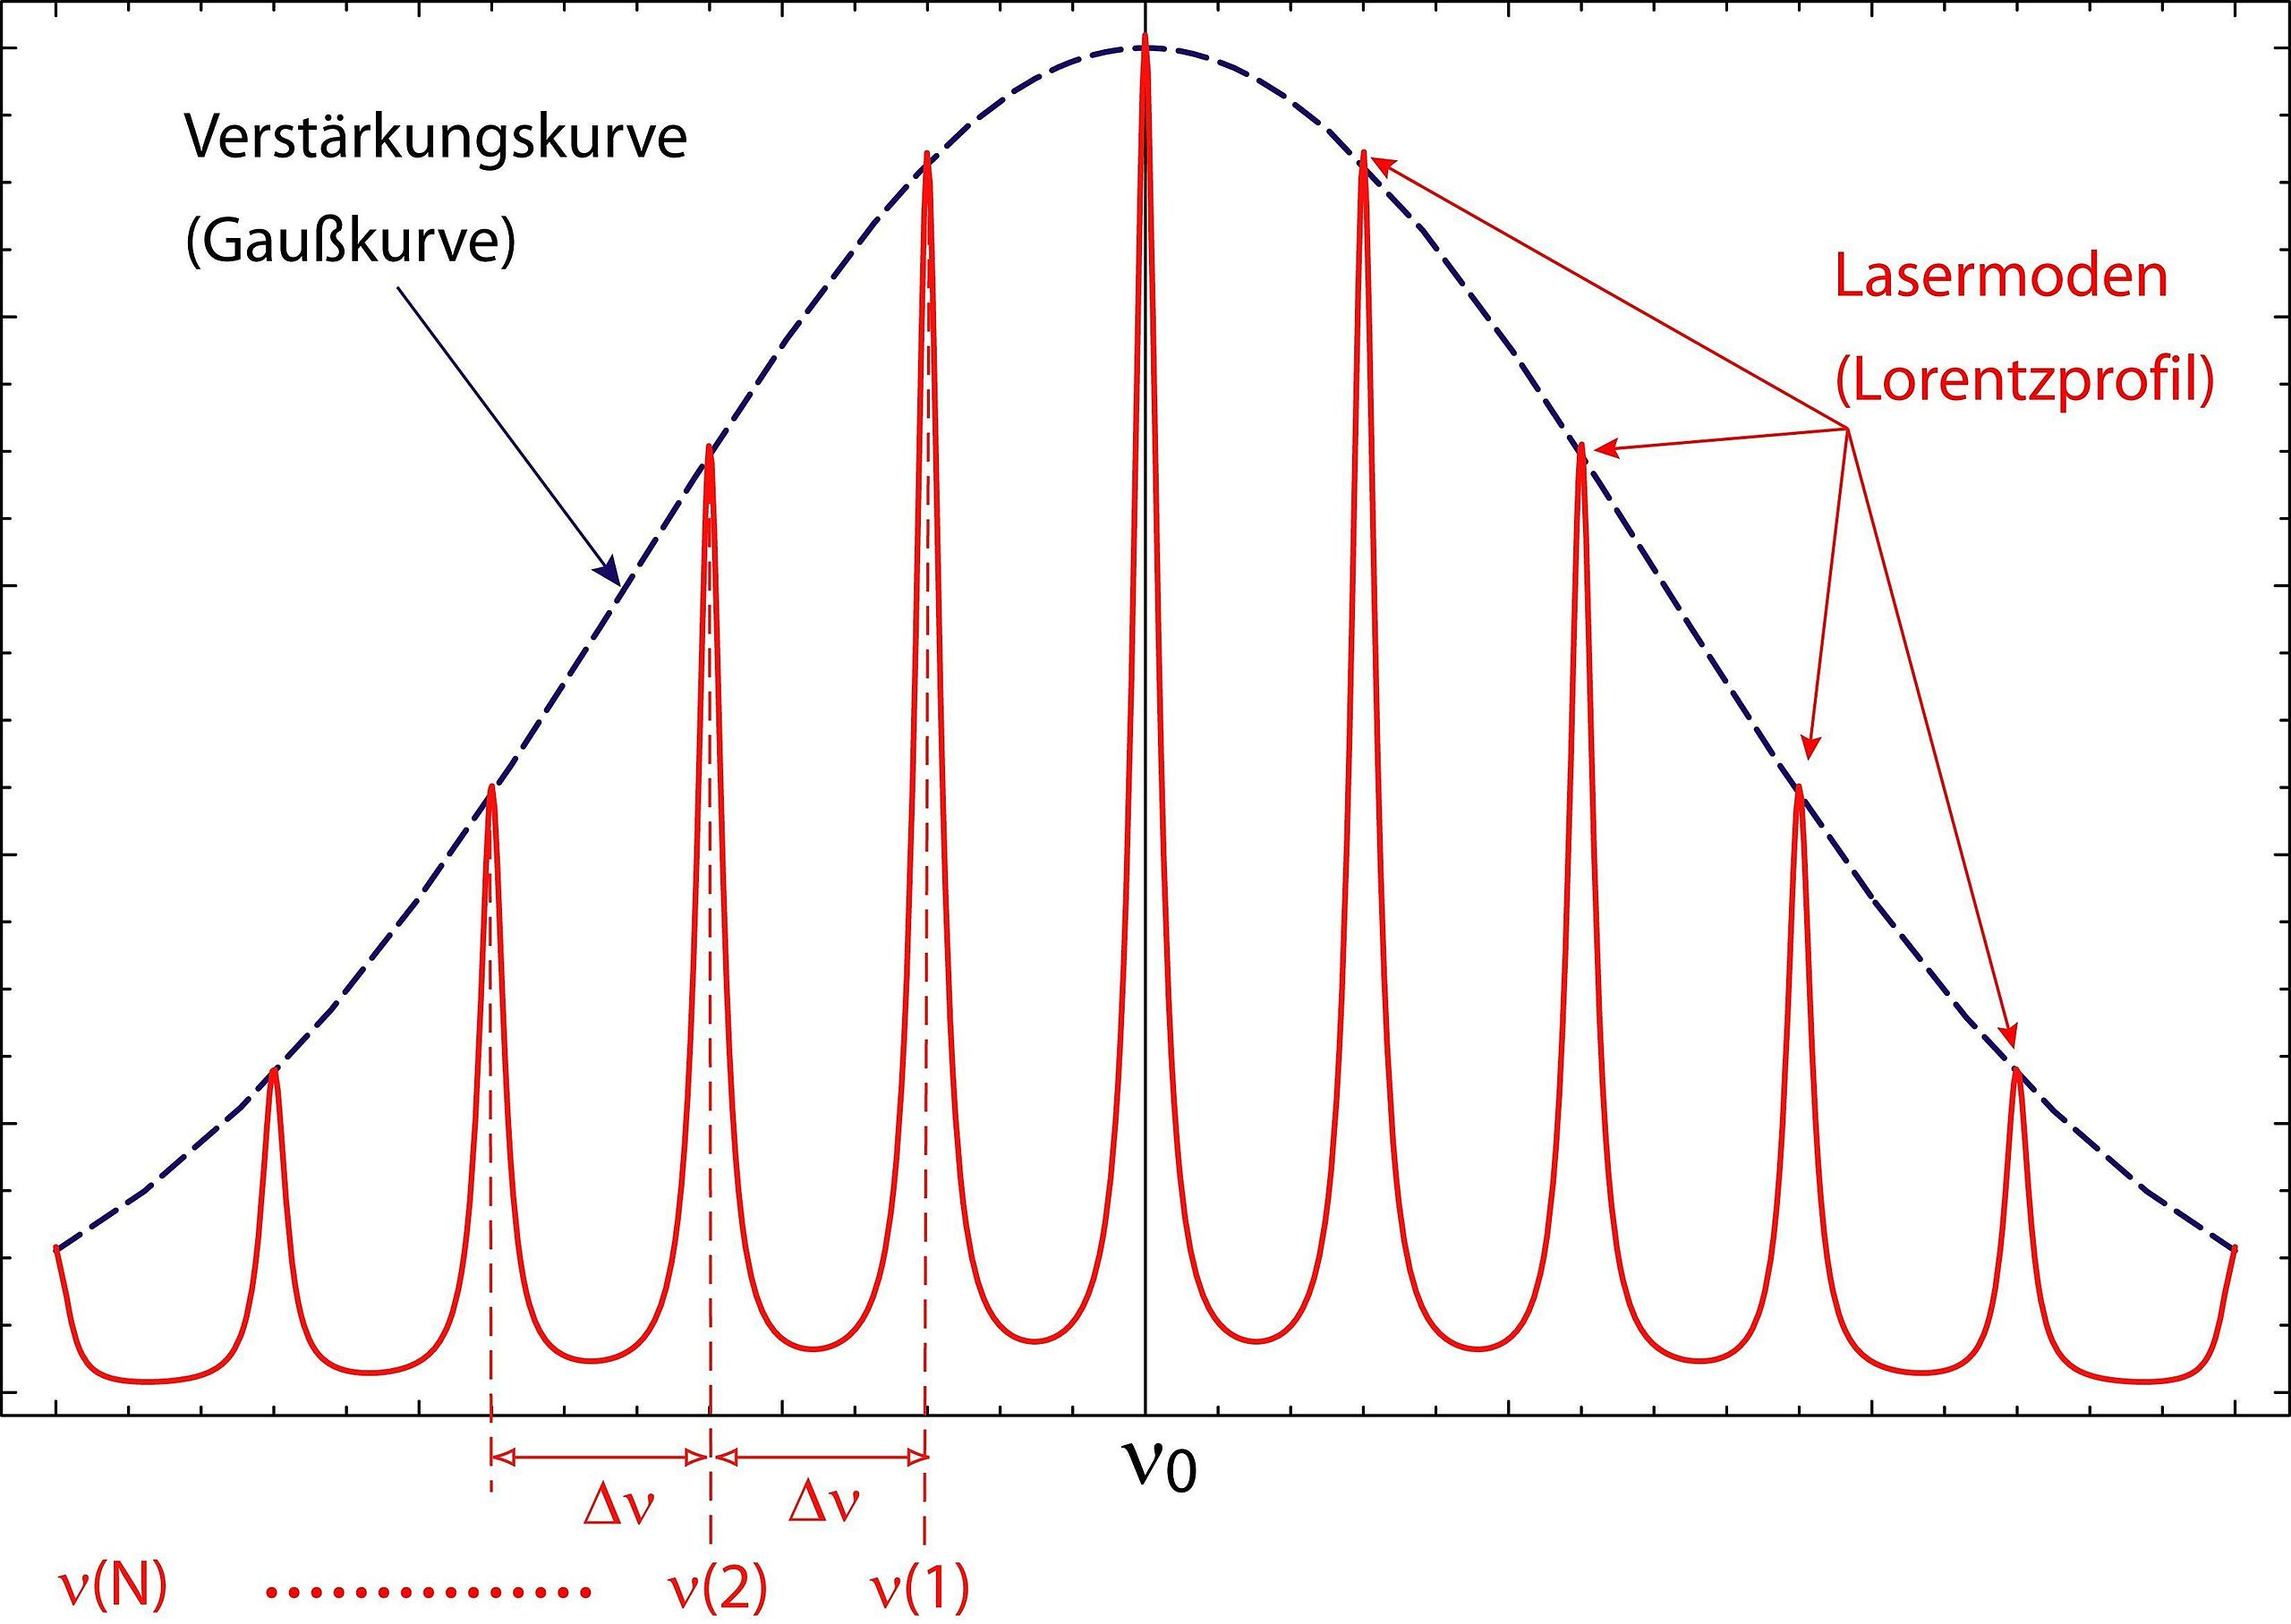
\includegraphics[width=0.6\textwidth]{FzV/LaserModes.jpg}
    \end{figure}
\end{center}
Die Bandbreite ist die Halbwertsbreite der Lasermoden.
Es werden nur solche angeregt, welche innerhalb der Verstärkungskurve (also dem Resonanzbereich) des Resonators liegen.\\\\
\textbf{single-mode Betrieb eines Lasers:}\\
Wenn man einen Laser mit einer hohen Wellenlängenstabilität benötigt, greift man oft auf einen single-mode Laser zurück.
Diese oszilliere nur auch einer Resonator-Eigenschwingung und geben somit nur eine Mode vonsich.
Praktisch wird dies so umgesetzt, das der Laserstrahl ein sogenanntes Fabry-Perot-Ethalon\footnote{Dünnes, beidseitig verspiegeltes Blättchen. Funktionsweise ähnlich zum Faby-Perot-Interferometer} passiert.
Eine Mode kann dies nur passieren und somit hat man eine sehr hohe Wellenlängenstabilität.
\section{Messung von Mischfrequenzen mittels einer Photodiode}
Im Resonator kann es vorkommen, dass die Frequenzen sich leicht unterscheiden.
Somit kommt es zu einer Mischfrequenz, einer Schwebung.
Diese Frequenzen kann man im Detektor nicht mehr detektieren, weswegen man aus der Schwebungsdifferenzfrequenz den Abstand der Moden bestimmt.
\section{Dielektrische Spiegel}
Der Dielektrische Spiegel, oder auch Bragg-Spiegel genannt, ist ein effizienter Reflektor und wird oft in optischen Resonatoren eingesetzt.
Diese besteht aus alternierenden, dünnen Schichten Dielektrika mit unterschiedlichen Brechungindizes.
An jeder dieser vielen Grenzschichten zwischen den einzelnen Lagen, wird ein Teil des Lichtes gemäß den Fesnelschen' Formeln reflektiert.
Ist die Wellenlänge des einfallenden Lichts ein Vielfaches der optischen Weglänge, so interferrieren die Wellen konstruktiv und es entsteht ein relativ guter Reflektor.
\section{3- und 4-Niveaulaser, Termschema für He-Ne-Laser}
\textbf{3- und 4-Niveaulaser}\\
Bei einem Drei-Niveaulaser sind 3 Energieniveaus an der Laseremission beteiligt.
Aus dem Grundzustand werden die Atome durch eine Pumpe in den hohen Zustand 2 (oberes Pumpenniveau) angeregt.
Von dort fällt es in das obere Laserniveau durch spontane Emission.
Um in den Grundzustand wieder zurückzukommen, nutzt man induzierte Emission.
Ein Beispiel für einen 3-Niveaulaser ist der Rubinlaser.
Ein Drei-Niveaulaser hat einen sehr schmale, aber intensive Laserlinie.\\
Bei einem Vier-Niveaulaser sind 4 Energieniveaus an der Laseremission beteiligt.
Hier ist der Unterschied, dass das Atom nicht wie beim Drei-Niveaulaser nach der induzierten Emission in das Grundniveau zurück fällt, sondern in einen weitern Zustand, den unteren Laserniveau.
Von dort fällt es durch spontane Emission in das Grundniveau zurück.
Ein Vorteil hierbei ist, dass die Besetzungsinversionen dauerhaft aufrechterhalten und die Pumpleistung verringer werden kann.
Damit ist ein Dauerstrichlaser realisierbar und nicht wie beim Drei-Niveaulaser ein Pulslaser.
\textbf{Termschema für He-Ne-Laser}\\
Das Termschema eine He-Ne-Lasers sieht wie folgt aus:
\begin{center}
    \begin{figure}[h]
        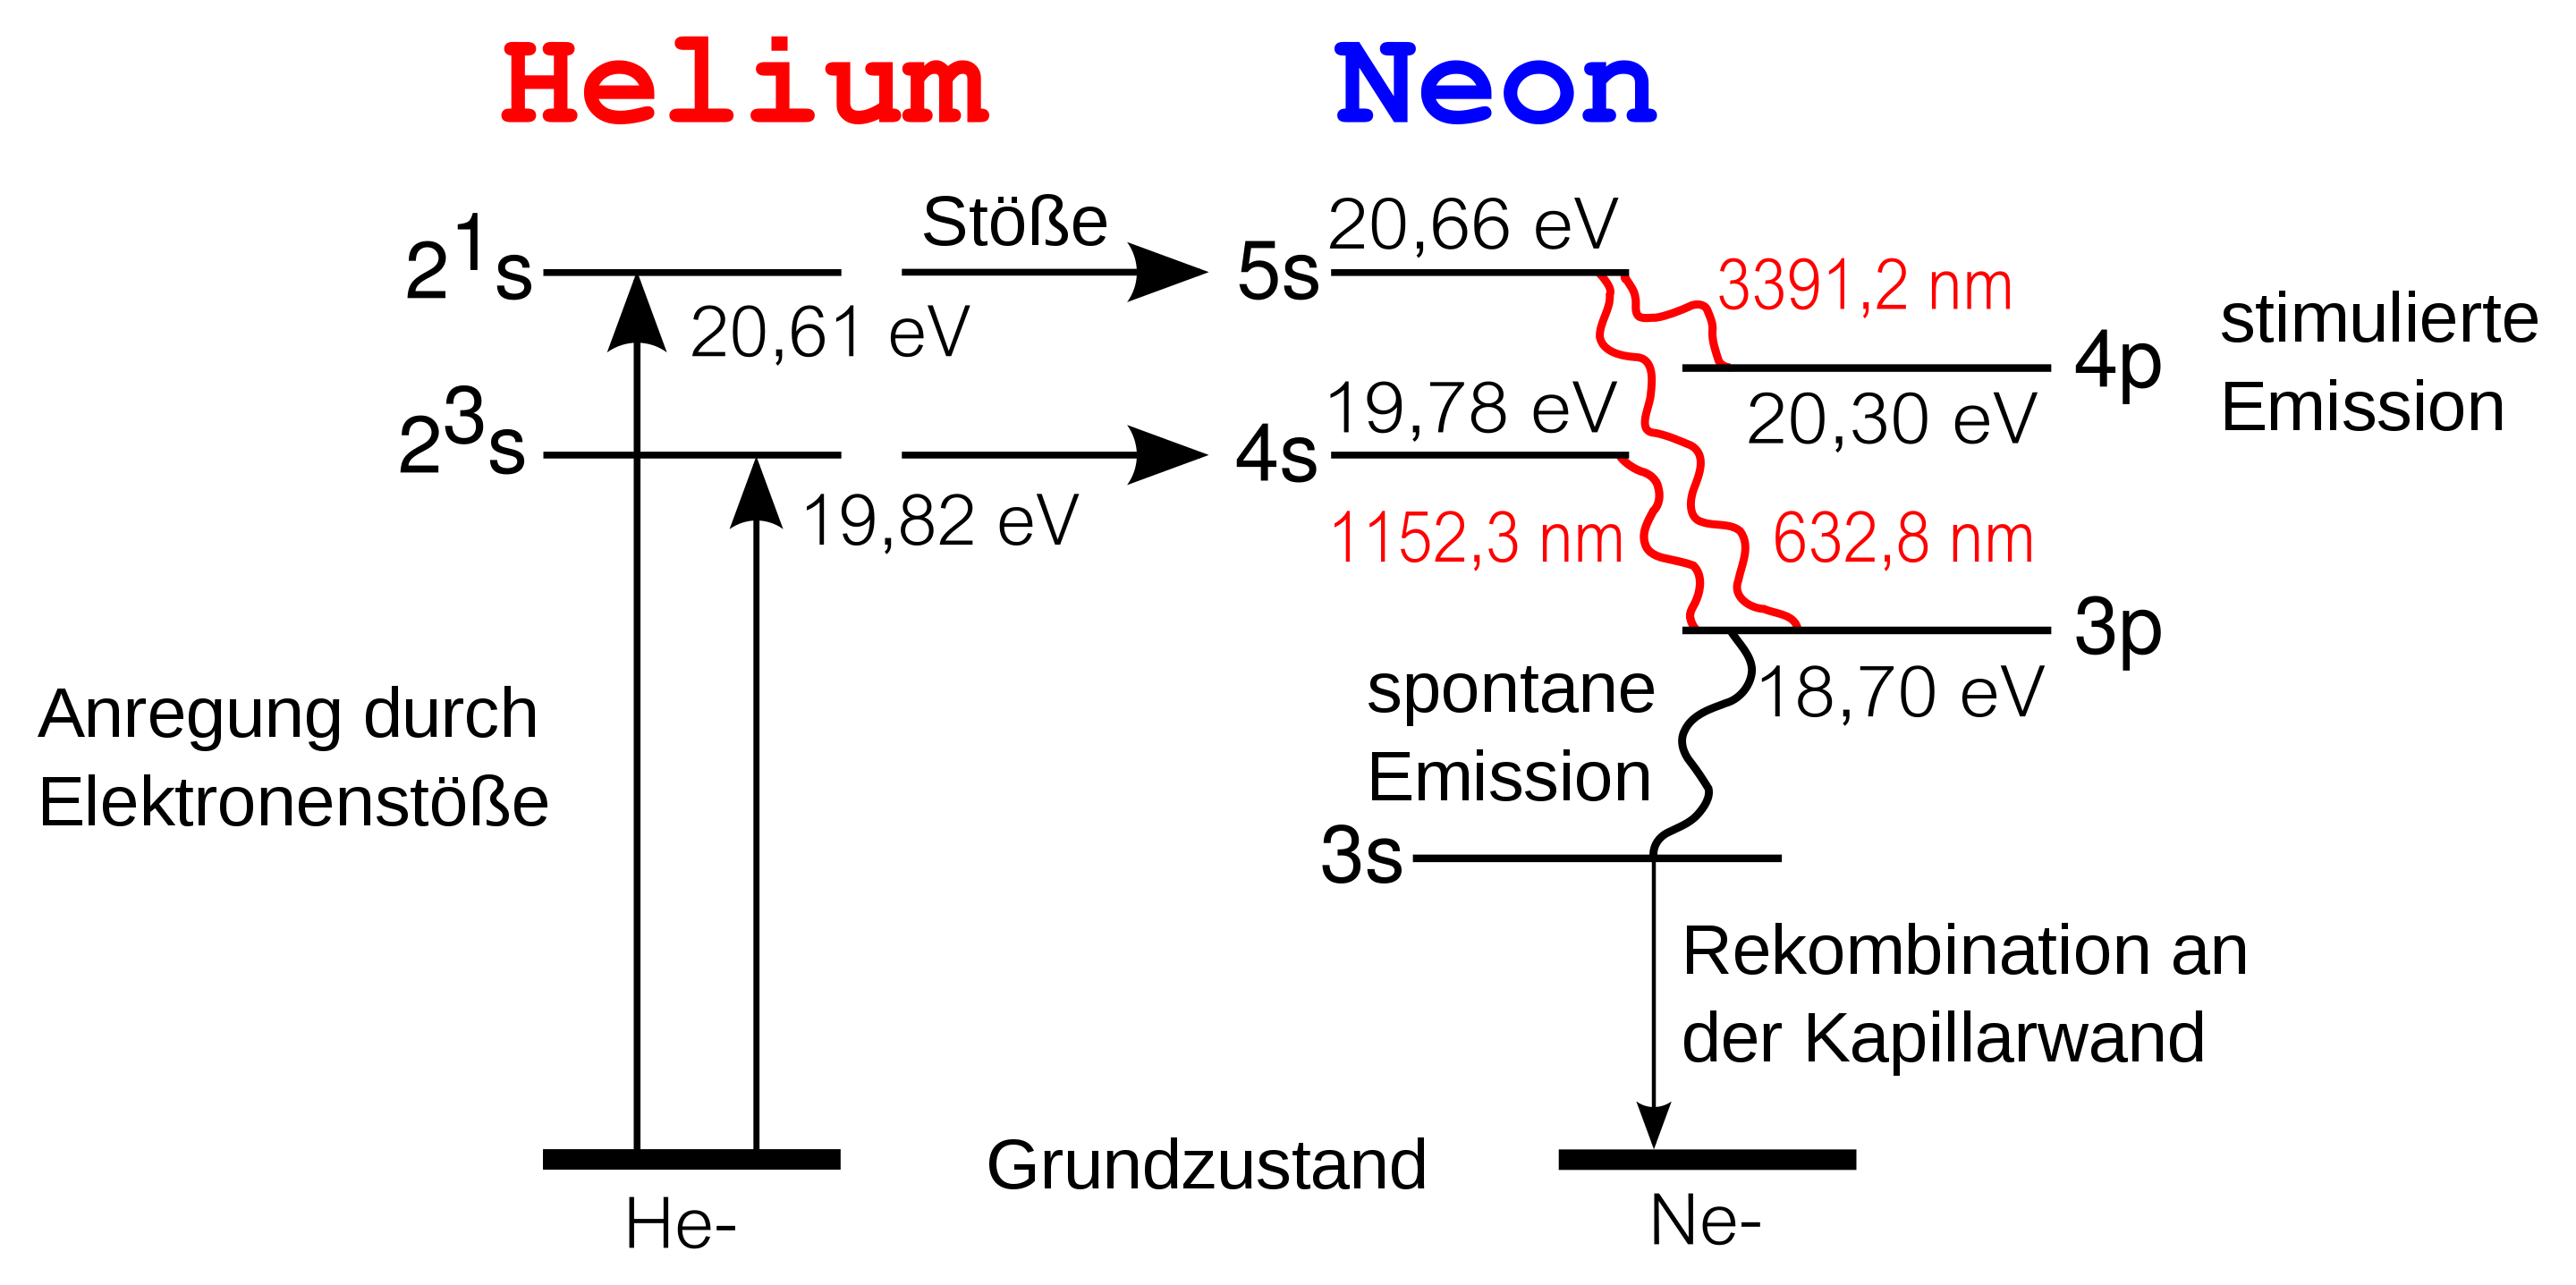
\includegraphics[width=0.6\textwidth]{FzV/TermschemaHeNe.png}
    \end{figure}
\end{center}

\section{Konfokales Fabry-Perot-Interferometer}
Das Fabry-Perot-Interferometer besteht aus zwei teilweise-durchlässigen Spiegel mit ein sehr hohen Reflexionsgrad.
Da durch Variieren des Abstands zwischen den beiden Spiegel sich der optische Weg verändert, kann es bei der Reflexion zu konstruktiver oder destruktiver Interferrenz kommen.
Dies sieht man dann an der Wand durch ein Ringmuster.
\section{Definition der Basiseinheit Meter}
Der Meter wurde definiert als diejenige Strecke, die das Licht im Vakuum innerhalb des Zeitintervalls von 1/299 792 458 Sekunden durchläuft.
\section{Gauß'sche Strahlen, Strahlausbreitung in Medien, Strahlausbreitungsfaktor M$^2$}
\textbf{Gauß'sche Strahlen}\\
Gauß'sche Strahlen sind ein Konzept der Wellenausbreitung in der paraxialen Optik.
Der Querschnitt des Strahles zeigt eine Gauskurve, mit einer in Ausbreitungsrichtung variierenden Breite.
\textbf{Strahlausbreitung in Medien}\\
Strahlen breiten sich in Medien so aus geradlinig aus, damit ihre Laufzeit extremal ist.
\textbf{Strahlausbreitungsfaktor M$^2$}\\
Die Strahlqualität eines Lasers wird durch den M2 Faktor charakteriesiert.
Dieser vergleicht die Form des Laserstrahles mit einem idealen Gauß-Strahls.
\section{Holographie}
Die Holographie beschreit die Aufnahme und Rekonstruktion eines Wellenfeldes, welches von einem beliebigen Objekt ausgeht.



%Versuchsdurchführung
\chapter{Versuchsdurchführung}
Der Versuch wurde bereits vom Betreuer, nach der Anleitung im Skript, aufgebaut.\\
Der Versuchstisch sah wie folgt aus: \\
\begin{figure}[h]
        \centering
        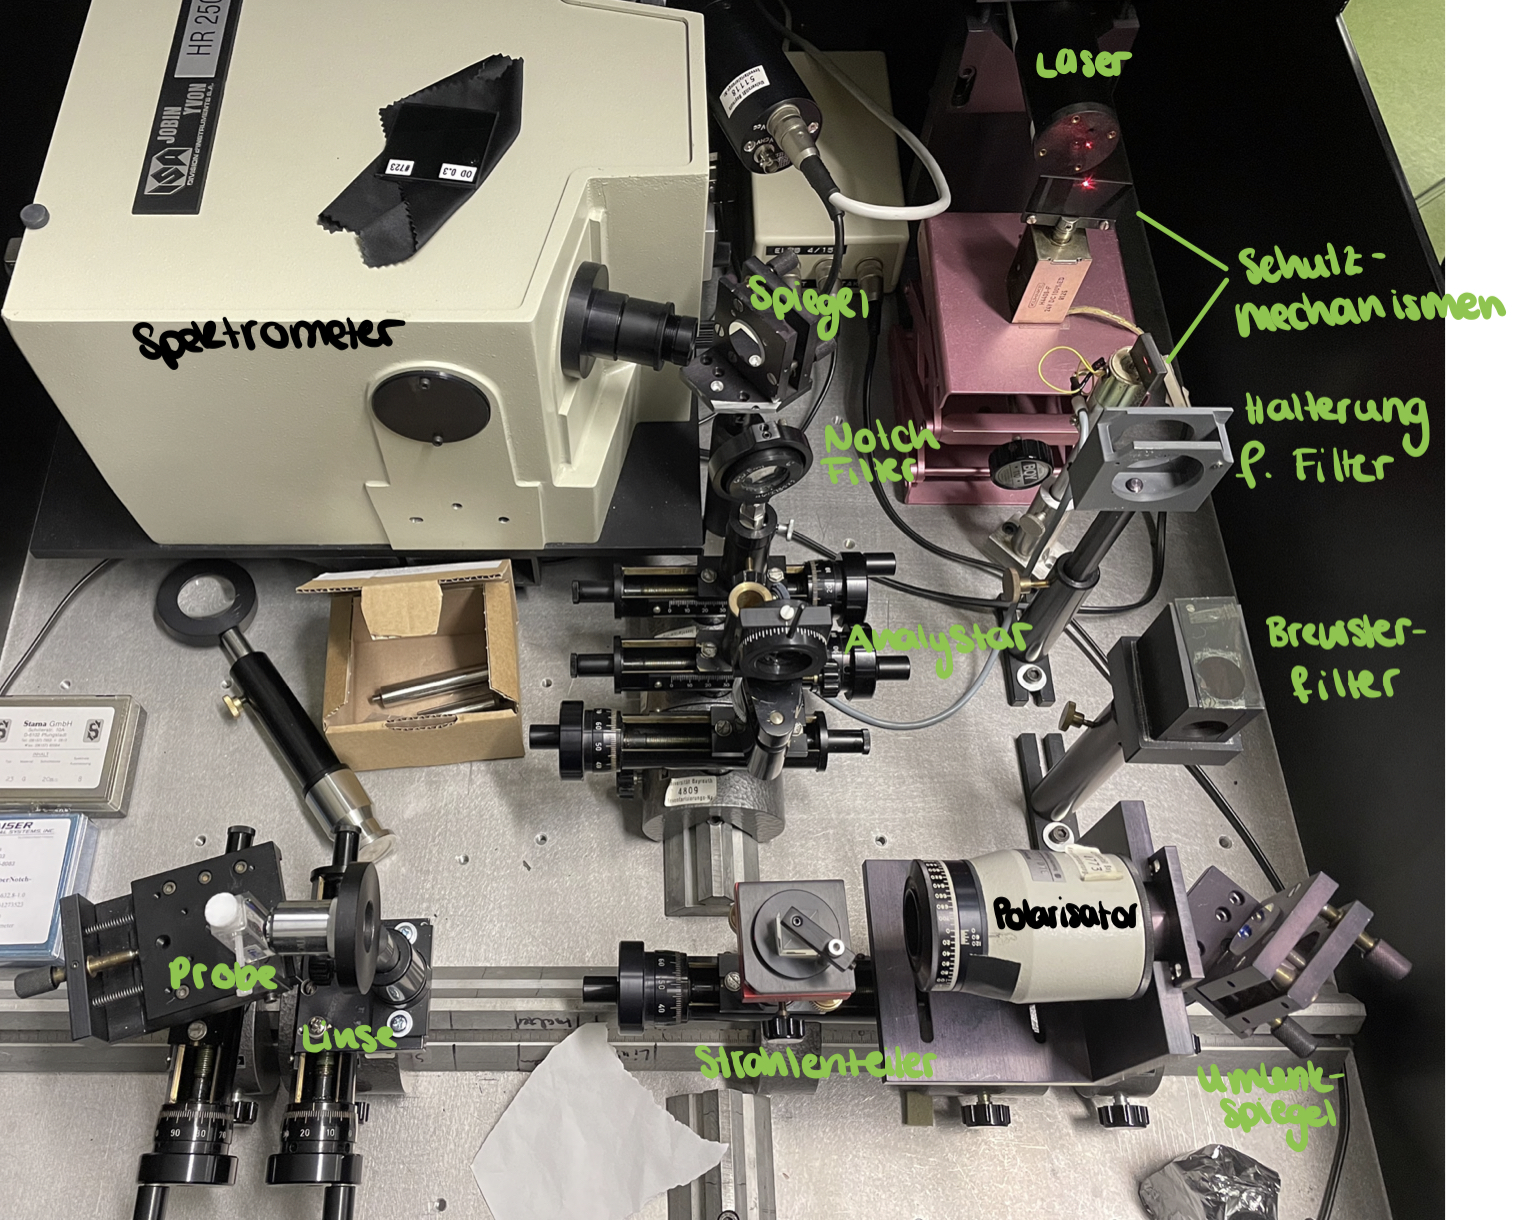
\includegraphics[scale=0.25]{Bilder/Aufbau.jpg}
        \caption{Versuchsaufbau}
\end{figure}\\
Die entsprechend verwendeten Geräte wurden gekennzeichnet. Im Versuch wurde ein 
Helium-Neon Laser verwendet. \\
Die einzigen Veränderungen die während dem Versuch am Aufbau vorgenommen wurden,
war zum einen die Änderung der 
Polarisierung, diese
variierte jedoch nur zwischen 0° bzw. 90° und zum anderen der Wechsel der Proben.\\
Die erste Probe war $CDCl_3$, diese wurde, wie auch die folgenden drei, zuerst in den
Probenhalter eingesetzt und anschließend mit einer Plastik-Schraube fixiert. 
Danach wurde der Probenbehälter an die Linse herangefahren, dies geschah sehr langsam
und vorsichtig.\\
Die Reihenfolge und die Messbereiche, sowie die gemessenen Peaks 
sind dem, im Anhang befindlichen, Protokoll 
zu entnehmen.
\newpage
Während dem Versuch wurden die gerade angesprochenen Peaks der Raman-Linien bestimmt. 
Die folgende Graphik soll veranschaulichen, wie diese bestimmt wurden.\\
\begin{figure}[h]
    \centering
    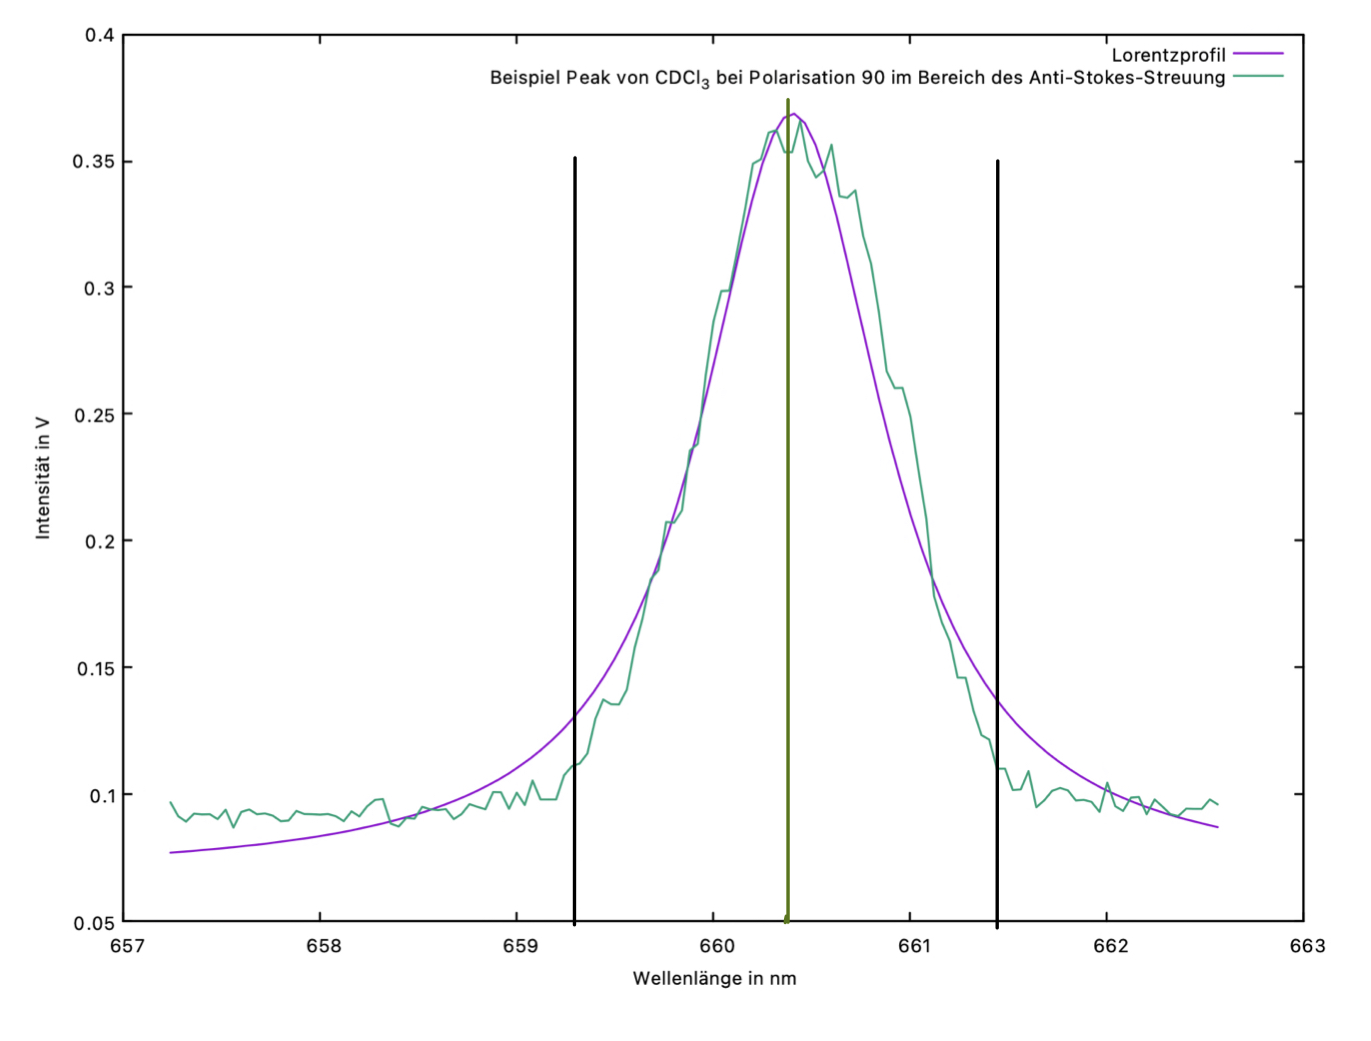
\includegraphics[scale=0.3]{Bilder/Verbesserung_Versuch/plot2.jpg}
    \caption{Skizze der Intensitätsbestimmung der Peaks während dem Versuch, am Beispiel von einem Peak von $CDCl_3$ bei einer Polarisation von 90° im Anti-Stokes-Bereich mit 
    eingezeichneten Lorentzprofil des entsprechenden Peaks.}
    \label{fig:Versuch}
\end{figure}\\
Während der Messung wurde die Breite des Peaks bestimmt, in der Abbildung \ref{fig:Versuch} als schwarze Linien gekennzeichnet, und 
anschließend die ungefähre Mitte geschätzt, dies ist in der Abbildung mithilfe der grünen Linien veranschaulicht wurden. 
In der Mitte wurde die 
Peak-Intensität, mithilfe des Cursors herausgelesen, hierbei wurde darauf geachtet, dass es sich nicht 
um ein Minium bzw. Maximum des 'Rausches' handelte, sondern um einen ungefähren Peak 
des im Kopf abgeschätzten Lorentzprofils. In Abbildung \ref{fig:Versuch} wurde zur Veranschaulichung das Lorentzprofil (lila) des Beispiel-Peaks eingezeichnet. 
Diese wurde jedoch nicht bei jedem Peak berücksichtigt, sondern wie gerade schon erwähnt im Kopf abgeschätzt.\\
Das hat natürlich zur Folge, dass die Intensitätsbestimmung der Peaks einen hohen Fehler haben.

  

%Auswertung
\chapter{Auswertung}
\section{Na-D Linie}
\subsection{Korrekturfaktor des Motors M2}
Die Schwebungsfrequenz der beiden Natrium-D Linien lässt sich wie folgt berechnen:
\begin{equation}
    f_{sch.}=\left|f_{D2}-f_{D1}\right|
\end{equation}
Die Frequenzen der beiden Linien ($f_{D2}$ und $f_{D1}$) lassen sich mithilfe den Literaturwerten für die beiden Wellenlängen der Linien berechnen.\\
Für die erste Natrium-D Linie folgt: $\lambda_{D1}=589,593\,\text{nm}$\\
Und für die zweite D-Linie folgt: $\lambda_{D2}=588,996\,\text{nm}$\\
Diese müssen noch in Frequenzen umgerechnet werden:
\begin{equation}
    f=\frac{c}{\lambda}
\end{equation}
Somit folgt für die Frequenzen der Natrium-D Linien:
\begin{align}
    f_{D1}&=5,083\cdot10^{14}\,\text{Hz}\\
    f_{D2}&=5,090\cdot10^{14}\,\text{Hz}
\end{align}
Und die Schwebungsfrequenz:
\begin{equation}
    f_{sch.}=5,154\cdot10^{11}\,\text{Hz}
\end{equation}
Für die theoretische Schwebungswellenlänge folgt:
\begin{equation}
    \lambda_{{sch.}_{theo.}}=\frac{c}{f_{sch.}}=0,5817\,\text{mm}
\end{equation}\newpage
Um den Korrekturfaktor des Motors $M2$ zu bestimmen, werden die Peaks der Einhüllende bestimmt:
\begin{figure}[h]
    \centering\scalebox{0.8}{% GNUPLOT: LaTeX picture with Postscript
\begingroup
  % Encoding inside the plot.  In the header of your document, this encoding
  % should to defined, e.g., by using
  % \usepackage[cp1252,<other encodings>]{inputenc}
  \inputencoding{cp1252}%
  \makeatletter
  \providecommand\color[2][]{%
    \GenericError{(gnuplot) \space\space\space\@spaces}{%
      Package color not loaded in conjunction with
      terminal option `colourtext'%
    }{See the gnuplot documentation for explanation.%
    }{Either use 'blacktext' in gnuplot or load the package
      color.sty in LaTeX.}%
    \renewcommand\color[2][]{}%
  }%
  \providecommand\includegraphics[2][]{%
    \GenericError{(gnuplot) \space\space\space\@spaces}{%
      Package graphicx or graphics not loaded%
    }{See the gnuplot documentation for explanation.%
    }{The gnuplot epslatex terminal needs graphicx.sty or graphics.sty.}%
    \renewcommand\includegraphics[2][]{}%
  }%
  \providecommand\rotatebox[2]{#2}%
  \@ifundefined{ifGPcolor}{%
    \newif\ifGPcolor
    \GPcolorfalse
  }{}%
  \@ifundefined{ifGPblacktext}{%
    \newif\ifGPblacktext
    \GPblacktexttrue
  }{}%
  % define a \g@addto@macro without @ in the name:
  \let\gplgaddtomacro\g@addto@macro
  % define empty templates for all commands taking text:
  \gdef\gplbacktext{}%
  \gdef\gplfronttext{}%
  \makeatother
  \ifGPblacktext
    % no textcolor at all
    \def\colorrgb#1{}%
    \def\colorgray#1{}%
  \else
    % gray or color?
    \ifGPcolor
      \def\colorrgb#1{\color[rgb]{#1}}%
      \def\colorgray#1{\color[gray]{#1}}%
      \expandafter\def\csname LTw\endcsname{\color{white}}%
      \expandafter\def\csname LTb\endcsname{\color{black}}%
      \expandafter\def\csname LTa\endcsname{\color{black}}%
      \expandafter\def\csname LT0\endcsname{\color[rgb]{1,0,0}}%
      \expandafter\def\csname LT1\endcsname{\color[rgb]{0,1,0}}%
      \expandafter\def\csname LT2\endcsname{\color[rgb]{0,0,1}}%
      \expandafter\def\csname LT3\endcsname{\color[rgb]{1,0,1}}%
      \expandafter\def\csname LT4\endcsname{\color[rgb]{0,1,1}}%
      \expandafter\def\csname LT5\endcsname{\color[rgb]{1,1,0}}%
      \expandafter\def\csname LT6\endcsname{\color[rgb]{0,0,0}}%
      \expandafter\def\csname LT7\endcsname{\color[rgb]{1,0.3,0}}%
      \expandafter\def\csname LT8\endcsname{\color[rgb]{0.5,0.5,0.5}}%
    \else
      % gray
      \def\colorrgb#1{\color{black}}%
      \def\colorgray#1{\color[gray]{#1}}%
      \expandafter\def\csname LTw\endcsname{\color{white}}%
      \expandafter\def\csname LTb\endcsname{\color{black}}%
      \expandafter\def\csname LTa\endcsname{\color{black}}%
      \expandafter\def\csname LT0\endcsname{\color{black}}%
      \expandafter\def\csname LT1\endcsname{\color{black}}%
      \expandafter\def\csname LT2\endcsname{\color{black}}%
      \expandafter\def\csname LT3\endcsname{\color{black}}%
      \expandafter\def\csname LT4\endcsname{\color{black}}%
      \expandafter\def\csname LT5\endcsname{\color{black}}%
      \expandafter\def\csname LT6\endcsname{\color{black}}%
      \expandafter\def\csname LT7\endcsname{\color{black}}%
      \expandafter\def\csname LT8\endcsname{\color{black}}%
    \fi
  \fi
    \setlength{\unitlength}{0.0500bp}%
    \ifx\gptboxheight\undefined%
      \newlength{\gptboxheight}%
      \newlength{\gptboxwidth}%
      \newsavebox{\gptboxtext}%
    \fi%
    \setlength{\fboxrule}{0.5pt}%
    \setlength{\fboxsep}{1pt}%
\begin{picture}(7200.00,5040.00)%
    \gplgaddtomacro\gplbacktext{%
      \csname LTb\endcsname%%
      \put(946,704){\makebox(0,0)[r]{\strut{}$0.02$}}%
      \put(946,1116){\makebox(0,0)[r]{\strut{}$0.03$}}%
      \put(946,1527){\makebox(0,0)[r]{\strut{}$0.04$}}%
      \put(946,1939){\makebox(0,0)[r]{\strut{}$0.05$}}%
      \put(946,2350){\makebox(0,0)[r]{\strut{}$0.06$}}%
      \put(946,2761){\makebox(0,0)[r]{\strut{}$0.07$}}%
      \put(946,3173){\makebox(0,0)[r]{\strut{}$0.08$}}%
      \put(946,3585){\makebox(0,0)[r]{\strut{}$0.09$}}%
      \put(946,3996){\makebox(0,0)[r]{\strut{}$0.1$}}%
      \put(946,4408){\makebox(0,0)[r]{\strut{}$0.11$}}%
      \put(946,4819){\makebox(0,0)[r]{\strut{}$0.12$}}%
      \put(1078,484){\makebox(0,0){\strut{}$30$}}%
      \put(1588,484){\makebox(0,0){\strut{}$32$}}%
      \put(2099,484){\makebox(0,0){\strut{}$34$}}%
      \put(2609,484){\makebox(0,0){\strut{}$36$}}%
      \put(3120,484){\makebox(0,0){\strut{}$38$}}%
      \put(3630,484){\makebox(0,0){\strut{}$40$}}%
      \put(4141,484){\makebox(0,0){\strut{}$42$}}%
      \put(4651,484){\makebox(0,0){\strut{}$44$}}%
      \put(5162,484){\makebox(0,0){\strut{}$46$}}%
      \put(5672,484){\makebox(0,0){\strut{}$48$}}%
      \put(6183,484){\makebox(0,0){\strut{}$50$}}%
      \put(6693,484){\makebox(0,0){\strut{}$52$}}%
    }%
    \gplgaddtomacro\gplfronttext{%
      \csname LTb\endcsname%%
      \put(209,2761){\rotatebox{-270}{\makebox(0,0){\strut{}Intensit\"at [V]}}}%
      \csname LTb\endcsname%%
      \put(6748,2761){\rotatebox{-270}{\makebox(0,0){\strut{}}}}%
      \csname LTb\endcsname%%
      \put(3885,154){\makebox(0,0){\strut{}Motorposition [mm]}}%
      \csname LTb\endcsname%%
      \put(3885,4819){\makebox(0,0){\strut{}}}%
      \csname LTb\endcsname%%
      \put(132,-110){\makebox(0,0)[l]{\strut{}}}%
      \csname LTb\endcsname%%
      \put(5706,4646){\makebox(0,0)[r]{\strut{}Einh\"ullende}}%
      \csname LTb\endcsname%%
      \put(5706,4426){\makebox(0,0)[r]{\strut{}Peaks}}%
    }%
    \gplbacktext
    \put(0,0){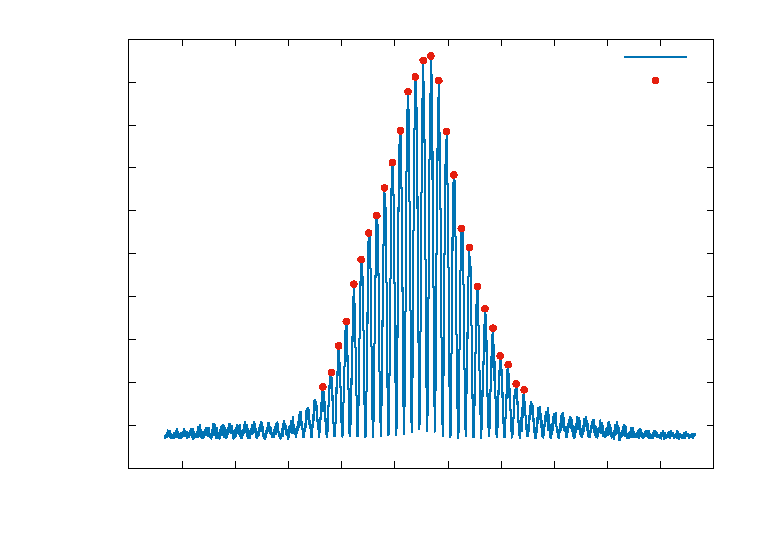
\includegraphics[width={360.00bp},height={252.00bp}]{Dominik/einhuellende_na}}%
    \gplfronttext
  \end{picture}%
\endgroup
}
    \caption{Einhüllende der Na-D Linie mit den eingezeichneten Peaks.}
\end{figure}\\
Der Abstand zwischen zwei Peaks wurde für alle Werte bestimmt und anschließend gemittelt.
Dann erhalten wir den mittleren Abstand:
\begin{equation}
    \bar{p}=\left(0,2913\pm0,0002\right)\,\text{mm}
\end{equation}
Da das Licht die doppelte Weglänge zurücklegt, folgt für die gemessene Wellenlänge der Schwebung:
\begin{equation}
    \lambda_{{sch.}_{mess}}=\left(0,5826\pm0,0004\right)\,\text{mm}
\end{equation}
Der Korrekturfaktor des Motors $M2$ bestimmt sich nun, indem man das Verhältnis aus gemessener und theoretischer Schwebungswellenlänge berechnet:
\begin{equation}
    \beta=\frac{\lambda_{{sch.}_{theo.}}}{\lambda_{{sch.}_{mess}}}
\end{equation}
Somit folgt für den Korrekturfaktor:
\begin{equation}
    \beta=0,998\pm0,001
\end{equation}
Mit diesem kann man die experimentell gemessenen Wegstrecken in die eigentlich gefahrenen Wegstrecken umrechnen:
\begin{equation}
    \lambda_{{sch.}_{theo.}}=\beta\cdot\lambda_{{sch.}_{mess}}
\end{equation}
\subsection{Wellenlänge, Kohärenzlänge und Linienbreite der Linie}
\subsubsection{Wellenlänge bestimmen}
Um die Wellenlänge der Natriumdampflampe zu bestimmen, werden die Peaks des aufgenommenen Spektrums gezählt ($n_{Na}$).
Diese werden anschließend durch die Anzahl der Peaks im Spektrum des Kalibrationslasers ($n_{Laser}$) geteilt und mit dessen Wellenlänge ($\lambda_{Laser}=632,8\,\text{nm}$) multipliziert.
\begin{equation}
    \lambda_{Na}=\frac{n_{Laser}}{n_{Na}}\lambda_{Laser}
\end{equation}\newpage
Um die Peaks zu zählen, wird ein Peakfinder (Python-Programm) genutzt:
\begin{figure}[h]
    \centering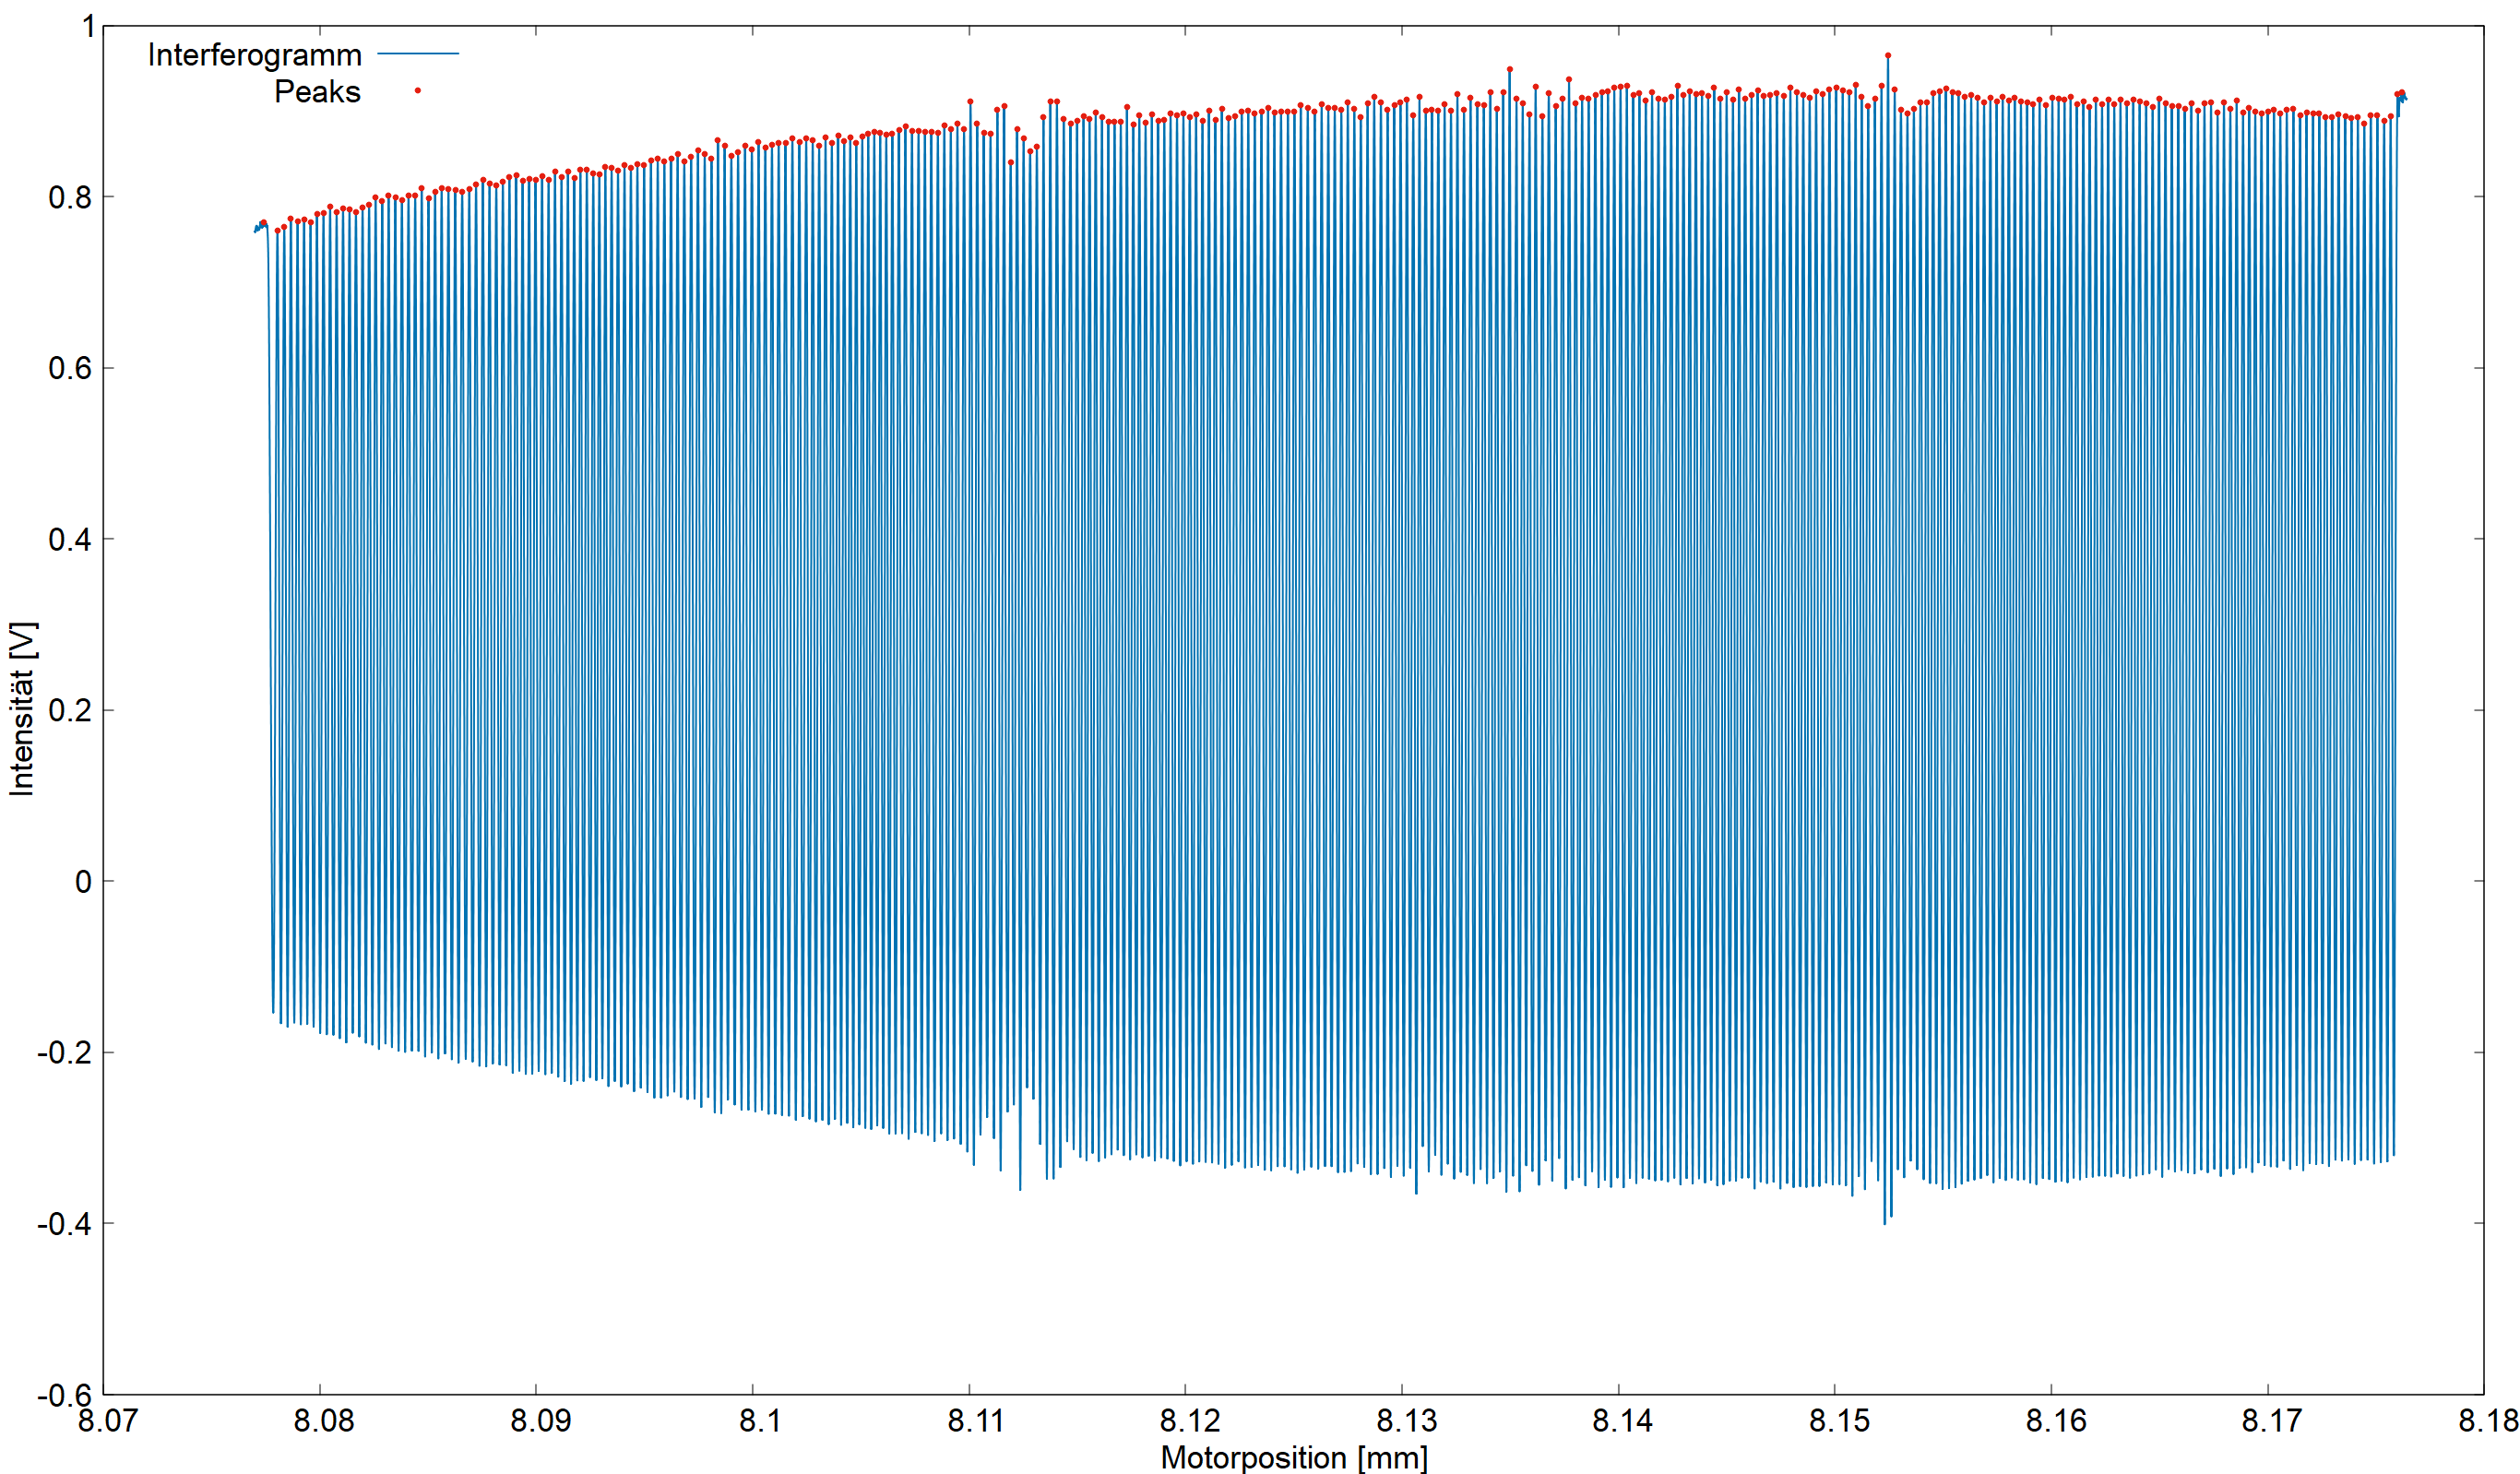
\includegraphics[width=\textwidth]{Dominik/test2.png}
    \caption{Interferogramm der Na-D Linie mit eingezeichneten Peaks.}
\end{figure}\\
Wenn man nun einen Ausschnitt etwas genauer betrachtet:
\begin{figure}[h]
    \centering\subfigure[Na-D Linie]{\scalebox{0.7}{% GNUPLOT: LaTeX picture with Postscript
\begingroup
  % Encoding inside the plot.  In the header of your document, this encoding
  % should to defined, e.g., by using
  % \usepackage[cp1252,<other encodings>]{inputenc}
  \inputencoding{cp1252}%
  \makeatletter
  \providecommand\color[2][]{%
    \GenericError{(gnuplot) \space\space\space\@spaces}{%
      Package color not loaded in conjunction with
      terminal option `colourtext'%
    }{See the gnuplot documentation for explanation.%
    }{Either use 'blacktext' in gnuplot or load the package
      color.sty in LaTeX.}%
    \renewcommand\color[2][]{}%
  }%
  \providecommand\includegraphics[2][]{%
    \GenericError{(gnuplot) \space\space\space\@spaces}{%
      Package graphicx or graphics not loaded%
    }{See the gnuplot documentation for explanation.%
    }{The gnuplot epslatex terminal needs graphicx.sty or graphics.sty.}%
    \renewcommand\includegraphics[2][]{}%
  }%
  \providecommand\rotatebox[2]{#2}%
  \@ifundefined{ifGPcolor}{%
    \newif\ifGPcolor
    \GPcolorfalse
  }{}%
  \@ifundefined{ifGPblacktext}{%
    \newif\ifGPblacktext
    \GPblacktexttrue
  }{}%
  % define a \g@addto@macro without @ in the name:
  \let\gplgaddtomacro\g@addto@macro
  % define empty templates for all commands taking text:
  \gdef\gplbacktext{}%
  \gdef\gplfronttext{}%
  \makeatother
  \ifGPblacktext
    % no textcolor at all
    \def\colorrgb#1{}%
    \def\colorgray#1{}%
  \else
    % gray or color?
    \ifGPcolor
      \def\colorrgb#1{\color[rgb]{#1}}%
      \def\colorgray#1{\color[gray]{#1}}%
      \expandafter\def\csname LTw\endcsname{\color{white}}%
      \expandafter\def\csname LTb\endcsname{\color{black}}%
      \expandafter\def\csname LTa\endcsname{\color{black}}%
      \expandafter\def\csname LT0\endcsname{\color[rgb]{1,0,0}}%
      \expandafter\def\csname LT1\endcsname{\color[rgb]{0,1,0}}%
      \expandafter\def\csname LT2\endcsname{\color[rgb]{0,0,1}}%
      \expandafter\def\csname LT3\endcsname{\color[rgb]{1,0,1}}%
      \expandafter\def\csname LT4\endcsname{\color[rgb]{0,1,1}}%
      \expandafter\def\csname LT5\endcsname{\color[rgb]{1,1,0}}%
      \expandafter\def\csname LT6\endcsname{\color[rgb]{0,0,0}}%
      \expandafter\def\csname LT7\endcsname{\color[rgb]{1,0.3,0}}%
      \expandafter\def\csname LT8\endcsname{\color[rgb]{0.5,0.5,0.5}}%
    \else
      % gray
      \def\colorrgb#1{\color{black}}%
      \def\colorgray#1{\color[gray]{#1}}%
      \expandafter\def\csname LTw\endcsname{\color{white}}%
      \expandafter\def\csname LTb\endcsname{\color{black}}%
      \expandafter\def\csname LTa\endcsname{\color{black}}%
      \expandafter\def\csname LT0\endcsname{\color{black}}%
      \expandafter\def\csname LT1\endcsname{\color{black}}%
      \expandafter\def\csname LT2\endcsname{\color{black}}%
      \expandafter\def\csname LT3\endcsname{\color{black}}%
      \expandafter\def\csname LT4\endcsname{\color{black}}%
      \expandafter\def\csname LT5\endcsname{\color{black}}%
      \expandafter\def\csname LT6\endcsname{\color{black}}%
      \expandafter\def\csname LT7\endcsname{\color{black}}%
      \expandafter\def\csname LT8\endcsname{\color{black}}%
    \fi
  \fi
    \setlength{\unitlength}{0.0500bp}%
    \ifx\gptboxheight\undefined%
      \newlength{\gptboxheight}%
      \newlength{\gptboxwidth}%
      \newsavebox{\gptboxtext}%
    \fi%
    \setlength{\fboxrule}{0.5pt}%
    \setlength{\fboxsep}{1pt}%
\begin{picture}(7200.00,5040.00)%
    \gplgaddtomacro\gplbacktext{%
      \csname LTb\endcsname%%
      \put(946,704){\makebox(0,0)[r]{\strut{}$-0.4$}}%
      \put(946,1253){\makebox(0,0)[r]{\strut{}$-0.2$}}%
      \put(946,1801){\makebox(0,0)[r]{\strut{}$0$}}%
      \put(946,2350){\makebox(0,0)[r]{\strut{}$0.2$}}%
      \put(946,2899){\makebox(0,0)[r]{\strut{}$0.4$}}%
      \put(946,3447){\makebox(0,0)[r]{\strut{}$0.6$}}%
      \put(946,3996){\makebox(0,0)[r]{\strut{}$0.8$}}%
      \put(946,4545){\makebox(0,0)[r]{\strut{}$1$}}%
      \put(1078,484){\makebox(0,0){\strut{}$8.12$}}%
      \put(2201,484){\makebox(0,0){\strut{}$8.122$}}%
      \put(3324,484){\makebox(0,0){\strut{}$8.124$}}%
      \put(4447,484){\makebox(0,0){\strut{}$8.126$}}%
      \put(5570,484){\makebox(0,0){\strut{}$8.128$}}%
      \put(6693,484){\makebox(0,0){\strut{}$8.13$}}%
    }%
    \gplgaddtomacro\gplfronttext{%
      \csname LTb\endcsname%%
      \put(209,2761){\rotatebox{-270}{\makebox(0,0){\strut{}Intensit\"at [V]}}}%
      \csname LTb\endcsname%%
      \put(6748,2761){\rotatebox{-270}{\makebox(0,0){\strut{}}}}%
      \csname LTb\endcsname%%
      \put(3885,154){\makebox(0,0){\strut{}Motorposition [mm]}}%
      \csname LTb\endcsname%%
      \put(3885,4819){\makebox(0,0){\strut{}}}%
      \csname LTb\endcsname%%
      \put(132,-110){\makebox(0,0)[l]{\strut{}}}%
      \csname LTb\endcsname%%
      \put(5706,4646){\makebox(0,0)[r]{\strut{}Interferogramm}}%
      \csname LTb\endcsname%%
      \put(5706,4426){\makebox(0,0)[r]{\strut{}Peaks}}%
    }%
    \gplbacktext
    \put(0,0){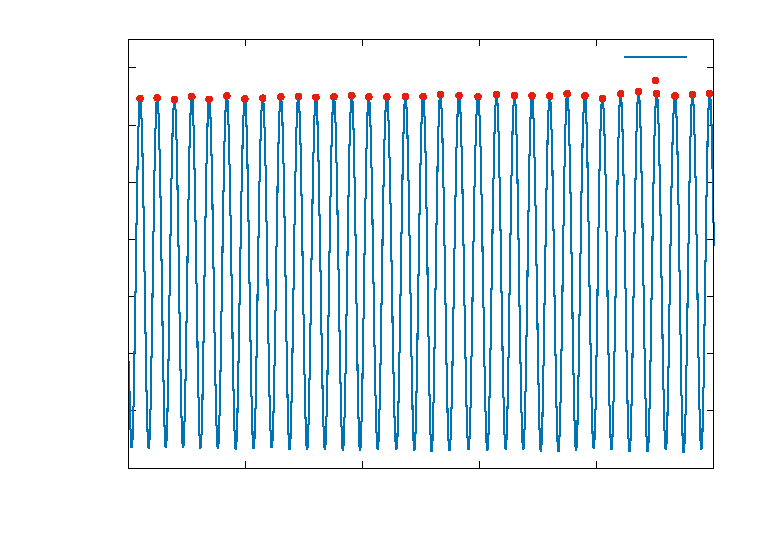
\includegraphics[width={360.00bp},height={252.00bp}]{Dominik/interferogram_na}}%
    \gplfronttext
  \end{picture}%
\endgroup
}}\\
    \subfigure[HeNe-Laser]{\scalebox{0.7}{% GNUPLOT: LaTeX picture with Postscript
\begingroup
  % Encoding inside the plot.  In the header of your document, this encoding
  % should to defined, e.g., by using
  % \usepackage[cp1252,<other encodings>]{inputenc}
  \inputencoding{cp1252}%
  \makeatletter
  \providecommand\color[2][]{%
    \GenericError{(gnuplot) \space\space\space\@spaces}{%
      Package color not loaded in conjunction with
      terminal option `colourtext'%
    }{See the gnuplot documentation for explanation.%
    }{Either use 'blacktext' in gnuplot or load the package
      color.sty in LaTeX.}%
    \renewcommand\color[2][]{}%
  }%
  \providecommand\includegraphics[2][]{%
    \GenericError{(gnuplot) \space\space\space\@spaces}{%
      Package graphicx or graphics not loaded%
    }{See the gnuplot documentation for explanation.%
    }{The gnuplot epslatex terminal needs graphicx.sty or graphics.sty.}%
    \renewcommand\includegraphics[2][]{}%
  }%
  \providecommand\rotatebox[2]{#2}%
  \@ifundefined{ifGPcolor}{%
    \newif\ifGPcolor
    \GPcolorfalse
  }{}%
  \@ifundefined{ifGPblacktext}{%
    \newif\ifGPblacktext
    \GPblacktexttrue
  }{}%
  % define a \g@addto@macro without @ in the name:
  \let\gplgaddtomacro\g@addto@macro
  % define empty templates for all commands taking text:
  \gdef\gplbacktext{}%
  \gdef\gplfronttext{}%
  \makeatother
  \ifGPblacktext
    % no textcolor at all
    \def\colorrgb#1{}%
    \def\colorgray#1{}%
  \else
    % gray or color?
    \ifGPcolor
      \def\colorrgb#1{\color[rgb]{#1}}%
      \def\colorgray#1{\color[gray]{#1}}%
      \expandafter\def\csname LTw\endcsname{\color{white}}%
      \expandafter\def\csname LTb\endcsname{\color{black}}%
      \expandafter\def\csname LTa\endcsname{\color{black}}%
      \expandafter\def\csname LT0\endcsname{\color[rgb]{1,0,0}}%
      \expandafter\def\csname LT1\endcsname{\color[rgb]{0,1,0}}%
      \expandafter\def\csname LT2\endcsname{\color[rgb]{0,0,1}}%
      \expandafter\def\csname LT3\endcsname{\color[rgb]{1,0,1}}%
      \expandafter\def\csname LT4\endcsname{\color[rgb]{0,1,1}}%
      \expandafter\def\csname LT5\endcsname{\color[rgb]{1,1,0}}%
      \expandafter\def\csname LT6\endcsname{\color[rgb]{0,0,0}}%
      \expandafter\def\csname LT7\endcsname{\color[rgb]{1,0.3,0}}%
      \expandafter\def\csname LT8\endcsname{\color[rgb]{0.5,0.5,0.5}}%
    \else
      % gray
      \def\colorrgb#1{\color{black}}%
      \def\colorgray#1{\color[gray]{#1}}%
      \expandafter\def\csname LTw\endcsname{\color{white}}%
      \expandafter\def\csname LTb\endcsname{\color{black}}%
      \expandafter\def\csname LTa\endcsname{\color{black}}%
      \expandafter\def\csname LT0\endcsname{\color{black}}%
      \expandafter\def\csname LT1\endcsname{\color{black}}%
      \expandafter\def\csname LT2\endcsname{\color{black}}%
      \expandafter\def\csname LT3\endcsname{\color{black}}%
      \expandafter\def\csname LT4\endcsname{\color{black}}%
      \expandafter\def\csname LT5\endcsname{\color{black}}%
      \expandafter\def\csname LT6\endcsname{\color{black}}%
      \expandafter\def\csname LT7\endcsname{\color{black}}%
      \expandafter\def\csname LT8\endcsname{\color{black}}%
    \fi
  \fi
    \setlength{\unitlength}{0.0500bp}%
    \ifx\gptboxheight\undefined%
      \newlength{\gptboxheight}%
      \newlength{\gptboxwidth}%
      \newsavebox{\gptboxtext}%
    \fi%
    \setlength{\fboxrule}{0.5pt}%
    \setlength{\fboxsep}{1pt}%
\begin{picture}(7200.00,5040.00)%
    \gplgaddtomacro\gplbacktext{%
      \csname LTb\endcsname%%
      \put(946,704){\makebox(0,0)[r]{\strut{}$-0.1$}}%
      \put(946,1218){\makebox(0,0)[r]{\strut{}$0$}}%
      \put(946,1733){\makebox(0,0)[r]{\strut{}$0.1$}}%
      \put(946,2247){\makebox(0,0)[r]{\strut{}$0.2$}}%
      \put(946,2762){\makebox(0,0)[r]{\strut{}$0.3$}}%
      \put(946,3276){\makebox(0,0)[r]{\strut{}$0.4$}}%
      \put(946,3790){\makebox(0,0)[r]{\strut{}$0.5$}}%
      \put(946,4305){\makebox(0,0)[r]{\strut{}$0.6$}}%
      \put(946,4819){\makebox(0,0)[r]{\strut{}$0.7$}}%
      \put(1078,484){\makebox(0,0){\strut{}$8.12$}}%
      \put(2223,484){\makebox(0,0){\strut{}$8.122$}}%
      \put(3368,484){\makebox(0,0){\strut{}$8.124$}}%
      \put(4513,484){\makebox(0,0){\strut{}$8.126$}}%
      \put(5658,484){\makebox(0,0){\strut{}$8.128$}}%
      \put(6803,484){\makebox(0,0){\strut{}$8.13$}}%
    }%
    \gplgaddtomacro\gplfronttext{%
      \csname LTb\endcsname%%
      \put(209,2761){\rotatebox{-270}{\makebox(0,0){\strut{}Intensit\"at [V]}}}%
      \put(3940,154){\makebox(0,0){\strut{}Motorposition [mm]}}%
      \csname LTb\endcsname%%
      \put(5816,4646){\makebox(0,0)[r]{\strut{}Interferogramm}}%
      \csname LTb\endcsname%%
      \put(5816,4426){\makebox(0,0)[r]{\strut{}Peaks}}%
    }%
    \gplbacktext
    \put(0,0){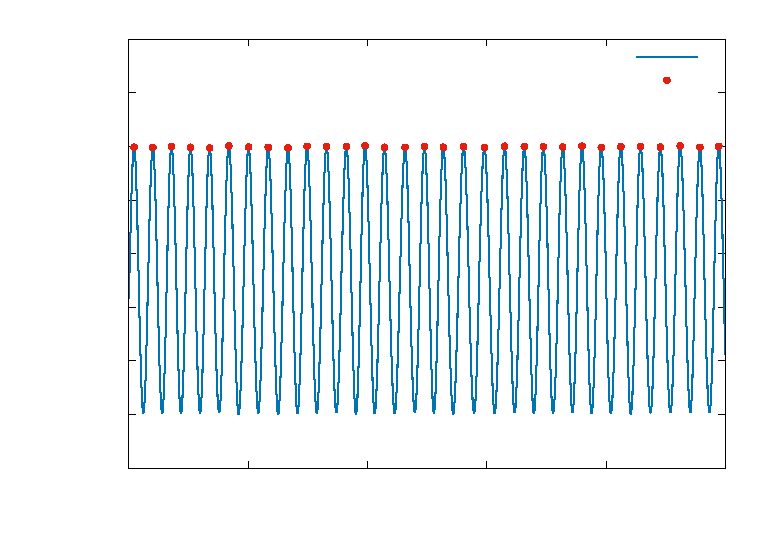
\includegraphics[width={360.00bp},height={252.00bp}]{Dominik/interferogram_nala}}%
    \gplfronttext
  \end{picture}%
\endgroup
}}
    \caption{Ausschnitt aus dem Interferogrammen der Na-D Linie (a) und des HeNe-Lasers (b) mit eingezeichneten Peaks}
\end{figure}\newpage
Wir nehmen an, dass der Peak-finder die Peaks bis zu einen Peak genau findet.
Somit folgt für die Peaks im Spektrum der Natriumdampflampe:
\begin{equation}
    n_{Na}=331\pm1
\end{equation}
Und für den Lasers:
\begin{equation}
    n_{Laser}=307\pm1
\end{equation}
Somit folgt für die Wellenlänge der Natriumdampflampe:
\begin{equation}
    \lambda_{Na}=\left(587\pm3\right)\,\text{nm}
\end{equation}
Der Fehler wurde über eine Fehlerfortpflanzung berechnet:
\begin{align}
    s_{\lambda} &= \sqrt{\left(\frac{\partial \lambda_{Na}}{\partial n_{Laser}}\cdot s_{n_{Laser}}\right)^2+ \left(\frac{\partial \lambda_{Na}}{\partial n_{Na}}\cdot s_{n_{Na}}\right)^2}\\
                &= \sqrt{\left(\frac{\lambda_L}{n_{Na}} \cdot s_{n_{Laser}}\right)^2 + \left(\frac{\lambda_L \cdot n_L}{n^2_{Na}} \cdot s_{n_{Na}}\right)^2 }
\end{align}
Wenn man nun den gemessenen Wert der Natrium-D Linie mit den theoretischen Werten der Natrium-D Linie vergleicht $(\lambda_{D1}=589,593\,\text{nm}; \lambda_{D2}=588,996\,\text{nm})$, sieht man das der gemessene Wert mit seinen Fehler die tatsächlichen Werte einschließt.
%Die so bestimmte Wellenlänge mit ihrem Fehler schließen die theoretischen Werte der Natrium-D Linien ein.

\subsubsection{Kohärenzlänge bestimmen}
Die Kohärenzlänge ist die halbe Intervalllänge der Einhüllenden, bei dieser die maximale Intensität  auf $1/e$ abgefallen ist.
Diese kann man direkt aus der Einhüllenden herauslesen.
Für die maximale Intensität wurde gemessen:
\begin{align}
    I_0&=\left(0,0883\pm0,0001\right)\,\text{V}\\ %y-Achsenabstand: 0,0278
    \frac{I_0}{e}&=\left(32,48\pm0,04\right)\,\text{mV}
\end{align}
Hierbei wurde der y-Achsen Offset der Messkurve berücksichtigt.
Dieser ist die Differenz zwischen dem Nullwert des Plots und des Wertes auf den die Intensität abfällt.
%Der y-Achsen Offset ist der Wert, auf den die Linie abfällt, anstatt das diese auf Null abfällt.\\
Somit folgt für die Kohärenzlänge $L$:
\begin{align}
    L&=\beta\cdot\frac{\Delta s\left(\frac{I_0}{e}\right)}{2}\\
    L&=\left(2,5\pm0,1\right)\,\text{mm}
\end{align}\newpage
Graphisch folgt:
\begin{figure}[h]
    \centering\scalebox{0.8}{% GNUPLOT: LaTeX picture with Postscript
\begingroup
  % Encoding inside the plot.  In the header of your document, this encoding
  % should to defined, e.g., by using
  % \usepackage[cp1252,<other encodings>]{inputenc}
  \inputencoding{cp1252}%
  \makeatletter
  \providecommand\color[2][]{%
    \GenericError{(gnuplot) \space\space\space\@spaces}{%
      Package color not loaded in conjunction with
      terminal option `colourtext'%
    }{See the gnuplot documentation for explanation.%
    }{Either use 'blacktext' in gnuplot or load the package
      color.sty in LaTeX.}%
    \renewcommand\color[2][]{}%
  }%
  \providecommand\includegraphics[2][]{%
    \GenericError{(gnuplot) \space\space\space\@spaces}{%
      Package graphicx or graphics not loaded%
    }{See the gnuplot documentation for explanation.%
    }{The gnuplot epslatex terminal needs graphicx.sty or graphics.sty.}%
    \renewcommand\includegraphics[2][]{}%
  }%
  \providecommand\rotatebox[2]{#2}%
  \@ifundefined{ifGPcolor}{%
    \newif\ifGPcolor
    \GPcolorfalse
  }{}%
  \@ifundefined{ifGPblacktext}{%
    \newif\ifGPblacktext
    \GPblacktexttrue
  }{}%
  % define a \g@addto@macro without @ in the name:
  \let\gplgaddtomacro\g@addto@macro
  % define empty templates for all commands taking text:
  \gdef\gplbacktext{}%
  \gdef\gplfronttext{}%
  \makeatother
  \ifGPblacktext
    % no textcolor at all
    \def\colorrgb#1{}%
    \def\colorgray#1{}%
  \else
    % gray or color?
    \ifGPcolor
      \def\colorrgb#1{\color[rgb]{#1}}%
      \def\colorgray#1{\color[gray]{#1}}%
      \expandafter\def\csname LTw\endcsname{\color{white}}%
      \expandafter\def\csname LTb\endcsname{\color{black}}%
      \expandafter\def\csname LTa\endcsname{\color{black}}%
      \expandafter\def\csname LT0\endcsname{\color[rgb]{1,0,0}}%
      \expandafter\def\csname LT1\endcsname{\color[rgb]{0,1,0}}%
      \expandafter\def\csname LT2\endcsname{\color[rgb]{0,0,1}}%
      \expandafter\def\csname LT3\endcsname{\color[rgb]{1,0,1}}%
      \expandafter\def\csname LT4\endcsname{\color[rgb]{0,1,1}}%
      \expandafter\def\csname LT5\endcsname{\color[rgb]{1,1,0}}%
      \expandafter\def\csname LT6\endcsname{\color[rgb]{0,0,0}}%
      \expandafter\def\csname LT7\endcsname{\color[rgb]{1,0.3,0}}%
      \expandafter\def\csname LT8\endcsname{\color[rgb]{0.5,0.5,0.5}}%
    \else
      % gray
      \def\colorrgb#1{\color{black}}%
      \def\colorgray#1{\color[gray]{#1}}%
      \expandafter\def\csname LTw\endcsname{\color{white}}%
      \expandafter\def\csname LTb\endcsname{\color{black}}%
      \expandafter\def\csname LTa\endcsname{\color{black}}%
      \expandafter\def\csname LT0\endcsname{\color{black}}%
      \expandafter\def\csname LT1\endcsname{\color{black}}%
      \expandafter\def\csname LT2\endcsname{\color{black}}%
      \expandafter\def\csname LT3\endcsname{\color{black}}%
      \expandafter\def\csname LT4\endcsname{\color{black}}%
      \expandafter\def\csname LT5\endcsname{\color{black}}%
      \expandafter\def\csname LT6\endcsname{\color{black}}%
      \expandafter\def\csname LT7\endcsname{\color{black}}%
      \expandafter\def\csname LT8\endcsname{\color{black}}%
    \fi
  \fi
    \setlength{\unitlength}{0.0500bp}%
    \ifx\gptboxheight\undefined%
      \newlength{\gptboxheight}%
      \newlength{\gptboxwidth}%
      \newsavebox{\gptboxtext}%
    \fi%
    \setlength{\fboxrule}{0.5pt}%
    \setlength{\fboxsep}{1pt}%
\begin{picture}(7200.00,5040.00)%
    \gplgaddtomacro\gplbacktext{%
      \csname LTb\endcsname%%
      \put(946,704){\makebox(0,0)[r]{\strut{}$0.02$}}%
      \put(946,1116){\makebox(0,0)[r]{\strut{}$0.03$}}%
      \put(946,1527){\makebox(0,0)[r]{\strut{}$0.04$}}%
      \put(946,1939){\makebox(0,0)[r]{\strut{}$0.05$}}%
      \put(946,2350){\makebox(0,0)[r]{\strut{}$0.06$}}%
      \put(946,2761){\makebox(0,0)[r]{\strut{}$0.07$}}%
      \put(946,3173){\makebox(0,0)[r]{\strut{}$0.08$}}%
      \put(946,3585){\makebox(0,0)[r]{\strut{}$0.09$}}%
      \put(946,3996){\makebox(0,0)[r]{\strut{}$0.1$}}%
      \put(946,4408){\makebox(0,0)[r]{\strut{}$0.11$}}%
      \put(946,4819){\makebox(0,0)[r]{\strut{}$0.12$}}%
      \put(1078,484){\makebox(0,0){\strut{}$30$}}%
      \put(1598,484){\makebox(0,0){\strut{}$32$}}%
      \put(2119,484){\makebox(0,0){\strut{}$34$}}%
      \put(2639,484){\makebox(0,0){\strut{}$36$}}%
      \put(3160,484){\makebox(0,0){\strut{}$38$}}%
      \put(3680,484){\makebox(0,0){\strut{}$40$}}%
      \put(4201,484){\makebox(0,0){\strut{}$42$}}%
      \put(4721,484){\makebox(0,0){\strut{}$44$}}%
      \put(5242,484){\makebox(0,0){\strut{}$46$}}%
      \put(5762,484){\makebox(0,0){\strut{}$48$}}%
      \put(6283,484){\makebox(0,0){\strut{}$50$}}%
      \put(6803,484){\makebox(0,0){\strut{}$52$}}%
    }%
    \gplgaddtomacro\gplfronttext{%
      \csname LTb\endcsname%%
      \put(209,2761){\rotatebox{-270}{\makebox(0,0){\strut{}Intensit\"at [V]}}}%
      \put(3940,154){\makebox(0,0){\strut{}Motorposition [mm]}}%
    }%
    \gplbacktext
    \put(0,0){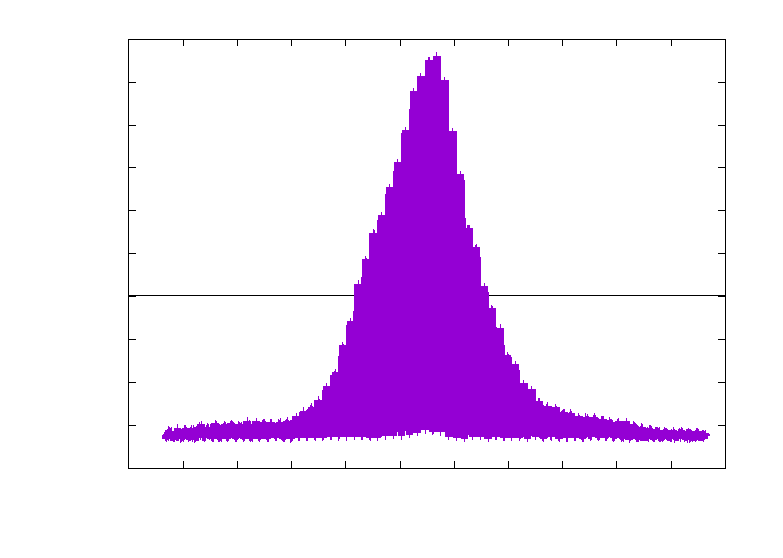
\includegraphics[width={360.00bp},height={252.00bp}]{Dominik/einhuellende_na_I}}%
    \gplfronttext
  \end{picture}%
\endgroup
}
    \caption{Einhüllende des Interferogramms der Na-D Linie mit eingezeichneter $I_0/e$-Intensität}
\end{figure}\\
Da die Einhüllende für die Schnittpunkte mit der $I_0/e$-Gerade per Augenmaß abgelesen wurde, nehmen wir einen Ablesefehler von $0,1\,\text{mm}$ an.
\subsubsection{Linienbreite bestimmen}
Um die Linienbreite zu berechnen muss man erst wissen, um welchen Verbreiterungsmechanismus es sich handelt.
Da die Kurve einer Gauß-Glocke ähnelt, liegt hier eine Dopplerverbreiterung vor (siehe \ref{abbildung_ein}).
Ein Fit dazu findet sich im Kapitel 'Verbreiterungsmechanismus' wieder.
Für diese wurden in den Fragen zur Vorbereitung die Umrechnung zwischen Linienbreite (FWHM-Breite) und Kohärenzlänge (halbe $1/e$-Breite) bestimmt.
Es ist hierbei zu beachten, dass die Linienbreite im k-Raum ausgerechnet wird (Wellenzahlen), um diese nun in den l-Raum umzurechnen folgt:
\begin{align}
    \left|\frac{\Delta k}{\Delta \lambda}\right|&=\left|\frac{dk}{d\lambda}\right|=\frac{2\pi}{\lambda^2}\\
    d\lambda&=dk\cdot\frac{\lambda^2}{2\pi}
\end{align}
Hier steht $dk$ für die FHWM-Breite der Linie im k-Raum, $\lambda$ für gemessene Wellenlänge und $d\lambda$ für die FWHM-Breite im l-Raum.\\
Somit folgt für die Linienbreite einer Dopplerverbreiterten Linie im l-Raum:
\begin{equation}
    \Delta \lambda_{Na}=\left(0,073\pm0,003\right)\,\text{nm}
\end{equation}
Der Fehler wurde über Fehlerfortpflanzung bestimmt:
\begin{align}
    s_{\Delta \lambda_{Na}} &= \sqrt{\left(\frac{\partial \Delta \lambda_{Na}}{\partial L_c} \cdot s_{L_c}\right)^2+\left(\frac{\partial \Delta \lambda_{Na}}{\partial \lambda_{Na}} \cdot s_{\lambda_{Na}}\right)^2} \\
    &= \sqrt{\left(\frac{2 \sqrt{ln(2)} \cdot \lambda^2_{Na}}{L_c^2 \cdot \pi} \cdot s_{L_c}\right)^2+\left(\frac{4 \sqrt{ln(2)}\cdot \lambda_{Na}}{L_c \cdot \pi} \cdot s_{\lambda_{Na}}\right)^2}
\end{align}
\newpage
\subsection{Intensitätsverhältnis und Abstand der beiden Natrium D-Linien}
Bei der Natriumdampflampe liegen die Linien, der D-1 und D-2 Linie sehr nahe zusammen, dies führt zu einer Schwebung.
\begin{figure}[h]
    \centering\scalebox{0.8}{% GNUPLOT: LaTeX picture with Postscript
\begingroup
  % Encoding inside the plot.  In the header of your document, this encoding
  % should to defined, e.g., by using
  % \usepackage[cp1252,<other encodings>]{inputenc}
  \inputencoding{cp1252}%
  \makeatletter
  \providecommand\color[2][]{%
    \GenericError{(gnuplot) \space\space\space\@spaces}{%
      Package color not loaded in conjunction with
      terminal option `colourtext'%
    }{See the gnuplot documentation for explanation.%
    }{Either use 'blacktext' in gnuplot or load the package
      color.sty in LaTeX.}%
    \renewcommand\color[2][]{}%
  }%
  \providecommand\includegraphics[2][]{%
    \GenericError{(gnuplot) \space\space\space\@spaces}{%
      Package graphicx or graphics not loaded%
    }{See the gnuplot documentation for explanation.%
    }{The gnuplot epslatex terminal needs graphicx.sty or graphics.sty.}%
    \renewcommand\includegraphics[2][]{}%
  }%
  \providecommand\rotatebox[2]{#2}%
  \@ifundefined{ifGPcolor}{%
    \newif\ifGPcolor
    \GPcolorfalse
  }{}%
  \@ifundefined{ifGPblacktext}{%
    \newif\ifGPblacktext
    \GPblacktexttrue
  }{}%
  % define a \g@addto@macro without @ in the name:
  \let\gplgaddtomacro\g@addto@macro
  % define empty templates for all commands taking text:
  \gdef\gplbacktext{}%
  \gdef\gplfronttext{}%
  \makeatother
  \ifGPblacktext
    % no textcolor at all
    \def\colorrgb#1{}%
    \def\colorgray#1{}%
  \else
    % gray or color?
    \ifGPcolor
      \def\colorrgb#1{\color[rgb]{#1}}%
      \def\colorgray#1{\color[gray]{#1}}%
      \expandafter\def\csname LTw\endcsname{\color{white}}%
      \expandafter\def\csname LTb\endcsname{\color{black}}%
      \expandafter\def\csname LTa\endcsname{\color{black}}%
      \expandafter\def\csname LT0\endcsname{\color[rgb]{1,0,0}}%
      \expandafter\def\csname LT1\endcsname{\color[rgb]{0,1,0}}%
      \expandafter\def\csname LT2\endcsname{\color[rgb]{0,0,1}}%
      \expandafter\def\csname LT3\endcsname{\color[rgb]{1,0,1}}%
      \expandafter\def\csname LT4\endcsname{\color[rgb]{0,1,1}}%
      \expandafter\def\csname LT5\endcsname{\color[rgb]{1,1,0}}%
      \expandafter\def\csname LT6\endcsname{\color[rgb]{0,0,0}}%
      \expandafter\def\csname LT7\endcsname{\color[rgb]{1,0.3,0}}%
      \expandafter\def\csname LT8\endcsname{\color[rgb]{0.5,0.5,0.5}}%
    \else
      % gray
      \def\colorrgb#1{\color{black}}%
      \def\colorgray#1{\color[gray]{#1}}%
      \expandafter\def\csname LTw\endcsname{\color{white}}%
      \expandafter\def\csname LTb\endcsname{\color{black}}%
      \expandafter\def\csname LTa\endcsname{\color{black}}%
      \expandafter\def\csname LT0\endcsname{\color{black}}%
      \expandafter\def\csname LT1\endcsname{\color{black}}%
      \expandafter\def\csname LT2\endcsname{\color{black}}%
      \expandafter\def\csname LT3\endcsname{\color{black}}%
      \expandafter\def\csname LT4\endcsname{\color{black}}%
      \expandafter\def\csname LT5\endcsname{\color{black}}%
      \expandafter\def\csname LT6\endcsname{\color{black}}%
      \expandafter\def\csname LT7\endcsname{\color{black}}%
      \expandafter\def\csname LT8\endcsname{\color{black}}%
    \fi
  \fi
    \setlength{\unitlength}{0.0500bp}%
    \ifx\gptboxheight\undefined%
      \newlength{\gptboxheight}%
      \newlength{\gptboxwidth}%
      \newsavebox{\gptboxtext}%
    \fi%
    \setlength{\fboxrule}{0.5pt}%
    \setlength{\fboxsep}{1pt}%
\begin{picture}(7200.00,5040.00)%
    \gplgaddtomacro\gplbacktext{%
      \csname LTb\endcsname%%
      \put(946,704){\makebox(0,0)[r]{\strut{}$-0.4$}}%
      \put(946,1292){\makebox(0,0)[r]{\strut{}$-0.2$}}%
      \put(946,1880){\makebox(0,0)[r]{\strut{}$0$}}%
      \put(946,2468){\makebox(0,0)[r]{\strut{}$0.2$}}%
      \put(946,3055){\makebox(0,0)[r]{\strut{}$0.4$}}%
      \put(946,3643){\makebox(0,0)[r]{\strut{}$0.6$}}%
      \put(946,4231){\makebox(0,0)[r]{\strut{}$0.8$}}%
      \put(946,4819){\makebox(0,0)[r]{\strut{}$1$}}%
      \put(1078,484){\makebox(0,0){\strut{}$7.95$}}%
      \put(1794,484){\makebox(0,0){\strut{}$8$}}%
      \put(2509,484){\makebox(0,0){\strut{}$8.05$}}%
      \put(3225,484){\makebox(0,0){\strut{}$8.1$}}%
      \put(3941,484){\makebox(0,0){\strut{}$8.15$}}%
      \put(4656,484){\makebox(0,0){\strut{}$8.2$}}%
      \put(5372,484){\makebox(0,0){\strut{}$8.25$}}%
      \put(6087,484){\makebox(0,0){\strut{}$8.3$}}%
      \put(6803,484){\makebox(0,0){\strut{}$8.35$}}%
    }%
    \gplgaddtomacro\gplfronttext{%
      \csname LTb\endcsname%%
      \put(209,2761){\rotatebox{-270}{\makebox(0,0){\strut{}Intensit\"at [V]}}}%
      \put(3940,154){\makebox(0,0){\strut{}Motorposition [mm]}}%
    }%
    \gplbacktext
    \put(0,0){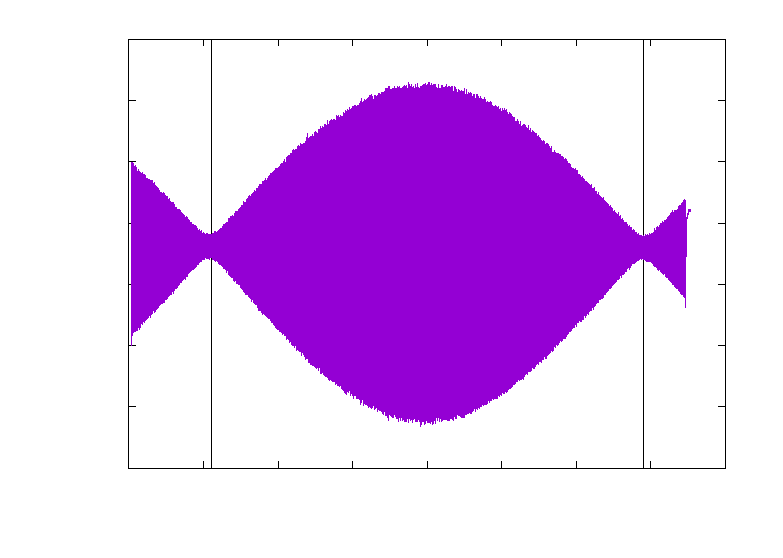
\includegraphics[width={360.00bp},height={252.00bp}]{Dominik/schwebung_na}}%
    \gplfronttext
  \end{picture}%
\endgroup
}
    \caption{Aufnahme der Schwebung des Interferogramms der Na-D Linie mit eingezeichneten Minima (Knoten)}
\end{figure}\\
Der Abstand zwischen zwei Knoten der Schwebung beträgt:
\begin{equation}
    \Delta S=\left(0,290\pm0,005\right)\,\text{mm}%8,295-8,005
\end{equation}
Dieser kann genutzt werden, um den Wellenlängenabstand der beiden Schwebungswellenlängen zu berechnen:%Minimas in der Schwebung werden erreicht für:
\begin{align}
    \cos\left(\Delta kl\right)&=0\\
    \Delta kl&=\frac{\left(2n-1\right)\pi}{2}\\
    \Delta k&=\frac{\left(2n-1\right)\pi}{2l}
\end{align}
Da wir einen 'Bauch' der Schwebung betrachten folgt: $l=S/2$ und $n=1$\\
Somit folgt für den Wellenlängenabstand der Schwebung im l-Raum:
\begin{align}
    \Delta k&=\frac{\pi}{S}\\
    \Delta \lambda&=\frac{\lambda_{Na}^2}{2S}\\
    \Delta \lambda&=\left(0,594\pm0,006\right)\,\text{nm}
\end{align}
Betrachten wir den Abstand zwischen den Literaturwerten für die Natrium D-1 und D-2 Linie $(\Delta\lambda=0,597\,\text{nm})$, so sehen wir, dass wir mit der Messung und dem Fehler diesen Wert einschließen.\\
Für die Amplitude einer Schwebung folgt aus den Fragen zur Vorbereitung:
\begin{equation}
    A=\sqrt{A_1^2+A_2^2+2A_1A_2\cos(\left|\omega_2-\omega_1\right|t)}
\end{equation}
Somit folgt für die Intensität im Knoten (Minima):
\begin{equation}
    A_K=\sqrt{A_1^2+A_2^2-2A_1A_2}=A_1-A_2
\end{equation}
Für die Intensität im Bauch (Maxima) folgt:
\begin{equation}
    A_B=A_1^2+A_2^2+2A_1A_2=A_1+A_2
\end{equation}
Wenn man nun das Intensitätsverhältnis/Amplitudenverhältnis $A_2/A_1$ haben möchte, kann man dies durch lösen des LGS bekommen:
\begin{equation}
    \frac{A_2}{A_1}=\frac{A_B-A_K}{A_B+A_K}
\end{equation}
Somit folgt für das gemessene Verhältnis (Ablesefehler: $0,001\,\text{V}$): %offset:0,325
\begin{equation}
    \frac{A_2}{A_1}=\left(0,875\pm0,002\right)%0,037_K/0,554_B
\end{equation}
Als Literaturwert wurde der Wert $0,8$ gefunden \citep[vgl.][S. 92]{Zusatzliteratur}.
Unser berechneter Wert schließt den theoretisch zu erwarteten Wert zwar nicht ein, liegt dennoch in dessen Größenordnung.
\subsection{Verbreiterungsmechanismus der Lampe}
Wie schon im vorherigen Teil zur Linienbreite gesagt wurde, ist die Natriumdampflampe doppelverbreitert.
Dies erkennt man daran, dass die Einhüllende des Interferogramms gaußförmig ist und nicht einer beidseitig abfallenden e-Funktion ähnelt.\\
Die Doppelverbreiterung kommt daher, dass die Lampe eine sehr hohe Betriebstemperatur von mehreren hundert Grad hat \citep[vgl.][]{Na-Dampf-Wiki}.
Durch die hohen Temperaturen dominiert die Doppelverbreiterung in Vergleich zur Druckverbreiterung.
\begin{figure}[h]
    \centering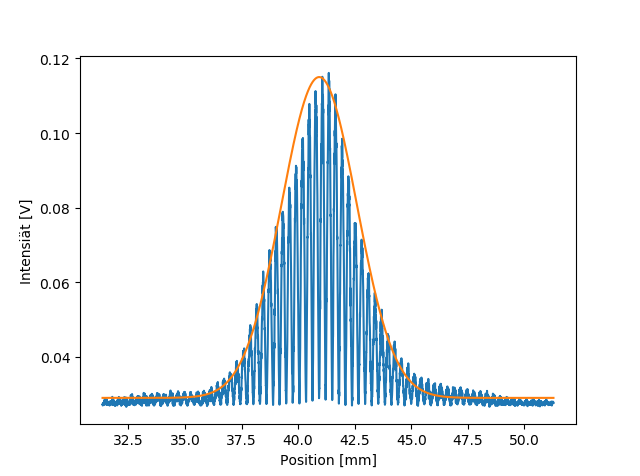
\includegraphics[width=0.8\textwidth]{Dominik/neu.png}
    \caption{Einhüllende des Interferogramms der Na-D Linie mit eingezeichnetem Gaußfit}
    \label{abbildung_ein}
\end{figure}
\newpage\newpage
\section{Donoremission nach Akzeptorbleichen}
In diesem Versuchsteil soll die FRET-Effizienz an CFP/YFP markierten Zellen bestimmt werden, indem 
die Donorfluoreszenz vor und nach dem Photobleaching des Akzeptormoleküls gemessen wird. \\
Während dem Bleichvorgang wird (idealerweise) nur der Akzeptor mit einem Laser der Wellenlänge 514 nm bei 
100\% Intensität bestrahlt und somit wird die Fluoreszenz des Akzeptors YFP verringert. \\
Während dem Versuch werden erst 10 Bilder vor dem Bleichen aufgenommen. Im nächsten Schritt
werden weitere 5 Bilder aufgenommen, diese stellen den Bleichvorgang dar. Zuletzt werden noch einmal 10 Bilder aufgenommen, 
um die Zelle nach dem Bleichvorgang auswerten zu können.\\
Um aus diesen Bildern die mittleren Intensitäten mithilfe des Messprogramm zu bekommen, werden sogenannte \textit{region of interest} (ROI) bestimmt. 
Die erste ROI 1 enthält immer den vollständig bestrahlten Bereich der Zelle während dem Bleichvorgangs. 
Die zweite ROI 2 wird um die Membran gezogen. 
Bei der dritten ROI 3 wird ein Ort in der Zelle gewählt, der sich durch besonders hohe Fluoreszenz auszeichnet. Bei einigen  
Messungen kam es hierbei allerdings zu einer unterschiedlichen Anzahl von ROI 3. Damit die 
verschiedenen Zellen besser vergleichbar sind,
wurden die ROI jeweils nach dem oben beschrieben Kriterien ausgewählt.\\
Um die ROI zu verdeutlichen, soll die folgende Graphik als Beispiel für die aufgenommenen Bilder
während dem Versuch dienen.\\
\begin{figure}[h]
    \centering
    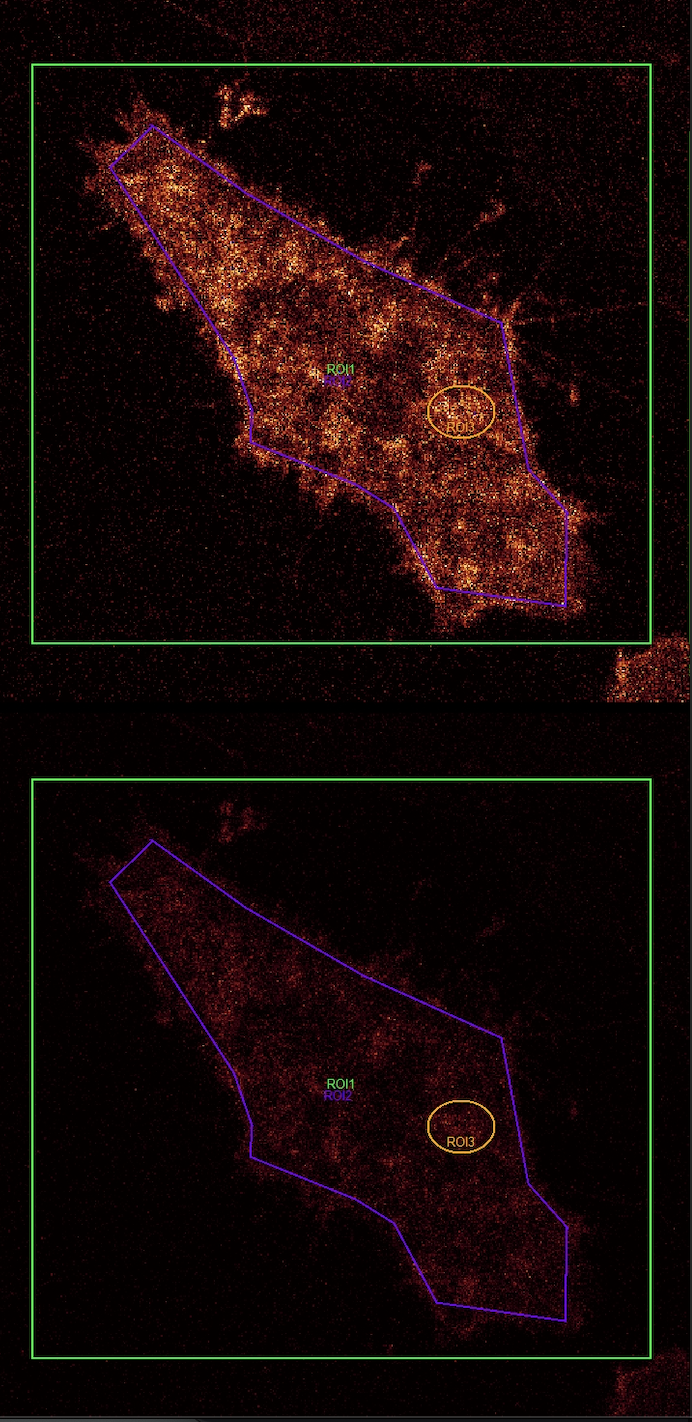
\includegraphics[scale=0.5]{Bilder/Auswertung_Anna/beispiel.PNG}
    \caption{Zelle 06 der YFP/CFP Probe vor und nach dem Bleichvorgang, unterteilt in verschiedenen ROI.}
    \label{fig:Beispeil}
   \end{figure}
\newpage
Das erste Bild steht hierbei für die Aufnahme vor dem Photobleaching und das zweite zeigt eine Aufnahme danach.
An diesen Bildern erkennt man die oben beschrieben ROI. Das grüne Rechteck steht für die ROI 1, die pinke Ummantelung für ROI 2
und der orangene Kreis für ROI 3, einen Bereich mit hoher Fluoreszenz innerhalb der Membran. \\\\
Zuerst wurden die Proben mit CFP und YFP markierten Zellen untersucht, anschließend
die nur CFP Proben und zuletzt die YFP Proben. Bei den ersten beiden Versuchsteilen wurde die 
Donorintensität betrachtet, im letzten Schritt allerdings die Akzeptorintensität. 
Nach der Mittelwertbildung wurden noch die Verhältnisse gebildet, um einen Vergleich 
ziehen zu können.
\subsection{CFP und YFP Proben}
Hier wurden zuerst über die Donorintensität $D_{CY,pre}$ vor der Akzeptorbleichung  
und die Donorintensität $D_{CY,post}$ nach dem Bleichvorgang für jede einzelne Zelle gemittelt. Anschließend 
wird die FRET-Effizienz E nach der im Skript angegeben Formel berechnet:
\begin{equation}
    E = 1 - \frac{D_{CY,pre}}{D_{CY,post}}
\end{equation}
Aus der folgenden Tabelle sind die entsprechenden Werte zu entnehmen:\\
\begin{table}[h]
    \centering
      \begin{tabular}{c|c|c|c}
      \textbf{Zelle} & \textbf{ROI 1} & \textbf{ROI 2} & \textbf{ROI 3} \\
      \hline
      \textbf{1} & 0,02  & 0,03  & 0,04 \\
      \textbf{2} & 0,02  & 0,04  & 0,07 \\
      \textbf{3} & 0,07  & 0,01  & 0,11 \\
      \textbf{4} & 0,04  & 0,07  & 0,13 \\
      \textbf{5} & 0,01  & 0,02  & -0,01 \\
      \textbf{6} & 0,10  & 0,10  & 0,06 \\
      \textbf{7} & -0,02 & -0,01 & 0,07 \\
      \textbf{8} & 0,01  & 0,03  & 0,07 \\
      \end{tabular}
      \caption{FRET-Effizienz, berechnet aus der Donorintensitäten (von CFP/YFP Proben) vor und nach dem Bleichvorgang für 8 Zellen.}
    \label{tab:FRET-Effizienz}
  \end{table}\\
Hierbei muss gesagt werden, dass die aufgeführten Werte nicht die kompletten Werte der Messung sind. 
Die erste Messung wurde in dieser Tabelle nicht mit aufgeführt, da hierbei nur zwei ROI gemessen wurden und 
somit der Vergleich der dritten ROI nicht gegeben war. Die dritte Messung wurde ebenfalls ausgeschlossen, 
da auch hier nur zwei ROI gemessen wurden. 
Die letzten Messungen wurden hier ebenfalls ausgelassen, da bei diesen Messungen nur die 
halbe Zelle gebleicht wurde. \\
Wenn man nun die verbliebenen Messungen betrachtet, fällt wie erwartet auf, dass 
ROI 1 die geringste Effizienz aufweist. Dies hat den Grund, dass dieses Gebiet nicht nur
die Zelle beinhaltet, sondern auch 'toten Raum', in diesem Raum befinden sich keine 
fluoreszierende Punkte. Ein 'Ausreißer' ist hier die Zelle 3, dies hat wahrscheinlich den Grund, 
dass bei unserer Aufnahme das Gebiet aus zwei Zellen besteht und nicht nur aus einer. \\
Allgemein fällt noch auf, dass die Werte sehr klein sind, dies kann man darauf zurückführen, dass die
Akzeptorbleichung nicht in der gewünschten Stärke (nach Anleitung sollten es mindestens 50\% sein) bei unserem Versuch möglich war. \\
Bei den negativen Ergebnissen kann man davon ausgehen, dass der Bleichvorgang, keine Wirkung auf 
die Zelle hatte.
\newpage
Eine deutlich höhere Effizienz hatte dabei allerdings der Bereich der Zellmembran ROI 2, da in diesem Bereich
auch eine deutlich höhere Ansammlung an CFP und YFP Proben vorliegt, diese fluoreszieren können. Somit scheint 
die höhere Effizienz, im Gegensatz zur ROI 1, plausibel.\\
Laut Theorie sollte der größte Wert der Effizienz in der ROI 3 zu finden sein, da diese auch dementsprechend gewählt wurde. 
Allerdings ist dies nicht immer der Fall, dies lässt sich auf die Tatsache zurückführen, 
dass die ROI 'per Auge' von uns während dem Versuch ausgewählt wurde und somit nicht garantiert werden kann, dass
es sich bei ROI 3 wirklich um das Gebiet mit der stärksten Bleichung handelt.\\\\
In dem folgenden Diagramm \ref{fig:plotA2} wird die Fluoreszenzintensität des Donors und des S.E. Channels 
gegen die Zeit aufgetragen. Dies wird beispielhaft an einer Zelle (Zelle 03) dargestellt und nur für die ROI 1.
Die grüne Linie beschreibt hierbei die Donorintensität. Diese Linie verläuft am Anfang
beinahe horizontal, dies ist die Zeit vor dem Bleichen. Während dem Photobleaching 
hat die CFP Probe keine Intensität, da diese bei dem Bleaching (idealerweise) auch nicht bestrahlt
wird. Es soll lediglich das Akzeptormoleküls gebleicht werden.
Nach der 'Lücke' ist die Linie wieder eine Gerade (parallel zur x-Achse), diese stellt den Zeitraum
nach dem Bleaching dar. \\
Die blaue Linie in der Grafik zeigt die Sensitized Emission. Wie man erkennen kann, 
verläuft diese ebenfalls parallel zur x-Achse vor dem Bleaching, allerdings fällt auf, 
dass die Intensität der S.E. Probe deutlich höher liegt als die zu vergleichende
Probe. Während dem Photobleaching steigt die blaue Linie sprunghaft an, 
dies ist plausibel, wenn man bedenkt, dass der Akzeptor mit voller 
Laser Intensität bestrahlt wird. Zuletzt sinkt die 
Linien wieder und setzt sich wieder als Gerade fort, da sich die Intensität 
nach dem Photobleaching nicht mehr großartig ändert.\\
Beide Intensitäten sind allerdings vor dem Bleaching höher als nachdem, dies entspricht den Erwartungen.\\
\begin{figure}[h]
\centering
  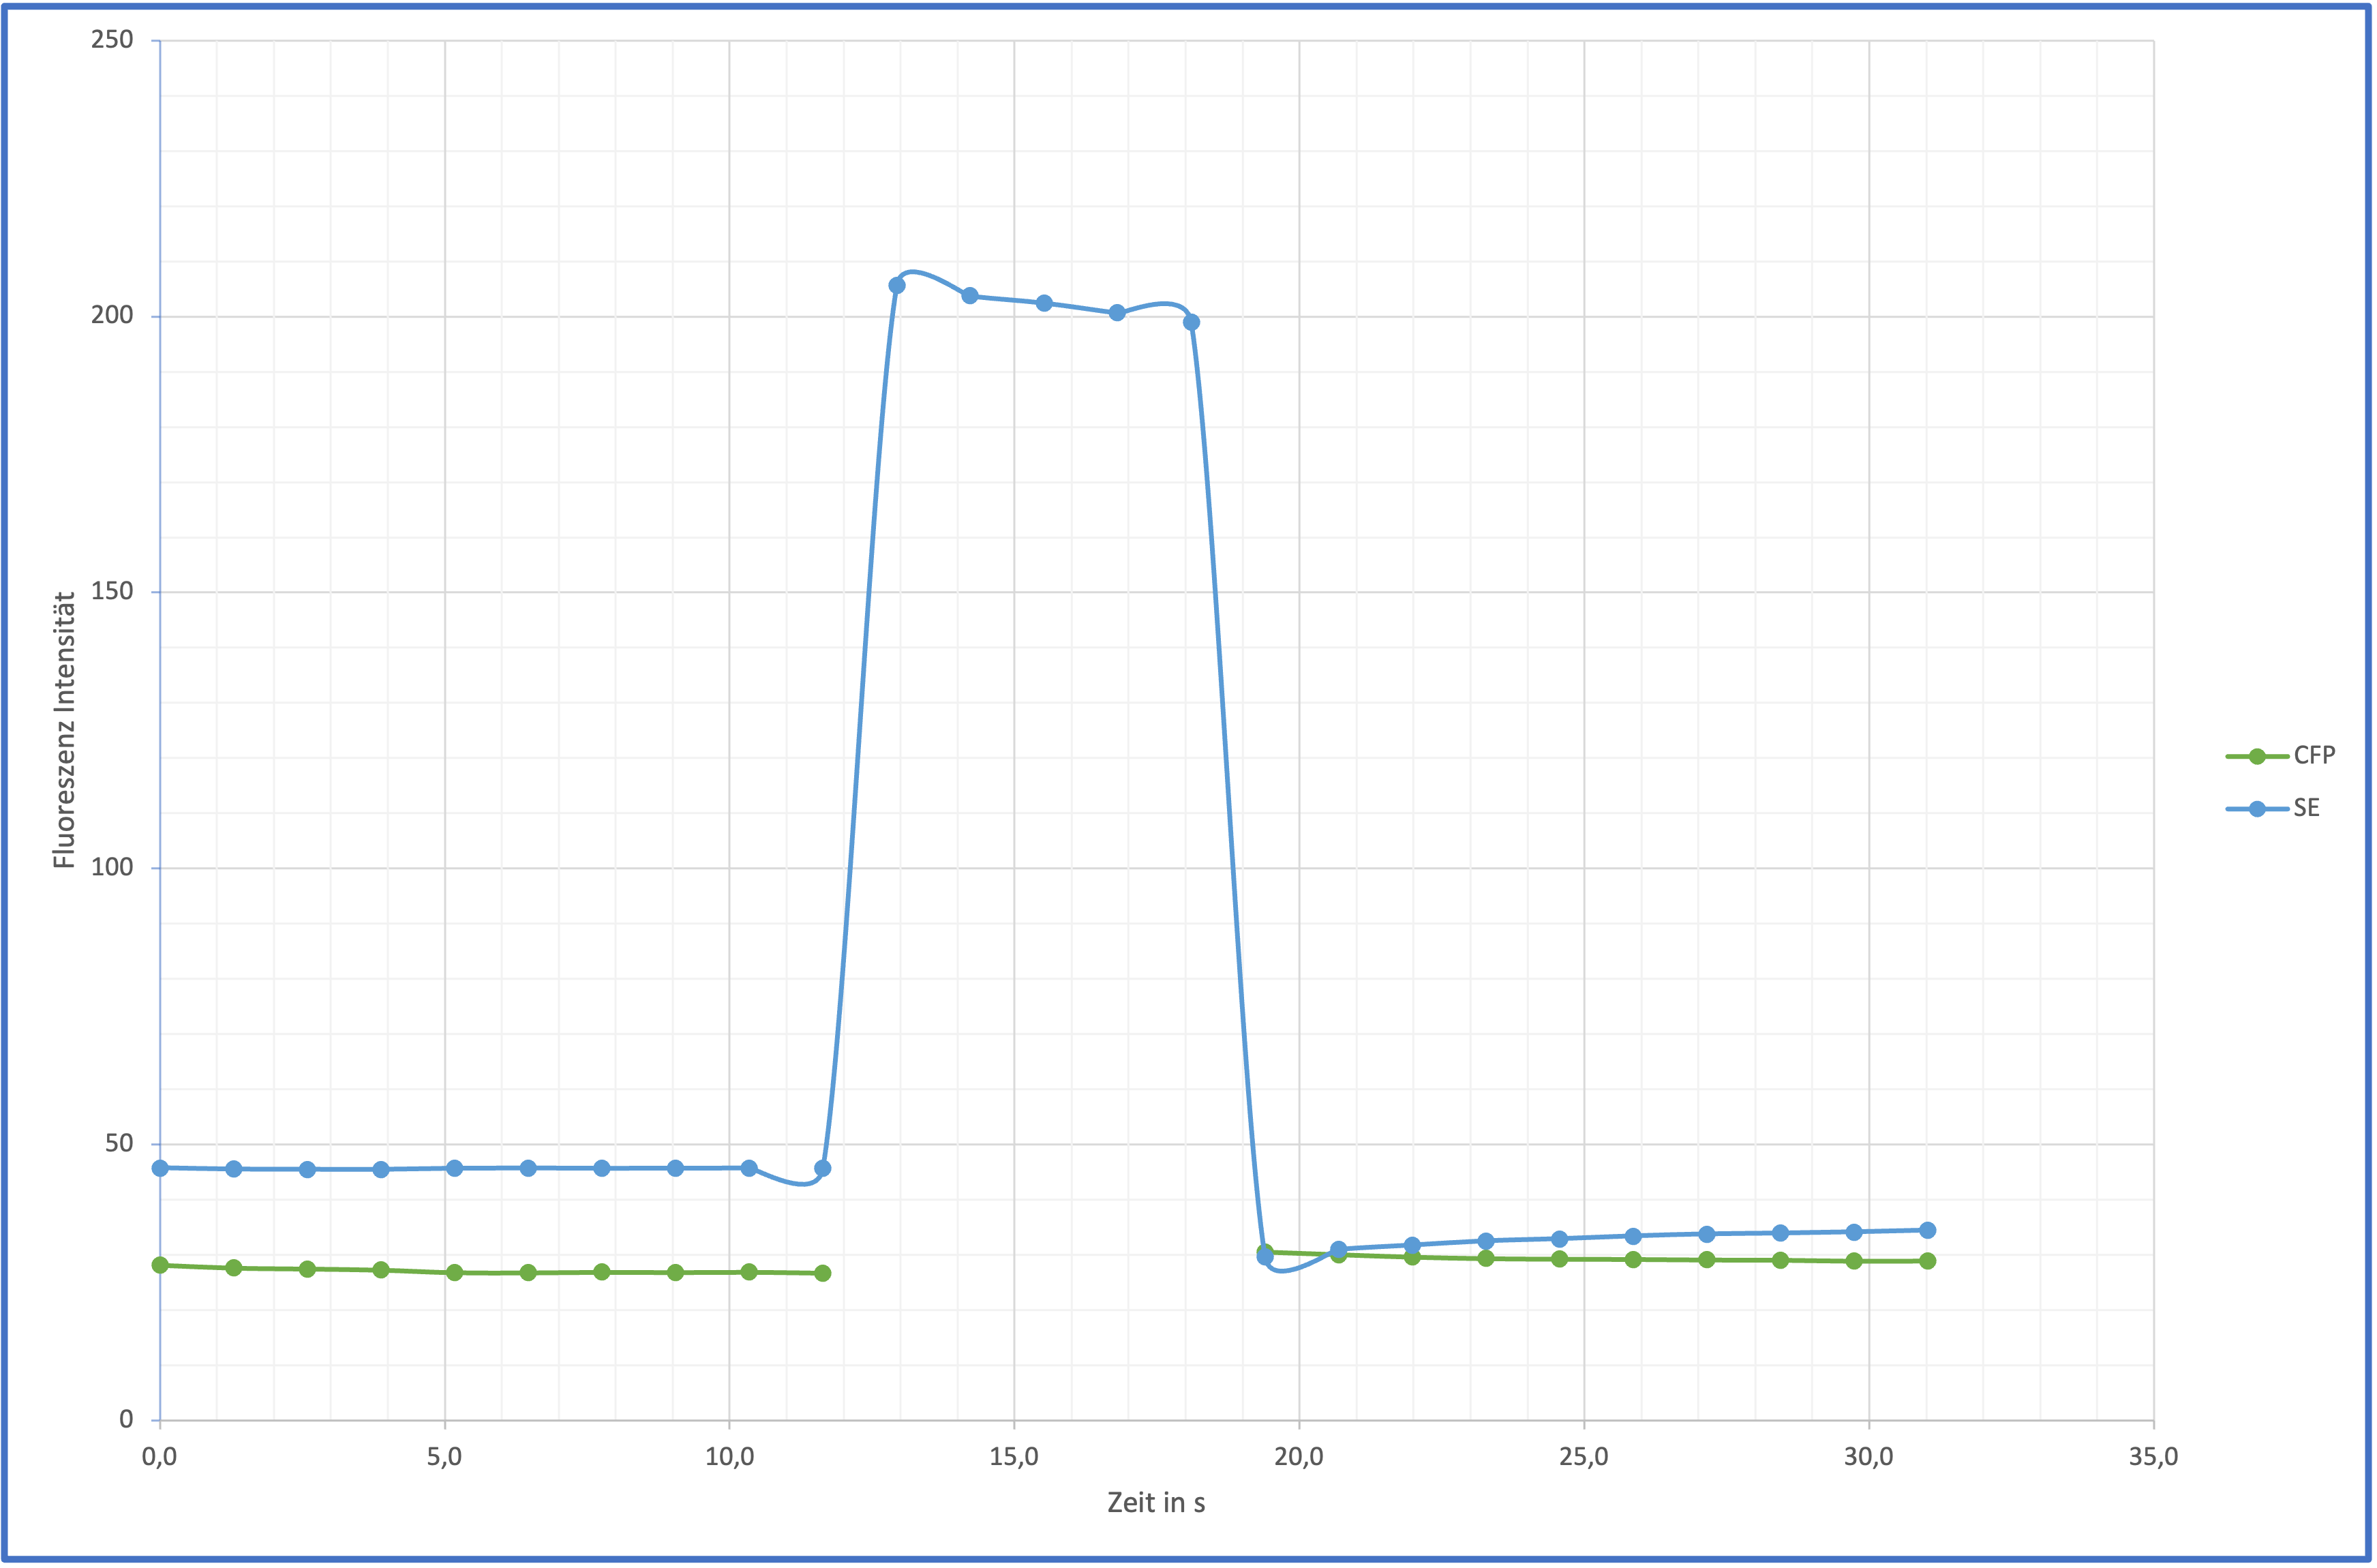
\includegraphics[scale=0.3]{Bilder/Auswertung_Anna/plot.PNG}
  \caption{Grafik über die Fluoreszenz Intensität vor, während und nach dem Photobleaching über einen Zeitraum. Blau: Sensitized Emission; Grün: Donorintensität}
  \label{fig:plotA2}
\end{figure}\\
\subsection{CFP-Proben}
Desweitern wurde die Akzeptorbleichung nur bei CFP-Proben aufgenommen, um einen Kontrollpunkt zu bekommen. 
Laut Theorie sollte es hier keinen Unterschied zwischen der Intensität vor und nach dem Bleichvorgang 
geben. Um dies zu untersuchen wird das folgende Verhältnis gebildet:
\begin{equation}
    V_1 = \frac{D_{CY,pre}}{D_{CY,post}}
\end{equation}
\newpage
Die Werte sind in der folgenden Tabelle aufgeführt:
\begin{table}[h]
    \centering
      \begin{tabular}{c|c|c|c}
      \textbf{Zelle} & \textbf{ROI 1} & \textbf{ROI 2} & \textbf{ROI 3} \\
      \hline
      \textbf{1} & 1,02  & 0,99  & 1,00 \\
      \textbf{2} & 1,03  & 1,02  & 1,09 \\
      \textbf{3} & 1,02  & 1,01  & 1,01 \\
      \textbf{4} & 1,01  & 1,01  & 1,05 \\
      \textbf{5} & 1,02  & 1,02  & 0,97 \\
      \textbf{6} & 1,00  & 1,01  & 1,02 \\
      \textbf{8} & 1,00  & 1,03  & 0,98 \\
      \textbf{9} & 1,03  & 0,89  & 1,04 \\
      \textbf{10} & 1,03  & 0,03  & 1,04 \\
      \textbf{11} & 1,00  & 1,03  & 1,01 \\
      \end{tabular}
      \caption{Verhältnis der Donorintensitäten einer reiner CFP Probe vor und nach der Bleichung für 3 ROI für je 11 Zellen.}
    \label{tab:Verhältnis CFP}
  \end{table}\\
  Wie man erkennt, stimmt die Theorie ziemlich gut mit dem Experiment überein, da die Werte nahe um 1 
  liegen. Das bedeutet, dass während dem Photobleaching zum größtenteils nur der Akzeptor gebleicht wurde.
\subsection{YFP-Proben}
Zuletzt wurde das Akzeptorbleichen auch auf reine YFP Proben angewendet. 
Hierbei wurde allerdings das Verhältnis der Akzeptorintensitäten vor und nach dem Bleaching betrachtet
und ins Verhältnis versetzt. 
\begin{equation}
    V_2 = \frac{A_{YFP,post}}{A_{YFP,pre}}
\end{equation}
Die Werte finden sich in der folgenden Tabelle:
\begin{table}[h]
    \centering
      \begin{tabular}{c|c|c}
      \textbf{Zelle} & \textbf{ROI 1} & \textbf{ROI 2} \\
      \hline
      \textbf{1} & 0,39  & 0,49 \\
      \textbf{2} & 0,38  & 0,46 \\
      \textbf{3} & 0,44  & 0,47 \\
      \textbf{4} & 0,71  & 0,67 \\
      \textbf{5} & 0,35  & 0,33 \\
      \textbf{6} & 0,29  & 0,38 \\
      \end{tabular}
      \caption{Verhältnis der Akzeptorintensitäten vor und nach dem Bleichvorgang einer reinen YFP Probe für 6 Zellen.}
    \label{tab:Verhältnis der Akzeptorintensitäten}%
  \end{table}%
  
Theoretisch sollte die Intensität nach dem Photobleaching deutlich geringer ausfallen, also davor. 
 Wie man erkennen kann, ist dies auch der 
Fall, allerdings fällt die Stärke des Photobleaching deutlich geringer aus als gefordert.\\\\
Zuletzt soll dieses Verfahren noch mit der vorangegangenen Methode verglichen werden. Die FRET-Effizienz Werte
der Sensitized Emission liegen deutlich höher (vgl. Tabelle \ref{tab:SE Effizienz}), als die Werte der FRET Effizienz der Akzeptorbleichung. \\
Ein generelles Problem, welches zu hohen Messunsicherheiten führt, ist das die ROI willkürlich während dem 
Versuch bestimmt werden. Ein Problem dieser Messmethode (Akzeptorbleaching) ist, dass nur ein Teil des YFP 
Moleküls gebleicht wird, wie die Tabelle \ref{tab:Verhältnis der Akzeptorintensitäten} zeigt. Dies 
führt zu dieser großen Abweichung der FRET Effizienz zwischen den verschiedenen Messmethoden.
\newpage
\section{Lebenszeitmessungen}
	In diesem Versuchsteil soll die Lebenszeit von Zellen, die sich im angeregten Zustand befinden, ermittelt werden. Die Zellen sind dabei entweder mit CFP oder YFP bzw. mit CFP und YFP markiert. Der hierzu verwendete Laser ist ein gepulster $470\,$nm Laser mit einer Frequenz von $40\,$MHz. Zudem wurden noch zwei Avalanche-Photodioden mit entsprechenden Filterwürfeln benutzt. Wie dem Skript zu entnehmen ist, werden in Kanal 1 hauptsächlich CFP-Emissionen detektiert, wobei in Kanal 2 größtenteils YFP-Emissionen gemessen werden. Am Anfang des Versuchs wurde zunächst die instrument response function (kurz: IRF) gemessen. Dabei ergab sich folgendes Bild:
	\begin{figure}[h]
		\centering
		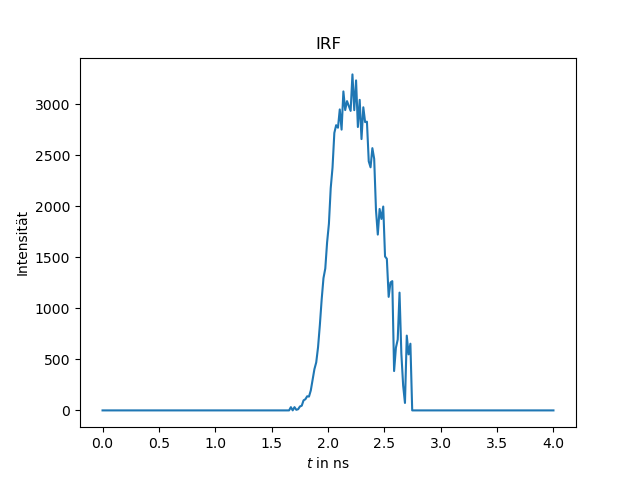
\includegraphics[width=7cm,height=5cm]{Auswertung-David/IRF-plot}
		\caption{Im Experiment gemessene IRF}
		\label{IRF}
	\end{figure}\\
	Anschließend wurde die Anzahl an detektierten Photonen über einem Zeitraum von ca. 2 Minuten gemessen und in Form eines Histogramms visualisiert. Das Histogramm einzelmarkierten Zellen wurde - im Bereich des exponentiellen Abfalls - durch einen single exponential fit genähert. Im Folgenden sind zwei Beispiele der daraus entstandenen Plots zu sehen.\\
	\begin{figure}[h]
		\begin{minipage}{.4\linewidth} % [b] => Ausrichtung an \caption
			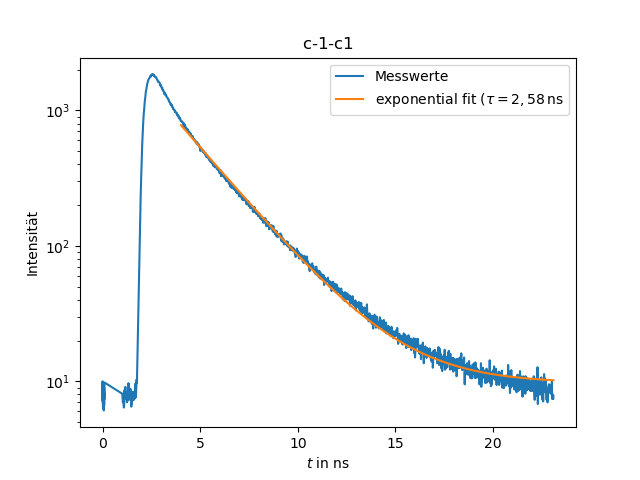
\includegraphics[width=\linewidth]{Auswertung-David/c-1-c1-plot}
			\caption{CFP-Signal in Kanal 1}
		\end{minipage}
		\hspace{.1\linewidth}% Abstand zwischen Bilder
		\begin{minipage}{.4\linewidth} % [b] => Ausrichtung an \caption
			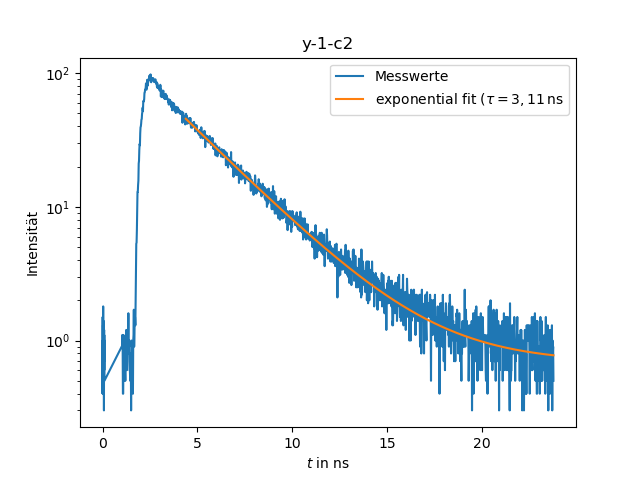
\includegraphics[width=\linewidth]{Auswertung-David/f-1-c2-plot}
			\caption{YFP-Signal in Kanal 2}
		\end{minipage}
	\end{figure}\\
Dadurch ergaben sich folgende Werte für die Lebenszeiten $\tau_{CFP}$ und $\tau_{YFP}$:\\
\begin{center} 
\begin{tabular}[c]{ccc}
	\hline
	 & $\tau_{CFP}$ in ns & $\tau_{YFP}$ in ns \\
	\hline
	Messung Nr. 1 & $2,58$ & $3,11$ \\
	Messung Nr. 2 & $2,51$ & $3,06$\\
	Messung Nr. 3 & $2,57$ & $3,03$\\
	\hline
	mittlere Lebensdauer & $2,55$ & $3,07$\\
	\hline
\end{tabular}\\
\end{center}
\newpage
Für die Bestimmung der Lebenszeiten der doppelt markierten Zellen wurde ein double exponential fit mit folgendem Ansatz genutzt:\\
\begin{equation}
N(t) = A_{1} \mathrm{e}^{-\frac{t}{\tau_1}}+A_{2} \mathrm{e}^{-\frac{t}{\tau_2}}
\end{equation}
Eine kleine Auswahl der Plots sah wie folgt aus:\\
\begin{figure}[h]
	\begin{minipage}{.4\linewidth} % [b] => Ausrichtung an \caption
		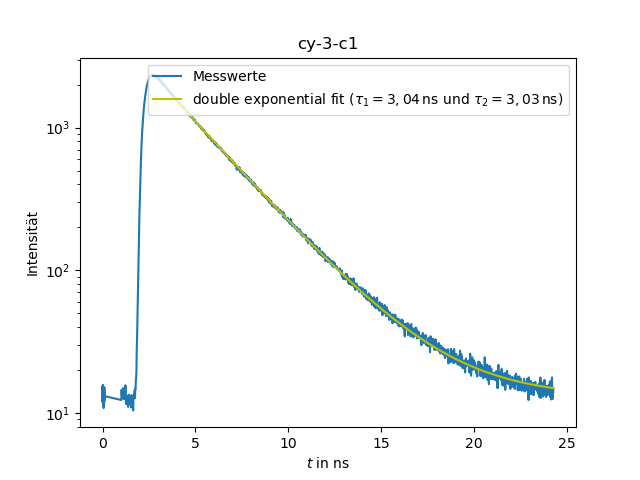
\includegraphics[width=\linewidth]{Auswertung-David/cy-3-c1-plot}
		\caption{CFP/YFP-Signal in \\Kanal 1}
	\end{minipage}
	\hspace{.1\linewidth}% Abstand zwischen Bilder
	\begin{minipage}{.4\linewidth} % [b] => Ausrichtung an \caption
		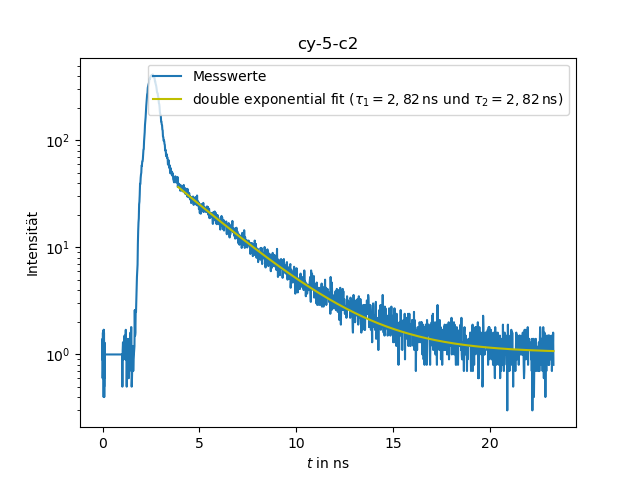
\includegraphics[width=\linewidth]{Auswertung-David/cy-5-c2-plot}
		\caption{CFP/YFP-Signal in \\Kanal 2}
	\end{minipage}
\end{figure}\\
Das Vorgehen zur Bestimmung der Lebenszeiten erfolgte analog zu oben und ergab folgende Werte:\\
\begin{center} 
	\begin{tabular}[c]{ccc}
		\hline
		& $\tau_{\mathrm{Kanal 1}}$ in ns & $\tau_{\mathrm{Kanal 2}}$ in ns \\
		\hline
		Messung Nr. 1 & $2,31$ & $2,94$ \\
		Messung Nr. 2 & $3,00$ & $2,66$ \\
		Messung Nr. 3 & $3,04$ & $2,83$ \\
		Messung Nr. 4 & $2,97$ & $2,86$ \\
		Messung Nr. 5 & $3,01$ & $2,82$ \\
		\hline
		mittlere Lebensdauer & $2,87$ & $2,82$\\
		\hline
	\end{tabular}\\
\end{center}
Hieraus lässt sich nun die FRET-Effizienz bestimmen:\\
\begin{equation}
E = 1-\frac{\tau_{CFP,\:FRET}}{\tau_{CFP,\:no\:FRET}}=-0,13
\end{equation}
Es fällt sofort auf, dass die Lebenszeit ohne FRET kleiner ist, als die Lebenszeit mit FRET, was zu einer negativen FRET-Effizienz führt und das wiederum ist physikalisch nicht möglich. \\
Im letzten Abschnitt dieses Versuchsteils soll die Messkurve durch eine Faltung der IRF mit einem exponential fit angenähert werden.\\
\newpage
Hierbei ergab sich folgendes Bild:\\
\begin{figure}[h]
	\centering
	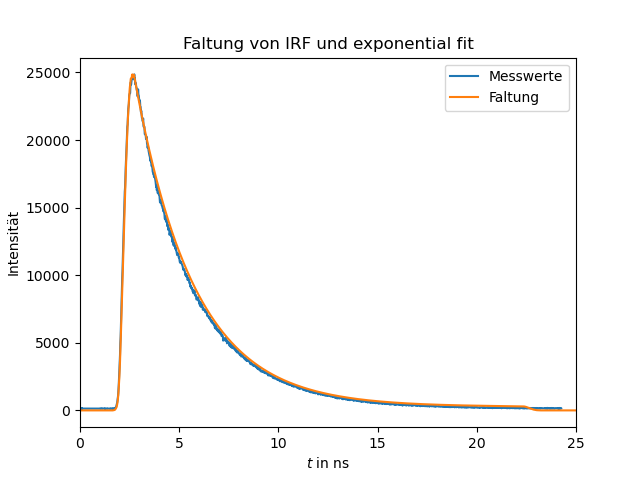
\includegraphics[width=9cm,height=7cm]{Auswertung-David/faltung-plot}
	\caption{Faltung der genäherten Exponentialfunktion mit der im Experiment ermittelten IRF}
	\label{Faltung von IRF und Exponentialfkt.}
\end{figure}\\
Anschließend wird die Exponentialfunktion noch mit einem Gauß-Fit der IRF gefaltet.  Für den Gauß-Fit ergaben sich eine Standardabweichung von $\sigma=0,21\,\mathrm{ns}$ und ein Erwartungswert von $\mu=2,26\,\mathrm{ns}$, woraus sich folgender Graph bestimmen ließ:
\begin{figure}[h]
	\centering
	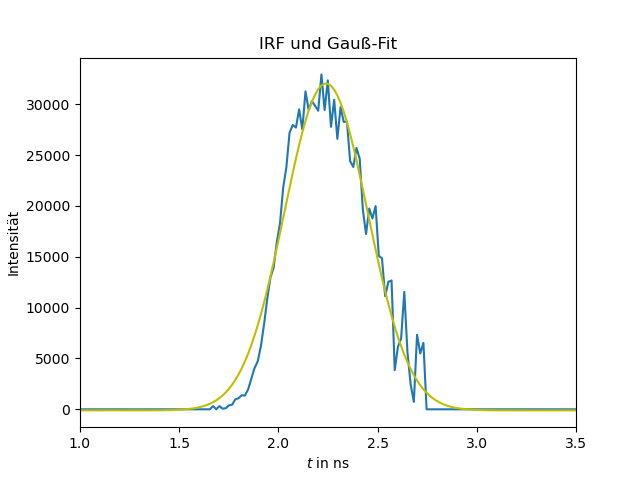
\includegraphics[width=9cm,height=7cm]{Auswertung-David/Gauss-fit-plot}
	\caption{Durch Gauß-Funktion genäherte IRF}
	\label{Gauss-Fit}
\end{figure}\\
\newpage
Durch die Faltung mit Gauß-Funktion und IRF entstand dieses Bild:
\begin{figure}[h]
	\centering
	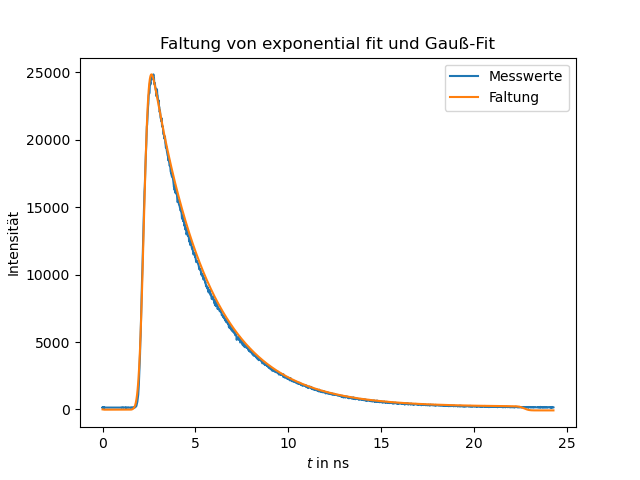
\includegraphics[width=9cm,height=7cm]{Auswertung-David/faltung-gauss-plot}
	\caption{Faltung von Gauß- und Exponentialfunktion}
	\label{Faltung mit Gauss-Fit}
\end{figure}\\
Die durch Faltung entstandene Funktion musste in beiden Fällen noch normiert werden, da bei der Faltung die Vorfaktoren - der miteinander gefalteten Funktionen - multipliziert wurden und die Faltung somit einige Größenordnungen über den Messwerten lag. Es fällt sofort auf, dass sich die Faltungen sehr gut an die Messkurve annähern und sich das Messsignal somit, durch die Faltung, ziemlich genau rekonstruieren lässt.
\newpage
\subsection{Abweichungen von Daten und Fits}
\begin{figure}[h]
	\centering
	\subfigure[Abweichung von Messwerten und Fit (cy-3-c1), berechnet mit np.cumsum($(y_{data}-y_{fit})^2$)]{
		\centering
		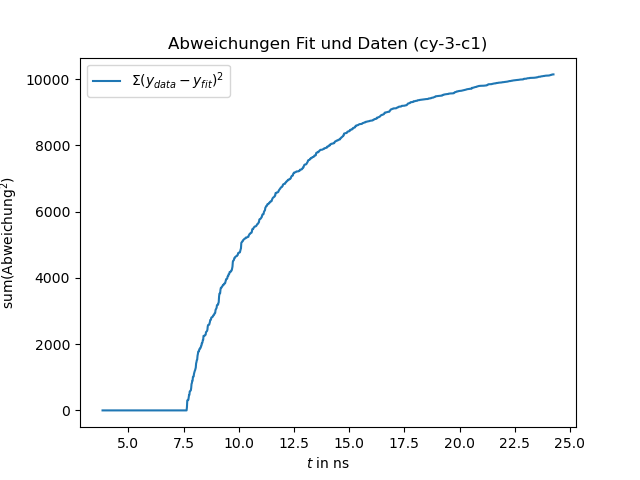
\includegraphics[width=0.3\textwidth]{Auswertung-David/Abweichungen_double_exp_fit_und_Daten_(cy-3-c1)}
		\label{fig:cy3c1}
	}
	\hfill
	\subfigure[Abweichung von Messwerten und Fit (cy-5-c2), berechnet mit np.cumsum($(y_{data}-y_{fit})^2$)]{
		\centering
		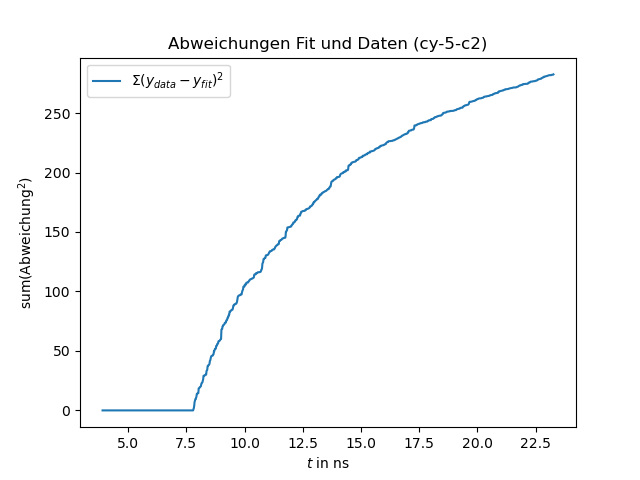
\includegraphics[width=0.3\textwidth]{Auswertung-David/Abweichungen_double_exp_fit_und_Daten_(cy-5-c2)}
		\label{fig:cy5c2}
	}
	\hfill
	\subfigure[Abweichungen von Faltung (IRF und Exp.) und Daten, berechnet mit np.cumsum($(y_{data}-y_{fit})^2$)]{
		\centering
		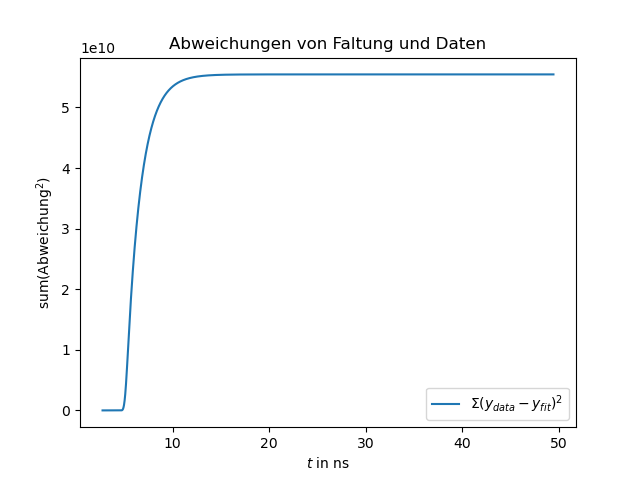
\includegraphics[width=0.3\textwidth]{Auswertung-David/Abweichungen_Faltung_und_Data}
		\label{fig:expIRF}
	}
	\hfill
	\subfigure[Abweichungen von Faltung (IRF und Gaußfkt.) und Daten, berechnet mit np.cumsum($(y_{data}-y_{fit})^2$)]{
		\centering
		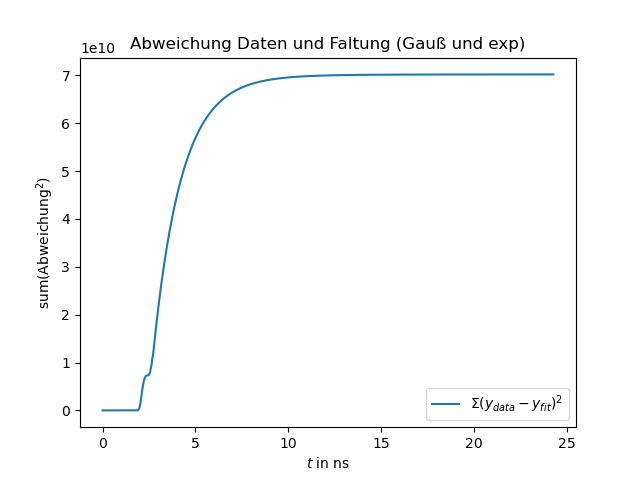
\includegraphics[width=0.3\textwidth]{Auswertung-David/Abweichungen_Gauss-Faltung_und_Data}
		\label{fig:gaussIRF}
	}
	\caption{Graphen der Summen der Abweichungen von Messwerten und Fits}
	\label{fig:abweichung}
\end{figure}

%Fazit
% 5. Einleitung

\chapter{Fazit}
\label{chap:fazit}
Alles in allem haben wir in diesem Versuch die Grundlagen der Rasterelektronenmikroskopie erlernen und anwenden dürfen. Dazu gehören die verschiedenen Detektoren und Einstellungsmöglichkeiten sowie die qualitative Analyse der aufgenommenen Bilder.\\
Unser gesammeltes Wissen wurde durch das ermitteln der Bruchursache nochmal gut gefestigt und uns wurde der Nutzen einer solchen Analyse in der Industrie klar deutlich. Auch wurde uns der Umgang mit biologischen Proben in diesem Versuch nahe gebracht, was uns in näherer Zukunft bestimmt zu gute kommen wird. Weiterhin finden wir es faszinierenden wie viel Struktur in einer so kleinen Welt noch zu finden ist und sin auch sehr überrascht, wie genau die Produktion eines Micro-Chips sein muss, um die Fertigung solch kleiner Schaltkreise zu ermöglichen.\\

Abschließen ist zu bemerken, dass der Versuch als Erfolg zu verbuchen ist, da er uns Praxisnah den Umgang mit einer der wichtigsten Untersuchungsmethoden vertraut gemacht hat.
\appendix
%Messprotokoll

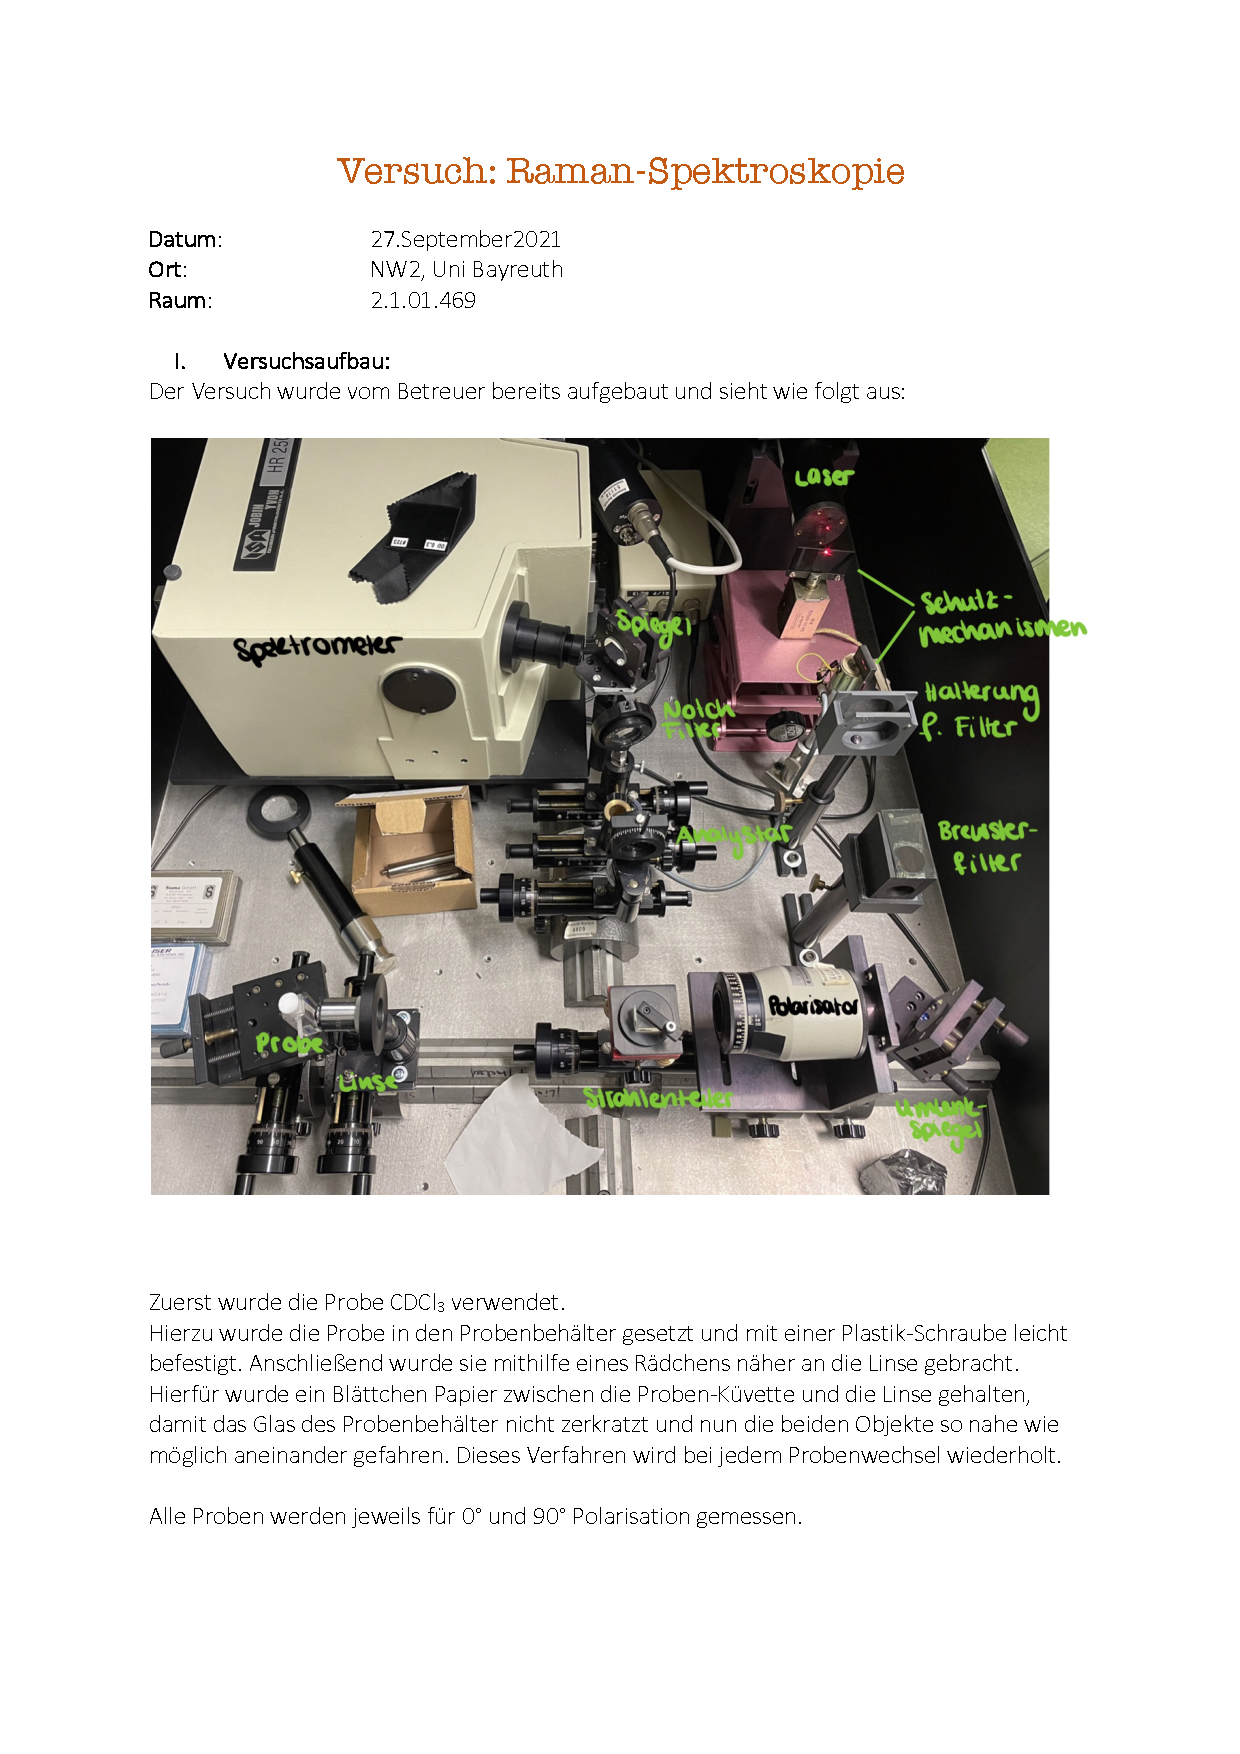
\includepdf[pages=1,landscape = false, offset=0 -25mm, scale=0.71,pagecommand ={\thispagestyle{empty}}\chapter{Messprotokoll}]{Protokoll_Messung/Protokoll.pdf}

\includepdf[pages={2-4},scale=0.8,pagecommand ={\thispagestyle{plain}}]{Protokoll_Messung/Protokoll.pdf}
\chapter{Gemessene Plots}
\section{Tetrachlormethan}
\begin{figure}[h]
    \centering\subfigure[Stokes Linien]{\scalebox{0.9}{% GNUPLOT: LaTeX picture with Postscript
\begingroup
  % Encoding inside the plot.  In the header of your document, this encoding
  % should to defined, e.g., by using
  % \usepackage[cp1252,<other encodings>]{inputenc}
  \inputencoding{cp1252}%
  \makeatletter
  \providecommand\color[2][]{%
    \GenericError{(gnuplot) \space\space\space\@spaces}{%
      Package color not loaded in conjunction with
      terminal option `colourtext'%
    }{See the gnuplot documentation for explanation.%
    }{Either use 'blacktext' in gnuplot or load the package
      color.sty in LaTeX.}%
    \renewcommand\color[2][]{}%
  }%
  \providecommand\includegraphics[2][]{%
    \GenericError{(gnuplot) \space\space\space\@spaces}{%
      Package graphicx or graphics not loaded%
    }{See the gnuplot documentation for explanation.%
    }{The gnuplot epslatex terminal needs graphicx.sty or graphics.sty.}%
    \renewcommand\includegraphics[2][]{}%
  }%
  \providecommand\rotatebox[2]{#2}%
  \@ifundefined{ifGPcolor}{%
    \newif\ifGPcolor
    \GPcolorfalse
  }{}%
  \@ifundefined{ifGPblacktext}{%
    \newif\ifGPblacktext
    \GPblacktexttrue
  }{}%
  % define a \g@addto@macro without @ in the name:
  \let\gplgaddtomacro\g@addto@macro
  % define empty templates for all commands taking text:
  \gdef\gplbacktext{}%
  \gdef\gplfronttext{}%
  \makeatother
  \ifGPblacktext
    % no textcolor at all
    \def\colorrgb#1{}%
    \def\colorgray#1{}%
  \else
    % gray or color?
    \ifGPcolor
      \def\colorrgb#1{\color[rgb]{#1}}%
      \def\colorgray#1{\color[gray]{#1}}%
      \expandafter\def\csname LTw\endcsname{\color{white}}%
      \expandafter\def\csname LTb\endcsname{\color{black}}%
      \expandafter\def\csname LTa\endcsname{\color{black}}%
      \expandafter\def\csname LT0\endcsname{\color[rgb]{1,0,0}}%
      \expandafter\def\csname LT1\endcsname{\color[rgb]{0,1,0}}%
      \expandafter\def\csname LT2\endcsname{\color[rgb]{0,0,1}}%
      \expandafter\def\csname LT3\endcsname{\color[rgb]{1,0,1}}%
      \expandafter\def\csname LT4\endcsname{\color[rgb]{0,1,1}}%
      \expandafter\def\csname LT5\endcsname{\color[rgb]{1,1,0}}%
      \expandafter\def\csname LT6\endcsname{\color[rgb]{0,0,0}}%
      \expandafter\def\csname LT7\endcsname{\color[rgb]{1,0.3,0}}%
      \expandafter\def\csname LT8\endcsname{\color[rgb]{0.5,0.5,0.5}}%
    \else
      % gray
      \def\colorrgb#1{\color{black}}%
      \def\colorgray#1{\color[gray]{#1}}%
      \expandafter\def\csname LTw\endcsname{\color{white}}%
      \expandafter\def\csname LTb\endcsname{\color{black}}%
      \expandafter\def\csname LTa\endcsname{\color{black}}%
      \expandafter\def\csname LT0\endcsname{\color{black}}%
      \expandafter\def\csname LT1\endcsname{\color{black}}%
      \expandafter\def\csname LT2\endcsname{\color{black}}%
      \expandafter\def\csname LT3\endcsname{\color{black}}%
      \expandafter\def\csname LT4\endcsname{\color{black}}%
      \expandafter\def\csname LT5\endcsname{\color{black}}%
      \expandafter\def\csname LT6\endcsname{\color{black}}%
      \expandafter\def\csname LT7\endcsname{\color{black}}%
      \expandafter\def\csname LT8\endcsname{\color{black}}%
    \fi
  \fi
    \setlength{\unitlength}{0.0500bp}%
    \ifx\gptboxheight\undefined%
      \newlength{\gptboxheight}%
      \newlength{\gptboxwidth}%
      \newsavebox{\gptboxtext}%
    \fi%
    \setlength{\fboxrule}{0.5pt}%
    \setlength{\fboxsep}{1pt}%
\begin{picture}(7200.00,5040.00)%
    \gplgaddtomacro\gplbacktext{%
      \csname LTb\endcsname%%
      \put(726,440){\makebox(0,0)[r]{\strut{}$0.05$}}%
      \put(726,1316){\makebox(0,0)[r]{\strut{}$0.1$}}%
      \put(726,2192){\makebox(0,0)[r]{\strut{}$0.15$}}%
      \put(726,3067){\makebox(0,0)[r]{\strut{}$0.2$}}%
      \put(726,3943){\makebox(0,0)[r]{\strut{}$0.25$}}%
      \put(726,4819){\makebox(0,0)[r]{\strut{}$0.3$}}%
      \put(858,220){\makebox(0,0){\strut{}$560$}}%
      \put(1601,220){\makebox(0,0){\strut{}$570$}}%
      \put(2344,220){\makebox(0,0){\strut{}$580$}}%
      \put(3087,220){\makebox(0,0){\strut{}$590$}}%
      \put(3831,220){\makebox(0,0){\strut{}$600$}}%
      \put(4574,220){\makebox(0,0){\strut{}$610$}}%
      \put(5317,220){\makebox(0,0){\strut{}$620$}}%
      \put(6060,220){\makebox(0,0){\strut{}$630$}}%
      \put(6803,220){\makebox(0,0){\strut{}$640$}}%
    }%
    \gplgaddtomacro\gplfronttext{%
      \csname LTb\endcsname%%
      \put(3102,4646){\makebox(0,0)[r]{\strut{}$0^\circ$ Polarisation}}%
      \csname LTb\endcsname%%
      \put(3102,4426){\makebox(0,0)[r]{\strut{}$90^\circ$ Polarisation}}%
    }%
    \gplbacktext
    \put(0,0){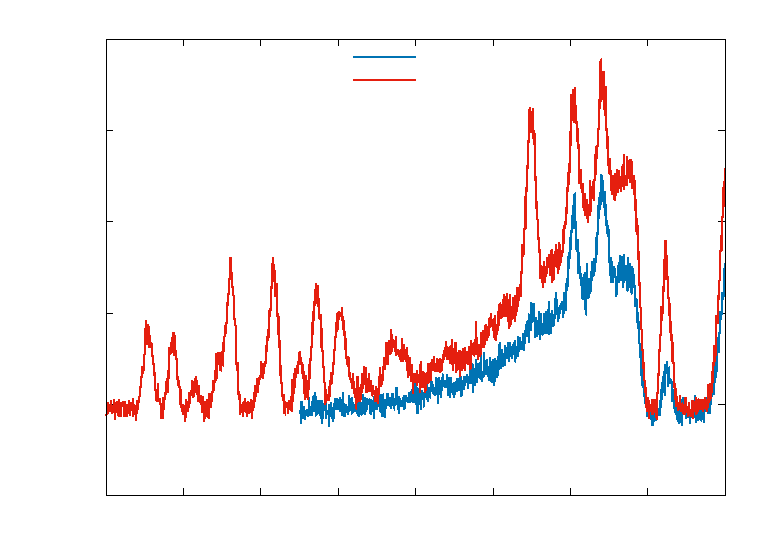
\includegraphics[width={360.00bp},height={252.00bp}]{Anhang/ccl4_s}}%
    \gplfronttext
  \end{picture}%
\endgroup
}}\\
    \subfigure[Anti-Stokes Linien]{\scalebox{0.9}{% GNUPLOT: LaTeX picture with Postscript
\begingroup
  % Encoding inside the plot.  In the header of your document, this encoding
  % should to defined, e.g., by using
  % \usepackage[cp1252,<other encodings>]{inputenc}
  \inputencoding{cp1252}%
  \makeatletter
  \providecommand\color[2][]{%
    \GenericError{(gnuplot) \space\space\space\@spaces}{%
      Package color not loaded in conjunction with
      terminal option `colourtext'%
    }{See the gnuplot documentation for explanation.%
    }{Either use 'blacktext' in gnuplot or load the package
      color.sty in LaTeX.}%
    \renewcommand\color[2][]{}%
  }%
  \providecommand\includegraphics[2][]{%
    \GenericError{(gnuplot) \space\space\space\@spaces}{%
      Package graphicx or graphics not loaded%
    }{See the gnuplot documentation for explanation.%
    }{The gnuplot epslatex terminal needs graphicx.sty or graphics.sty.}%
    \renewcommand\includegraphics[2][]{}%
  }%
  \providecommand\rotatebox[2]{#2}%
  \@ifundefined{ifGPcolor}{%
    \newif\ifGPcolor
    \GPcolorfalse
  }{}%
  \@ifundefined{ifGPblacktext}{%
    \newif\ifGPblacktext
    \GPblacktexttrue
  }{}%
  % define a \g@addto@macro without @ in the name:
  \let\gplgaddtomacro\g@addto@macro
  % define empty templates for all commands taking text:
  \gdef\gplbacktext{}%
  \gdef\gplfronttext{}%
  \makeatother
  \ifGPblacktext
    % no textcolor at all
    \def\colorrgb#1{}%
    \def\colorgray#1{}%
  \else
    % gray or color?
    \ifGPcolor
      \def\colorrgb#1{\color[rgb]{#1}}%
      \def\colorgray#1{\color[gray]{#1}}%
      \expandafter\def\csname LTw\endcsname{\color{white}}%
      \expandafter\def\csname LTb\endcsname{\color{black}}%
      \expandafter\def\csname LTa\endcsname{\color{black}}%
      \expandafter\def\csname LT0\endcsname{\color[rgb]{1,0,0}}%
      \expandafter\def\csname LT1\endcsname{\color[rgb]{0,1,0}}%
      \expandafter\def\csname LT2\endcsname{\color[rgb]{0,0,1}}%
      \expandafter\def\csname LT3\endcsname{\color[rgb]{1,0,1}}%
      \expandafter\def\csname LT4\endcsname{\color[rgb]{0,1,1}}%
      \expandafter\def\csname LT5\endcsname{\color[rgb]{1,1,0}}%
      \expandafter\def\csname LT6\endcsname{\color[rgb]{0,0,0}}%
      \expandafter\def\csname LT7\endcsname{\color[rgb]{1,0.3,0}}%
      \expandafter\def\csname LT8\endcsname{\color[rgb]{0.5,0.5,0.5}}%
    \else
      % gray
      \def\colorrgb#1{\color{black}}%
      \def\colorgray#1{\color[gray]{#1}}%
      \expandafter\def\csname LTw\endcsname{\color{white}}%
      \expandafter\def\csname LTb\endcsname{\color{black}}%
      \expandafter\def\csname LTa\endcsname{\color{black}}%
      \expandafter\def\csname LT0\endcsname{\color{black}}%
      \expandafter\def\csname LT1\endcsname{\color{black}}%
      \expandafter\def\csname LT2\endcsname{\color{black}}%
      \expandafter\def\csname LT3\endcsname{\color{black}}%
      \expandafter\def\csname LT4\endcsname{\color{black}}%
      \expandafter\def\csname LT5\endcsname{\color{black}}%
      \expandafter\def\csname LT6\endcsname{\color{black}}%
      \expandafter\def\csname LT7\endcsname{\color{black}}%
      \expandafter\def\csname LT8\endcsname{\color{black}}%
    \fi
  \fi
    \setlength{\unitlength}{0.0500bp}%
    \ifx\gptboxheight\undefined%
      \newlength{\gptboxheight}%
      \newlength{\gptboxwidth}%
      \newsavebox{\gptboxtext}%
    \fi%
    \setlength{\fboxrule}{0.5pt}%
    \setlength{\fboxsep}{1pt}%
\begin{picture}(7200.00,5040.00)%
    \gplgaddtomacro\gplbacktext{%
      \csname LTb\endcsname%%
      \put(594,440){\makebox(0,0)[r]{\strut{}$0$}}%
      \put(594,987){\makebox(0,0)[r]{\strut{}$0.1$}}%
      \put(594,1535){\makebox(0,0)[r]{\strut{}$0.2$}}%
      \put(594,2082){\makebox(0,0)[r]{\strut{}$0.3$}}%
      \put(594,2630){\makebox(0,0)[r]{\strut{}$0.4$}}%
      \put(594,3177){\makebox(0,0)[r]{\strut{}$0.5$}}%
      \put(594,3724){\makebox(0,0)[r]{\strut{}$0.6$}}%
      \put(594,4272){\makebox(0,0)[r]{\strut{}$0.7$}}%
      \put(594,4819){\makebox(0,0)[r]{\strut{}$0.8$}}%
      \put(726,220){\makebox(0,0){\strut{}$625$}}%
      \put(1334,220){\makebox(0,0){\strut{}$630$}}%
      \put(1941,220){\makebox(0,0){\strut{}$635$}}%
      \put(2549,220){\makebox(0,0){\strut{}$640$}}%
      \put(3157,220){\makebox(0,0){\strut{}$645$}}%
      \put(3765,220){\makebox(0,0){\strut{}$650$}}%
      \put(4372,220){\makebox(0,0){\strut{}$655$}}%
      \put(4980,220){\makebox(0,0){\strut{}$660$}}%
      \put(5588,220){\makebox(0,0){\strut{}$665$}}%
      \put(6195,220){\makebox(0,0){\strut{}$670$}}%
      \put(6803,220){\makebox(0,0){\strut{}$675$}}%
    }%
    \gplgaddtomacro\gplfronttext{%
      \csname LTb\endcsname%%
      \put(2970,4646){\makebox(0,0)[r]{\strut{}$0^\circ$ Polarisation}}%
      \csname LTb\endcsname%%
      \put(2970,4426){\makebox(0,0)[r]{\strut{}$90^\circ$ Polarisation}}%
    }%
    \gplbacktext
    \put(0,0){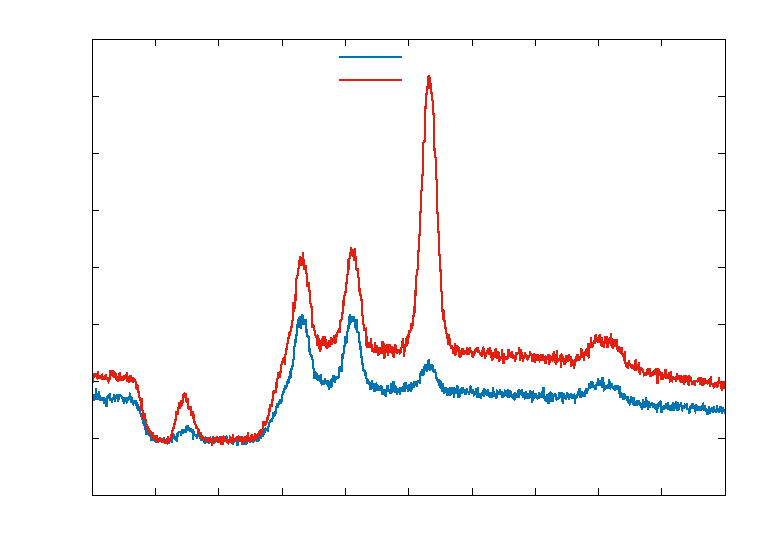
\includegraphics[width={360.00bp},height={252.00bp}]{Anhang/ccl4_as}}%
    \gplfronttext
  \end{picture}%
\endgroup
}}
    \caption{Gemessene Plots für Tetrachlormethan für $0^\circ$ und $90^\circ$-Polarisation im (Anti-)Stokes-Bereich}
\end{figure}\newpage
\section{Chlorophorm}
\begin{figure}[h]
    \centering\subfigure[Stokes Linien]{\scalebox{0.94}{% GNUPLOT: LaTeX picture with Postscript
\begingroup
  % Encoding inside the plot.  In the header of your document, this encoding
  % should to defined, e.g., by using
  % \usepackage[cp1252,<other encodings>]{inputenc}
  \inputencoding{cp1252}%
  \makeatletter
  \providecommand\color[2][]{%
    \GenericError{(gnuplot) \space\space\space\@spaces}{%
      Package color not loaded in conjunction with
      terminal option `colourtext'%
    }{See the gnuplot documentation for explanation.%
    }{Either use 'blacktext' in gnuplot or load the package
      color.sty in LaTeX.}%
    \renewcommand\color[2][]{}%
  }%
  \providecommand\includegraphics[2][]{%
    \GenericError{(gnuplot) \space\space\space\@spaces}{%
      Package graphicx or graphics not loaded%
    }{See the gnuplot documentation for explanation.%
    }{The gnuplot epslatex terminal needs graphicx.sty or graphics.sty.}%
    \renewcommand\includegraphics[2][]{}%
  }%
  \providecommand\rotatebox[2]{#2}%
  \@ifundefined{ifGPcolor}{%
    \newif\ifGPcolor
    \GPcolorfalse
  }{}%
  \@ifundefined{ifGPblacktext}{%
    \newif\ifGPblacktext
    \GPblacktexttrue
  }{}%
  % define a \g@addto@macro without @ in the name:
  \let\gplgaddtomacro\g@addto@macro
  % define empty templates for all commands taking text:
  \gdef\gplbacktext{}%
  \gdef\gplfronttext{}%
  \makeatother
  \ifGPblacktext
    % no textcolor at all
    \def\colorrgb#1{}%
    \def\colorgray#1{}%
  \else
    % gray or color?
    \ifGPcolor
      \def\colorrgb#1{\color[rgb]{#1}}%
      \def\colorgray#1{\color[gray]{#1}}%
      \expandafter\def\csname LTw\endcsname{\color{white}}%
      \expandafter\def\csname LTb\endcsname{\color{black}}%
      \expandafter\def\csname LTa\endcsname{\color{black}}%
      \expandafter\def\csname LT0\endcsname{\color[rgb]{1,0,0}}%
      \expandafter\def\csname LT1\endcsname{\color[rgb]{0,1,0}}%
      \expandafter\def\csname LT2\endcsname{\color[rgb]{0,0,1}}%
      \expandafter\def\csname LT3\endcsname{\color[rgb]{1,0,1}}%
      \expandafter\def\csname LT4\endcsname{\color[rgb]{0,1,1}}%
      \expandafter\def\csname LT5\endcsname{\color[rgb]{1,1,0}}%
      \expandafter\def\csname LT6\endcsname{\color[rgb]{0,0,0}}%
      \expandafter\def\csname LT7\endcsname{\color[rgb]{1,0.3,0}}%
      \expandafter\def\csname LT8\endcsname{\color[rgb]{0.5,0.5,0.5}}%
    \else
      % gray
      \def\colorrgb#1{\color{black}}%
      \def\colorgray#1{\color[gray]{#1}}%
      \expandafter\def\csname LTw\endcsname{\color{white}}%
      \expandafter\def\csname LTb\endcsname{\color{black}}%
      \expandafter\def\csname LTa\endcsname{\color{black}}%
      \expandafter\def\csname LT0\endcsname{\color{black}}%
      \expandafter\def\csname LT1\endcsname{\color{black}}%
      \expandafter\def\csname LT2\endcsname{\color{black}}%
      \expandafter\def\csname LT3\endcsname{\color{black}}%
      \expandafter\def\csname LT4\endcsname{\color{black}}%
      \expandafter\def\csname LT5\endcsname{\color{black}}%
      \expandafter\def\csname LT6\endcsname{\color{black}}%
      \expandafter\def\csname LT7\endcsname{\color{black}}%
      \expandafter\def\csname LT8\endcsname{\color{black}}%
    \fi
  \fi
    \setlength{\unitlength}{0.0500bp}%
    \ifx\gptboxheight\undefined%
      \newlength{\gptboxheight}%
      \newlength{\gptboxwidth}%
      \newsavebox{\gptboxtext}%
    \fi%
    \setlength{\fboxrule}{0.5pt}%
    \setlength{\fboxsep}{1pt}%
\begin{picture}(7200.00,5040.00)%
    \gplgaddtomacro\gplbacktext{%
      \csname LTb\endcsname%%
      \put(726,440){\makebox(0,0)[r]{\strut{}$0.08$}}%
      \put(726,1170){\makebox(0,0)[r]{\strut{}$0.1$}}%
      \put(726,1900){\makebox(0,0)[r]{\strut{}$0.12$}}%
      \put(726,2629){\makebox(0,0)[r]{\strut{}$0.14$}}%
      \put(726,3359){\makebox(0,0)[r]{\strut{}$0.16$}}%
      \put(726,4089){\makebox(0,0)[r]{\strut{}$0.18$}}%
      \put(726,4819){\makebox(0,0)[r]{\strut{}$0.2$}}%
      \put(858,220){\makebox(0,0){\strut{}$560$}}%
      \put(1601,220){\makebox(0,0){\strut{}$570$}}%
      \put(2344,220){\makebox(0,0){\strut{}$580$}}%
      \put(3087,220){\makebox(0,0){\strut{}$590$}}%
      \put(3831,220){\makebox(0,0){\strut{}$600$}}%
      \put(4574,220){\makebox(0,0){\strut{}$610$}}%
      \put(5317,220){\makebox(0,0){\strut{}$620$}}%
      \put(6060,220){\makebox(0,0){\strut{}$630$}}%
      \put(6803,220){\makebox(0,0){\strut{}$640$}}%
    }%
    \gplgaddtomacro\gplfronttext{%
      \csname LTb\endcsname%%
      \put(3102,4646){\makebox(0,0)[r]{\strut{}$0^\circ$ Polarisation}}%
      \csname LTb\endcsname%%
      \put(3102,4426){\makebox(0,0)[r]{\strut{}$90^\circ$ Polarisation}}%
    }%
    \gplbacktext
    \put(0,0){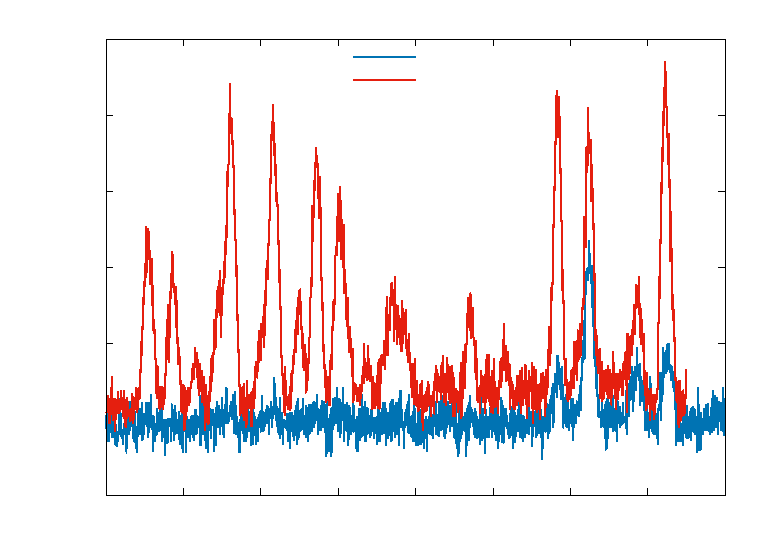
\includegraphics[width={360.00bp},height={252.00bp}]{Anhang/chcl3_s}}%
    \gplfronttext
  \end{picture}%
\endgroup
}}\\
    \subfigure[Anti-Stokes Linien]{\scalebox{0.94}{% GNUPLOT: LaTeX picture with Postscript
\begingroup
  % Encoding inside the plot.  In the header of your document, this encoding
  % should to defined, e.g., by using
  % \usepackage[cp1252,<other encodings>]{inputenc}
  \inputencoding{cp1252}%
  \makeatletter
  \providecommand\color[2][]{%
    \GenericError{(gnuplot) \space\space\space\@spaces}{%
      Package color not loaded in conjunction with
      terminal option `colourtext'%
    }{See the gnuplot documentation for explanation.%
    }{Either use 'blacktext' in gnuplot or load the package
      color.sty in LaTeX.}%
    \renewcommand\color[2][]{}%
  }%
  \providecommand\includegraphics[2][]{%
    \GenericError{(gnuplot) \space\space\space\@spaces}{%
      Package graphicx or graphics not loaded%
    }{See the gnuplot documentation for explanation.%
    }{The gnuplot epslatex terminal needs graphicx.sty or graphics.sty.}%
    \renewcommand\includegraphics[2][]{}%
  }%
  \providecommand\rotatebox[2]{#2}%
  \@ifundefined{ifGPcolor}{%
    \newif\ifGPcolor
    \GPcolorfalse
  }{}%
  \@ifundefined{ifGPblacktext}{%
    \newif\ifGPblacktext
    \GPblacktexttrue
  }{}%
  % define a \g@addto@macro without @ in the name:
  \let\gplgaddtomacro\g@addto@macro
  % define empty templates for all commands taking text:
  \gdef\gplbacktext{}%
  \gdef\gplfronttext{}%
  \makeatother
  \ifGPblacktext
    % no textcolor at all
    \def\colorrgb#1{}%
    \def\colorgray#1{}%
  \else
    % gray or color?
    \ifGPcolor
      \def\colorrgb#1{\color[rgb]{#1}}%
      \def\colorgray#1{\color[gray]{#1}}%
      \expandafter\def\csname LTw\endcsname{\color{white}}%
      \expandafter\def\csname LTb\endcsname{\color{black}}%
      \expandafter\def\csname LTa\endcsname{\color{black}}%
      \expandafter\def\csname LT0\endcsname{\color[rgb]{1,0,0}}%
      \expandafter\def\csname LT1\endcsname{\color[rgb]{0,1,0}}%
      \expandafter\def\csname LT2\endcsname{\color[rgb]{0,0,1}}%
      \expandafter\def\csname LT3\endcsname{\color[rgb]{1,0,1}}%
      \expandafter\def\csname LT4\endcsname{\color[rgb]{0,1,1}}%
      \expandafter\def\csname LT5\endcsname{\color[rgb]{1,1,0}}%
      \expandafter\def\csname LT6\endcsname{\color[rgb]{0,0,0}}%
      \expandafter\def\csname LT7\endcsname{\color[rgb]{1,0.3,0}}%
      \expandafter\def\csname LT8\endcsname{\color[rgb]{0.5,0.5,0.5}}%
    \else
      % gray
      \def\colorrgb#1{\color{black}}%
      \def\colorgray#1{\color[gray]{#1}}%
      \expandafter\def\csname LTw\endcsname{\color{white}}%
      \expandafter\def\csname LTb\endcsname{\color{black}}%
      \expandafter\def\csname LTa\endcsname{\color{black}}%
      \expandafter\def\csname LT0\endcsname{\color{black}}%
      \expandafter\def\csname LT1\endcsname{\color{black}}%
      \expandafter\def\csname LT2\endcsname{\color{black}}%
      \expandafter\def\csname LT3\endcsname{\color{black}}%
      \expandafter\def\csname LT4\endcsname{\color{black}}%
      \expandafter\def\csname LT5\endcsname{\color{black}}%
      \expandafter\def\csname LT6\endcsname{\color{black}}%
      \expandafter\def\csname LT7\endcsname{\color{black}}%
      \expandafter\def\csname LT8\endcsname{\color{black}}%
    \fi
  \fi
    \setlength{\unitlength}{0.0500bp}%
    \ifx\gptboxheight\undefined%
      \newlength{\gptboxheight}%
      \newlength{\gptboxwidth}%
      \newsavebox{\gptboxtext}%
    \fi%
    \setlength{\fboxrule}{0.5pt}%
    \setlength{\fboxsep}{1pt}%
\begin{picture}(7200.00,5040.00)%
    \gplgaddtomacro\gplbacktext{%
      \csname LTb\endcsname%%
      \put(726,440){\makebox(0,0)[r]{\strut{}$0.05$}}%
      \put(726,1066){\makebox(0,0)[r]{\strut{}$0.1$}}%
      \put(726,1691){\makebox(0,0)[r]{\strut{}$0.15$}}%
      \put(726,2317){\makebox(0,0)[r]{\strut{}$0.2$}}%
      \put(726,2942){\makebox(0,0)[r]{\strut{}$0.25$}}%
      \put(726,3568){\makebox(0,0)[r]{\strut{}$0.3$}}%
      \put(726,4193){\makebox(0,0)[r]{\strut{}$0.35$}}%
      \put(726,4819){\makebox(0,0)[r]{\strut{}$0.4$}}%
      \put(858,220){\makebox(0,0){\strut{}$620$}}%
      \put(1707,220){\makebox(0,0){\strut{}$630$}}%
      \put(2557,220){\makebox(0,0){\strut{}$640$}}%
      \put(3406,220){\makebox(0,0){\strut{}$650$}}%
      \put(4255,220){\makebox(0,0){\strut{}$660$}}%
      \put(5104,220){\makebox(0,0){\strut{}$670$}}%
      \put(5954,220){\makebox(0,0){\strut{}$680$}}%
      \put(6803,220){\makebox(0,0){\strut{}$690$}}%
    }%
    \gplgaddtomacro\gplfronttext{%
      \csname LTb\endcsname%%
      \put(3102,4646){\makebox(0,0)[r]{\strut{}$0^\circ$ Polarisation}}%
      \csname LTb\endcsname%%
      \put(3102,4426){\makebox(0,0)[r]{\strut{}$90^\circ$ Polarisation}}%
    }%
    \gplbacktext
    \put(0,0){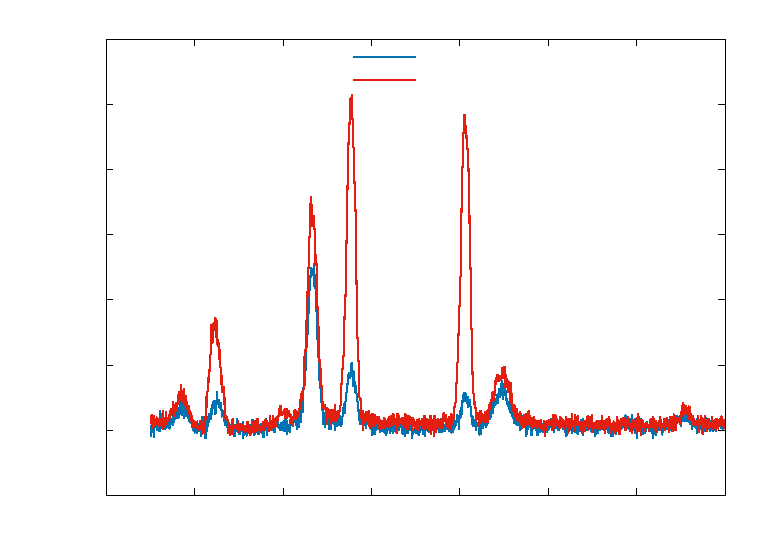
\includegraphics[width={360.00bp},height={252.00bp}]{Anhang/chcl3_as}}%
    \gplfronttext
  \end{picture}%
\endgroup
}}
    \caption{Gemessene Plots für Chlorophorm für $0^\circ$ und $90^\circ$-Polarisation im (Anti-)Stokes-Bereich}
\end{figure}\newpage
\section{Deuterium Chlorophorm}
\begin{figure}[h]
    \centering\subfigure[Stokes Linien]{\scalebox{0.94}{% GNUPLOT: LaTeX picture with Postscript
\begingroup
  % Encoding inside the plot.  In the header of your document, this encoding
  % should to defined, e.g., by using
  % \usepackage[cp1252,<other encodings>]{inputenc}
  \inputencoding{cp1252}%
  \makeatletter
  \providecommand\color[2][]{%
    \GenericError{(gnuplot) \space\space\space\@spaces}{%
      Package color not loaded in conjunction with
      terminal option `colourtext'%
    }{See the gnuplot documentation for explanation.%
    }{Either use 'blacktext' in gnuplot or load the package
      color.sty in LaTeX.}%
    \renewcommand\color[2][]{}%
  }%
  \providecommand\includegraphics[2][]{%
    \GenericError{(gnuplot) \space\space\space\@spaces}{%
      Package graphicx or graphics not loaded%
    }{See the gnuplot documentation for explanation.%
    }{The gnuplot epslatex terminal needs graphicx.sty or graphics.sty.}%
    \renewcommand\includegraphics[2][]{}%
  }%
  \providecommand\rotatebox[2]{#2}%
  \@ifundefined{ifGPcolor}{%
    \newif\ifGPcolor
    \GPcolorfalse
  }{}%
  \@ifundefined{ifGPblacktext}{%
    \newif\ifGPblacktext
    \GPblacktexttrue
  }{}%
  % define a \g@addto@macro without @ in the name:
  \let\gplgaddtomacro\g@addto@macro
  % define empty templates for all commands taking text:
  \gdef\gplbacktext{}%
  \gdef\gplfronttext{}%
  \makeatother
  \ifGPblacktext
    % no textcolor at all
    \def\colorrgb#1{}%
    \def\colorgray#1{}%
  \else
    % gray or color?
    \ifGPcolor
      \def\colorrgb#1{\color[rgb]{#1}}%
      \def\colorgray#1{\color[gray]{#1}}%
      \expandafter\def\csname LTw\endcsname{\color{white}}%
      \expandafter\def\csname LTb\endcsname{\color{black}}%
      \expandafter\def\csname LTa\endcsname{\color{black}}%
      \expandafter\def\csname LT0\endcsname{\color[rgb]{1,0,0}}%
      \expandafter\def\csname LT1\endcsname{\color[rgb]{0,1,0}}%
      \expandafter\def\csname LT2\endcsname{\color[rgb]{0,0,1}}%
      \expandafter\def\csname LT3\endcsname{\color[rgb]{1,0,1}}%
      \expandafter\def\csname LT4\endcsname{\color[rgb]{0,1,1}}%
      \expandafter\def\csname LT5\endcsname{\color[rgb]{1,1,0}}%
      \expandafter\def\csname LT6\endcsname{\color[rgb]{0,0,0}}%
      \expandafter\def\csname LT7\endcsname{\color[rgb]{1,0.3,0}}%
      \expandafter\def\csname LT8\endcsname{\color[rgb]{0.5,0.5,0.5}}%
    \else
      % gray
      \def\colorrgb#1{\color{black}}%
      \def\colorgray#1{\color[gray]{#1}}%
      \expandafter\def\csname LTw\endcsname{\color{white}}%
      \expandafter\def\csname LTb\endcsname{\color{black}}%
      \expandafter\def\csname LTa\endcsname{\color{black}}%
      \expandafter\def\csname LT0\endcsname{\color{black}}%
      \expandafter\def\csname LT1\endcsname{\color{black}}%
      \expandafter\def\csname LT2\endcsname{\color{black}}%
      \expandafter\def\csname LT3\endcsname{\color{black}}%
      \expandafter\def\csname LT4\endcsname{\color{black}}%
      \expandafter\def\csname LT5\endcsname{\color{black}}%
      \expandafter\def\csname LT6\endcsname{\color{black}}%
      \expandafter\def\csname LT7\endcsname{\color{black}}%
      \expandafter\def\csname LT8\endcsname{\color{black}}%
    \fi
  \fi
    \setlength{\unitlength}{0.0500bp}%
    \ifx\gptboxheight\undefined%
      \newlength{\gptboxheight}%
      \newlength{\gptboxwidth}%
      \newsavebox{\gptboxtext}%
    \fi%
    \setlength{\fboxrule}{0.5pt}%
    \setlength{\fboxsep}{1pt}%
\begin{picture}(7200.00,5040.00)%
    \gplgaddtomacro\gplbacktext{%
      \csname LTb\endcsname%%
      \put(726,440){\makebox(0,0)[r]{\strut{}$0.06$}}%
      \put(726,1066){\makebox(0,0)[r]{\strut{}$0.08$}}%
      \put(726,1691){\makebox(0,0)[r]{\strut{}$0.1$}}%
      \put(726,2317){\makebox(0,0)[r]{\strut{}$0.12$}}%
      \put(726,2942){\makebox(0,0)[r]{\strut{}$0.14$}}%
      \put(726,3568){\makebox(0,0)[r]{\strut{}$0.16$}}%
      \put(726,4193){\makebox(0,0)[r]{\strut{}$0.18$}}%
      \put(726,4819){\makebox(0,0)[r]{\strut{}$0.2$}}%
      \put(858,220){\makebox(0,0){\strut{}$570$}}%
      \put(1707,220){\makebox(0,0){\strut{}$580$}}%
      \put(2557,220){\makebox(0,0){\strut{}$590$}}%
      \put(3406,220){\makebox(0,0){\strut{}$600$}}%
      \put(4255,220){\makebox(0,0){\strut{}$610$}}%
      \put(5104,220){\makebox(0,0){\strut{}$620$}}%
      \put(5954,220){\makebox(0,0){\strut{}$630$}}%
      \put(6803,220){\makebox(0,0){\strut{}$640$}}%
    }%
    \gplgaddtomacro\gplfronttext{%
      \csname LTb\endcsname%%
      \put(3102,4646){\makebox(0,0)[r]{\strut{}$0^\circ$ Polarisation}}%
      \csname LTb\endcsname%%
      \put(3102,4426){\makebox(0,0)[r]{\strut{}$90^\circ$ Polarisation}}%
    }%
    \gplbacktext
    \put(0,0){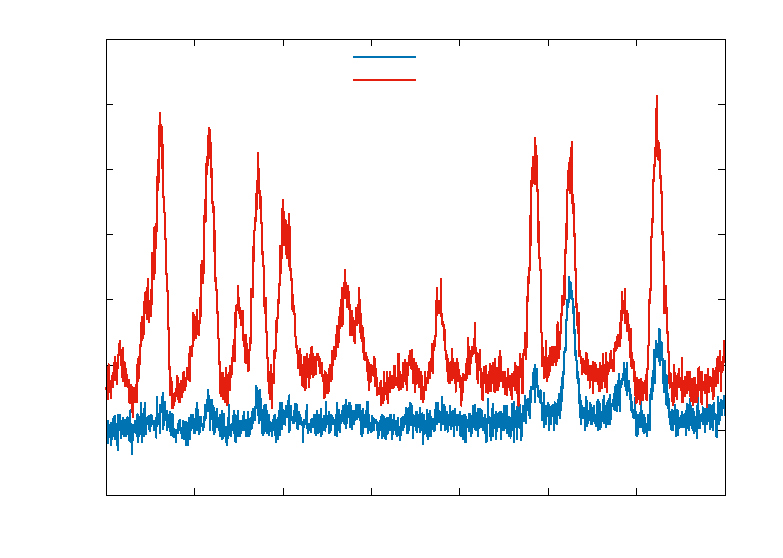
\includegraphics[width={360.00bp},height={252.00bp}]{Anhang/cdcl3_s}}%
    \gplfronttext
  \end{picture}%
\endgroup
}}\\
    \subfigure[Anti-Stokes Linien]{\scalebox{0.94}{% GNUPLOT: LaTeX picture with Postscript
\begingroup
  % Encoding inside the plot.  In the header of your document, this encoding
  % should to defined, e.g., by using
  % \usepackage[cp1252,<other encodings>]{inputenc}
  \inputencoding{cp1252}%
  \makeatletter
  \providecommand\color[2][]{%
    \GenericError{(gnuplot) \space\space\space\@spaces}{%
      Package color not loaded in conjunction with
      terminal option `colourtext'%
    }{See the gnuplot documentation for explanation.%
    }{Either use 'blacktext' in gnuplot or load the package
      color.sty in LaTeX.}%
    \renewcommand\color[2][]{}%
  }%
  \providecommand\includegraphics[2][]{%
    \GenericError{(gnuplot) \space\space\space\@spaces}{%
      Package graphicx or graphics not loaded%
    }{See the gnuplot documentation for explanation.%
    }{The gnuplot epslatex terminal needs graphicx.sty or graphics.sty.}%
    \renewcommand\includegraphics[2][]{}%
  }%
  \providecommand\rotatebox[2]{#2}%
  \@ifundefined{ifGPcolor}{%
    \newif\ifGPcolor
    \GPcolorfalse
  }{}%
  \@ifundefined{ifGPblacktext}{%
    \newif\ifGPblacktext
    \GPblacktexttrue
  }{}%
  % define a \g@addto@macro without @ in the name:
  \let\gplgaddtomacro\g@addto@macro
  % define empty templates for all commands taking text:
  \gdef\gplbacktext{}%
  \gdef\gplfronttext{}%
  \makeatother
  \ifGPblacktext
    % no textcolor at all
    \def\colorrgb#1{}%
    \def\colorgray#1{}%
  \else
    % gray or color?
    \ifGPcolor
      \def\colorrgb#1{\color[rgb]{#1}}%
      \def\colorgray#1{\color[gray]{#1}}%
      \expandafter\def\csname LTw\endcsname{\color{white}}%
      \expandafter\def\csname LTb\endcsname{\color{black}}%
      \expandafter\def\csname LTa\endcsname{\color{black}}%
      \expandafter\def\csname LT0\endcsname{\color[rgb]{1,0,0}}%
      \expandafter\def\csname LT1\endcsname{\color[rgb]{0,1,0}}%
      \expandafter\def\csname LT2\endcsname{\color[rgb]{0,0,1}}%
      \expandafter\def\csname LT3\endcsname{\color[rgb]{1,0,1}}%
      \expandafter\def\csname LT4\endcsname{\color[rgb]{0,1,1}}%
      \expandafter\def\csname LT5\endcsname{\color[rgb]{1,1,0}}%
      \expandafter\def\csname LT6\endcsname{\color[rgb]{0,0,0}}%
      \expandafter\def\csname LT7\endcsname{\color[rgb]{1,0.3,0}}%
      \expandafter\def\csname LT8\endcsname{\color[rgb]{0.5,0.5,0.5}}%
    \else
      % gray
      \def\colorrgb#1{\color{black}}%
      \def\colorgray#1{\color[gray]{#1}}%
      \expandafter\def\csname LTw\endcsname{\color{white}}%
      \expandafter\def\csname LTb\endcsname{\color{black}}%
      \expandafter\def\csname LTa\endcsname{\color{black}}%
      \expandafter\def\csname LT0\endcsname{\color{black}}%
      \expandafter\def\csname LT1\endcsname{\color{black}}%
      \expandafter\def\csname LT2\endcsname{\color{black}}%
      \expandafter\def\csname LT3\endcsname{\color{black}}%
      \expandafter\def\csname LT4\endcsname{\color{black}}%
      \expandafter\def\csname LT5\endcsname{\color{black}}%
      \expandafter\def\csname LT6\endcsname{\color{black}}%
      \expandafter\def\csname LT7\endcsname{\color{black}}%
      \expandafter\def\csname LT8\endcsname{\color{black}}%
    \fi
  \fi
    \setlength{\unitlength}{0.0500bp}%
    \ifx\gptboxheight\undefined%
      \newlength{\gptboxheight}%
      \newlength{\gptboxwidth}%
      \newsavebox{\gptboxtext}%
    \fi%
    \setlength{\fboxrule}{0.5pt}%
    \setlength{\fboxsep}{1pt}%
\begin{picture}(7200.00,5040.00)%
    \gplgaddtomacro\gplbacktext{%
      \csname LTb\endcsname%%
      \put(726,440){\makebox(0,0)[r]{\strut{}$0.05$}}%
      \put(726,1066){\makebox(0,0)[r]{\strut{}$0.1$}}%
      \put(726,1691){\makebox(0,0)[r]{\strut{}$0.15$}}%
      \put(726,2317){\makebox(0,0)[r]{\strut{}$0.2$}}%
      \put(726,2942){\makebox(0,0)[r]{\strut{}$0.25$}}%
      \put(726,3568){\makebox(0,0)[r]{\strut{}$0.3$}}%
      \put(726,4193){\makebox(0,0)[r]{\strut{}$0.35$}}%
      \put(726,4819){\makebox(0,0)[r]{\strut{}$0.4$}}%
      \put(858,220){\makebox(0,0){\strut{}$620$}}%
      \put(1601,220){\makebox(0,0){\strut{}$630$}}%
      \put(2344,220){\makebox(0,0){\strut{}$640$}}%
      \put(3087,220){\makebox(0,0){\strut{}$650$}}%
      \put(3831,220){\makebox(0,0){\strut{}$660$}}%
      \put(4574,220){\makebox(0,0){\strut{}$670$}}%
      \put(5317,220){\makebox(0,0){\strut{}$680$}}%
      \put(6060,220){\makebox(0,0){\strut{}$690$}}%
      \put(6803,220){\makebox(0,0){\strut{}$700$}}%
    }%
    \gplgaddtomacro\gplfronttext{%
      \csname LTb\endcsname%%
      \put(3102,4646){\makebox(0,0)[r]{\strut{}$0^\circ$ Polarisation}}%
      \csname LTb\endcsname%%
      \put(3102,4426){\makebox(0,0)[r]{\strut{}$90^\circ$ Polarisation}}%
    }%
    \gplbacktext
    \put(0,0){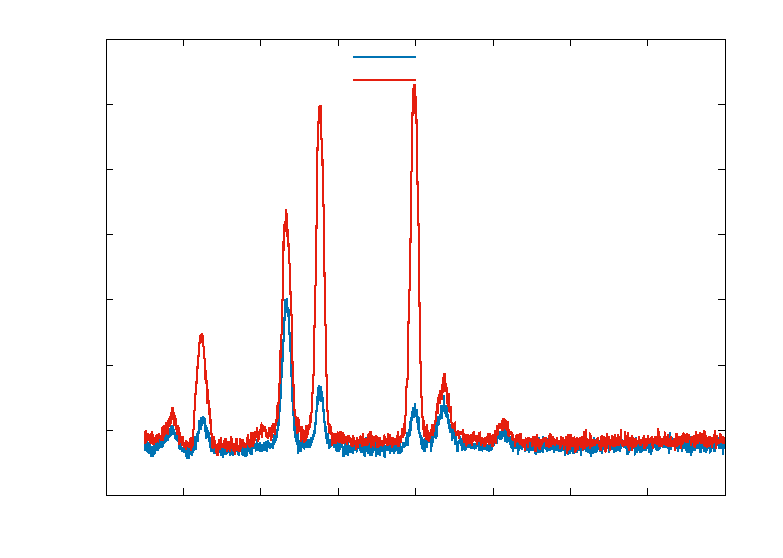
\includegraphics[width={360.00bp},height={252.00bp}]{Anhang/cdcl3_as}}%
    \gplfronttext
  \end{picture}%
\endgroup
}}
    \caption{Gemessene Plots für Deuterium Chlorophorm für $0^\circ$ und $90^\circ$-Polarisation im (Anti-)Stokes-Bereich}
\end{figure}\newpage
\section{Bromophorm}
\begin{figure}[h]
    \centering\subfigure[Stokes Linien]{\scalebox{0.94}{% GNUPLOT: LaTeX picture with Postscript
\begingroup
  % Encoding inside the plot.  In the header of your document, this encoding
  % should to defined, e.g., by using
  % \usepackage[cp1252,<other encodings>]{inputenc}
  \inputencoding{cp1252}%
  \makeatletter
  \providecommand\color[2][]{%
    \GenericError{(gnuplot) \space\space\space\@spaces}{%
      Package color not loaded in conjunction with
      terminal option `colourtext'%
    }{See the gnuplot documentation for explanation.%
    }{Either use 'blacktext' in gnuplot or load the package
      color.sty in LaTeX.}%
    \renewcommand\color[2][]{}%
  }%
  \providecommand\includegraphics[2][]{%
    \GenericError{(gnuplot) \space\space\space\@spaces}{%
      Package graphicx or graphics not loaded%
    }{See the gnuplot documentation for explanation.%
    }{The gnuplot epslatex terminal needs graphicx.sty or graphics.sty.}%
    \renewcommand\includegraphics[2][]{}%
  }%
  \providecommand\rotatebox[2]{#2}%
  \@ifundefined{ifGPcolor}{%
    \newif\ifGPcolor
    \GPcolorfalse
  }{}%
  \@ifundefined{ifGPblacktext}{%
    \newif\ifGPblacktext
    \GPblacktexttrue
  }{}%
  % define a \g@addto@macro without @ in the name:
  \let\gplgaddtomacro\g@addto@macro
  % define empty templates for all commands taking text:
  \gdef\gplbacktext{}%
  \gdef\gplfronttext{}%
  \makeatother
  \ifGPblacktext
    % no textcolor at all
    \def\colorrgb#1{}%
    \def\colorgray#1{}%
  \else
    % gray or color?
    \ifGPcolor
      \def\colorrgb#1{\color[rgb]{#1}}%
      \def\colorgray#1{\color[gray]{#1}}%
      \expandafter\def\csname LTw\endcsname{\color{white}}%
      \expandafter\def\csname LTb\endcsname{\color{black}}%
      \expandafter\def\csname LTa\endcsname{\color{black}}%
      \expandafter\def\csname LT0\endcsname{\color[rgb]{1,0,0}}%
      \expandafter\def\csname LT1\endcsname{\color[rgb]{0,1,0}}%
      \expandafter\def\csname LT2\endcsname{\color[rgb]{0,0,1}}%
      \expandafter\def\csname LT3\endcsname{\color[rgb]{1,0,1}}%
      \expandafter\def\csname LT4\endcsname{\color[rgb]{0,1,1}}%
      \expandafter\def\csname LT5\endcsname{\color[rgb]{1,1,0}}%
      \expandafter\def\csname LT6\endcsname{\color[rgb]{0,0,0}}%
      \expandafter\def\csname LT7\endcsname{\color[rgb]{1,0.3,0}}%
      \expandafter\def\csname LT8\endcsname{\color[rgb]{0.5,0.5,0.5}}%
    \else
      % gray
      \def\colorrgb#1{\color{black}}%
      \def\colorgray#1{\color[gray]{#1}}%
      \expandafter\def\csname LTw\endcsname{\color{white}}%
      \expandafter\def\csname LTb\endcsname{\color{black}}%
      \expandafter\def\csname LTa\endcsname{\color{black}}%
      \expandafter\def\csname LT0\endcsname{\color{black}}%
      \expandafter\def\csname LT1\endcsname{\color{black}}%
      \expandafter\def\csname LT2\endcsname{\color{black}}%
      \expandafter\def\csname LT3\endcsname{\color{black}}%
      \expandafter\def\csname LT4\endcsname{\color{black}}%
      \expandafter\def\csname LT5\endcsname{\color{black}}%
      \expandafter\def\csname LT6\endcsname{\color{black}}%
      \expandafter\def\csname LT7\endcsname{\color{black}}%
      \expandafter\def\csname LT8\endcsname{\color{black}}%
    \fi
  \fi
    \setlength{\unitlength}{0.0500bp}%
    \ifx\gptboxheight\undefined%
      \newlength{\gptboxheight}%
      \newlength{\gptboxwidth}%
      \newsavebox{\gptboxtext}%
    \fi%
    \setlength{\fboxrule}{0.5pt}%
    \setlength{\fboxsep}{1pt}%
\begin{picture}(7200.00,5040.00)%
    \gplgaddtomacro\gplbacktext{%
      \csname LTb\endcsname%%
      \put(726,440){\makebox(0,0)[r]{\strut{}$0.05$}}%
      \put(726,927){\makebox(0,0)[r]{\strut{}$0.1$}}%
      \put(726,1413){\makebox(0,0)[r]{\strut{}$0.15$}}%
      \put(726,1900){\makebox(0,0)[r]{\strut{}$0.2$}}%
      \put(726,2386){\makebox(0,0)[r]{\strut{}$0.25$}}%
      \put(726,2873){\makebox(0,0)[r]{\strut{}$0.3$}}%
      \put(726,3359){\makebox(0,0)[r]{\strut{}$0.35$}}%
      \put(726,3846){\makebox(0,0)[r]{\strut{}$0.4$}}%
      \put(726,4332){\makebox(0,0)[r]{\strut{}$0.45$}}%
      \put(726,4819){\makebox(0,0)[r]{\strut{}$0.5$}}%
      \put(858,220){\makebox(0,0){\strut{}$560$}}%
      \put(1601,220){\makebox(0,0){\strut{}$570$}}%
      \put(2344,220){\makebox(0,0){\strut{}$580$}}%
      \put(3087,220){\makebox(0,0){\strut{}$590$}}%
      \put(3831,220){\makebox(0,0){\strut{}$600$}}%
      \put(4574,220){\makebox(0,0){\strut{}$610$}}%
      \put(5317,220){\makebox(0,0){\strut{}$620$}}%
      \put(6060,220){\makebox(0,0){\strut{}$630$}}%
      \put(6803,220){\makebox(0,0){\strut{}$640$}}%
    }%
    \gplgaddtomacro\gplfronttext{%
      \csname LTb\endcsname%%
      \put(3102,4646){\makebox(0,0)[r]{\strut{}$0^\circ$ Polarisation}}%
      \csname LTb\endcsname%%
      \put(3102,4426){\makebox(0,0)[r]{\strut{}$90^\circ$ Polarisation}}%
    }%
    \gplbacktext
    \put(0,0){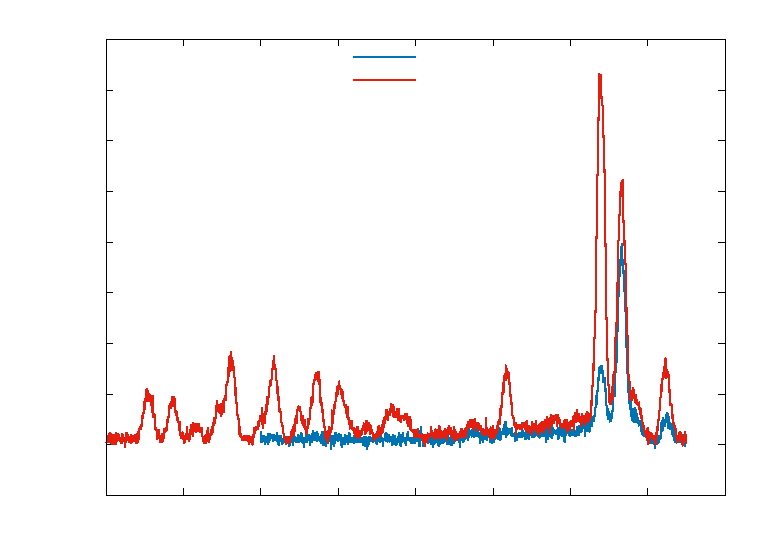
\includegraphics[width={360.00bp},height={252.00bp}]{Anhang/chbr3_s}}%
    \gplfronttext
  \end{picture}%
\endgroup
}}\\
    \subfigure[Anti-Stokes Linien]{\scalebox{0.94}{% GNUPLOT: LaTeX picture with Postscript
\begingroup
  % Encoding inside the plot.  In the header of your document, this encoding
  % should to defined, e.g., by using
  % \usepackage[cp1252,<other encodings>]{inputenc}
  \inputencoding{cp1252}%
  \makeatletter
  \providecommand\color[2][]{%
    \GenericError{(gnuplot) \space\space\space\@spaces}{%
      Package color not loaded in conjunction with
      terminal option `colourtext'%
    }{See the gnuplot documentation for explanation.%
    }{Either use 'blacktext' in gnuplot or load the package
      color.sty in LaTeX.}%
    \renewcommand\color[2][]{}%
  }%
  \providecommand\includegraphics[2][]{%
    \GenericError{(gnuplot) \space\space\space\@spaces}{%
      Package graphicx or graphics not loaded%
    }{See the gnuplot documentation for explanation.%
    }{The gnuplot epslatex terminal needs graphicx.sty or graphics.sty.}%
    \renewcommand\includegraphics[2][]{}%
  }%
  \providecommand\rotatebox[2]{#2}%
  \@ifundefined{ifGPcolor}{%
    \newif\ifGPcolor
    \GPcolorfalse
  }{}%
  \@ifundefined{ifGPblacktext}{%
    \newif\ifGPblacktext
    \GPblacktexttrue
  }{}%
  % define a \g@addto@macro without @ in the name:
  \let\gplgaddtomacro\g@addto@macro
  % define empty templates for all commands taking text:
  \gdef\gplbacktext{}%
  \gdef\gplfronttext{}%
  \makeatother
  \ifGPblacktext
    % no textcolor at all
    \def\colorrgb#1{}%
    \def\colorgray#1{}%
  \else
    % gray or color?
    \ifGPcolor
      \def\colorrgb#1{\color[rgb]{#1}}%
      \def\colorgray#1{\color[gray]{#1}}%
      \expandafter\def\csname LTw\endcsname{\color{white}}%
      \expandafter\def\csname LTb\endcsname{\color{black}}%
      \expandafter\def\csname LTa\endcsname{\color{black}}%
      \expandafter\def\csname LT0\endcsname{\color[rgb]{1,0,0}}%
      \expandafter\def\csname LT1\endcsname{\color[rgb]{0,1,0}}%
      \expandafter\def\csname LT2\endcsname{\color[rgb]{0,0,1}}%
      \expandafter\def\csname LT3\endcsname{\color[rgb]{1,0,1}}%
      \expandafter\def\csname LT4\endcsname{\color[rgb]{0,1,1}}%
      \expandafter\def\csname LT5\endcsname{\color[rgb]{1,1,0}}%
      \expandafter\def\csname LT6\endcsname{\color[rgb]{0,0,0}}%
      \expandafter\def\csname LT7\endcsname{\color[rgb]{1,0.3,0}}%
      \expandafter\def\csname LT8\endcsname{\color[rgb]{0.5,0.5,0.5}}%
    \else
      % gray
      \def\colorrgb#1{\color{black}}%
      \def\colorgray#1{\color[gray]{#1}}%
      \expandafter\def\csname LTw\endcsname{\color{white}}%
      \expandafter\def\csname LTb\endcsname{\color{black}}%
      \expandafter\def\csname LTa\endcsname{\color{black}}%
      \expandafter\def\csname LT0\endcsname{\color{black}}%
      \expandafter\def\csname LT1\endcsname{\color{black}}%
      \expandafter\def\csname LT2\endcsname{\color{black}}%
      \expandafter\def\csname LT3\endcsname{\color{black}}%
      \expandafter\def\csname LT4\endcsname{\color{black}}%
      \expandafter\def\csname LT5\endcsname{\color{black}}%
      \expandafter\def\csname LT6\endcsname{\color{black}}%
      \expandafter\def\csname LT7\endcsname{\color{black}}%
      \expandafter\def\csname LT8\endcsname{\color{black}}%
    \fi
  \fi
    \setlength{\unitlength}{0.0500bp}%
    \ifx\gptboxheight\undefined%
      \newlength{\gptboxheight}%
      \newlength{\gptboxwidth}%
      \newsavebox{\gptboxtext}%
    \fi%
    \setlength{\fboxrule}{0.5pt}%
    \setlength{\fboxsep}{1pt}%
\begin{picture}(7200.00,5040.00)%
    \gplgaddtomacro\gplbacktext{%
      \csname LTb\endcsname%%
      \put(594,440){\makebox(0,0)[r]{\strut{}$0$}}%
      \put(594,927){\makebox(0,0)[r]{\strut{}$0.1$}}%
      \put(594,1413){\makebox(0,0)[r]{\strut{}$0.2$}}%
      \put(594,1900){\makebox(0,0)[r]{\strut{}$0.3$}}%
      \put(594,2386){\makebox(0,0)[r]{\strut{}$0.4$}}%
      \put(594,2873){\makebox(0,0)[r]{\strut{}$0.5$}}%
      \put(594,3359){\makebox(0,0)[r]{\strut{}$0.6$}}%
      \put(594,3846){\makebox(0,0)[r]{\strut{}$0.7$}}%
      \put(594,4332){\makebox(0,0)[r]{\strut{}$0.8$}}%
      \put(594,4819){\makebox(0,0)[r]{\strut{}$0.9$}}%
      \put(726,220){\makebox(0,0){\strut{}$620$}}%
      \put(1594,220){\makebox(0,0){\strut{}$630$}}%
      \put(2462,220){\makebox(0,0){\strut{}$640$}}%
      \put(3330,220){\makebox(0,0){\strut{}$650$}}%
      \put(4199,220){\makebox(0,0){\strut{}$660$}}%
      \put(5067,220){\makebox(0,0){\strut{}$670$}}%
      \put(5935,220){\makebox(0,0){\strut{}$680$}}%
      \put(6803,220){\makebox(0,0){\strut{}$690$}}%
    }%
    \gplgaddtomacro\gplfronttext{%
      \csname LTb\endcsname%%
      \put(5816,4646){\makebox(0,0)[r]{\strut{}$0^\circ$ Polarisation}}%
      \csname LTb\endcsname%%
      \put(5816,4426){\makebox(0,0)[r]{\strut{}$90^\circ$ Polarisation}}%
    }%
    \gplbacktext
    \put(0,0){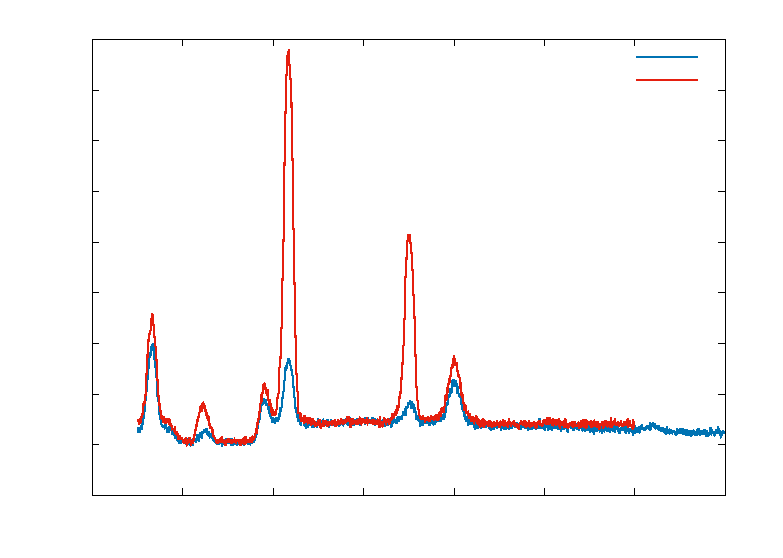
\includegraphics[width={360.00bp},height={252.00bp}]{Anhang/chbr3_as}}%
    \gplfronttext
  \end{picture}%
\endgroup
}}
    \caption{Gemessene Plots für Bromophorm für $0^\circ$ und $90^\circ$-Polarisation im (Anti-)Stokes-Bereich}
\end{figure}\newpage
\chapter{Gemessene Plots}
\section{Tetrachlormethan}
\begin{figure}[h]
    \centering\subfigure[Stokes Linien]{\scalebox{0.9}{% GNUPLOT: LaTeX picture with Postscript
\begingroup
  % Encoding inside the plot.  In the header of your document, this encoding
  % should to defined, e.g., by using
  % \usepackage[cp1252,<other encodings>]{inputenc}
  \inputencoding{cp1252}%
  \makeatletter
  \providecommand\color[2][]{%
    \GenericError{(gnuplot) \space\space\space\@spaces}{%
      Package color not loaded in conjunction with
      terminal option `colourtext'%
    }{See the gnuplot documentation for explanation.%
    }{Either use 'blacktext' in gnuplot or load the package
      color.sty in LaTeX.}%
    \renewcommand\color[2][]{}%
  }%
  \providecommand\includegraphics[2][]{%
    \GenericError{(gnuplot) \space\space\space\@spaces}{%
      Package graphicx or graphics not loaded%
    }{See the gnuplot documentation for explanation.%
    }{The gnuplot epslatex terminal needs graphicx.sty or graphics.sty.}%
    \renewcommand\includegraphics[2][]{}%
  }%
  \providecommand\rotatebox[2]{#2}%
  \@ifundefined{ifGPcolor}{%
    \newif\ifGPcolor
    \GPcolorfalse
  }{}%
  \@ifundefined{ifGPblacktext}{%
    \newif\ifGPblacktext
    \GPblacktexttrue
  }{}%
  % define a \g@addto@macro without @ in the name:
  \let\gplgaddtomacro\g@addto@macro
  % define empty templates for all commands taking text:
  \gdef\gplbacktext{}%
  \gdef\gplfronttext{}%
  \makeatother
  \ifGPblacktext
    % no textcolor at all
    \def\colorrgb#1{}%
    \def\colorgray#1{}%
  \else
    % gray or color?
    \ifGPcolor
      \def\colorrgb#1{\color[rgb]{#1}}%
      \def\colorgray#1{\color[gray]{#1}}%
      \expandafter\def\csname LTw\endcsname{\color{white}}%
      \expandafter\def\csname LTb\endcsname{\color{black}}%
      \expandafter\def\csname LTa\endcsname{\color{black}}%
      \expandafter\def\csname LT0\endcsname{\color[rgb]{1,0,0}}%
      \expandafter\def\csname LT1\endcsname{\color[rgb]{0,1,0}}%
      \expandafter\def\csname LT2\endcsname{\color[rgb]{0,0,1}}%
      \expandafter\def\csname LT3\endcsname{\color[rgb]{1,0,1}}%
      \expandafter\def\csname LT4\endcsname{\color[rgb]{0,1,1}}%
      \expandafter\def\csname LT5\endcsname{\color[rgb]{1,1,0}}%
      \expandafter\def\csname LT6\endcsname{\color[rgb]{0,0,0}}%
      \expandafter\def\csname LT7\endcsname{\color[rgb]{1,0.3,0}}%
      \expandafter\def\csname LT8\endcsname{\color[rgb]{0.5,0.5,0.5}}%
    \else
      % gray
      \def\colorrgb#1{\color{black}}%
      \def\colorgray#1{\color[gray]{#1}}%
      \expandafter\def\csname LTw\endcsname{\color{white}}%
      \expandafter\def\csname LTb\endcsname{\color{black}}%
      \expandafter\def\csname LTa\endcsname{\color{black}}%
      \expandafter\def\csname LT0\endcsname{\color{black}}%
      \expandafter\def\csname LT1\endcsname{\color{black}}%
      \expandafter\def\csname LT2\endcsname{\color{black}}%
      \expandafter\def\csname LT3\endcsname{\color{black}}%
      \expandafter\def\csname LT4\endcsname{\color{black}}%
      \expandafter\def\csname LT5\endcsname{\color{black}}%
      \expandafter\def\csname LT6\endcsname{\color{black}}%
      \expandafter\def\csname LT7\endcsname{\color{black}}%
      \expandafter\def\csname LT8\endcsname{\color{black}}%
    \fi
  \fi
    \setlength{\unitlength}{0.0500bp}%
    \ifx\gptboxheight\undefined%
      \newlength{\gptboxheight}%
      \newlength{\gptboxwidth}%
      \newsavebox{\gptboxtext}%
    \fi%
    \setlength{\fboxrule}{0.5pt}%
    \setlength{\fboxsep}{1pt}%
\begin{picture}(7200.00,5040.00)%
    \gplgaddtomacro\gplbacktext{%
      \csname LTb\endcsname%%
      \put(726,440){\makebox(0,0)[r]{\strut{}$0.05$}}%
      \put(726,1316){\makebox(0,0)[r]{\strut{}$0.1$}}%
      \put(726,2192){\makebox(0,0)[r]{\strut{}$0.15$}}%
      \put(726,3067){\makebox(0,0)[r]{\strut{}$0.2$}}%
      \put(726,3943){\makebox(0,0)[r]{\strut{}$0.25$}}%
      \put(726,4819){\makebox(0,0)[r]{\strut{}$0.3$}}%
      \put(858,220){\makebox(0,0){\strut{}$560$}}%
      \put(1601,220){\makebox(0,0){\strut{}$570$}}%
      \put(2344,220){\makebox(0,0){\strut{}$580$}}%
      \put(3087,220){\makebox(0,0){\strut{}$590$}}%
      \put(3831,220){\makebox(0,0){\strut{}$600$}}%
      \put(4574,220){\makebox(0,0){\strut{}$610$}}%
      \put(5317,220){\makebox(0,0){\strut{}$620$}}%
      \put(6060,220){\makebox(0,0){\strut{}$630$}}%
      \put(6803,220){\makebox(0,0){\strut{}$640$}}%
    }%
    \gplgaddtomacro\gplfronttext{%
      \csname LTb\endcsname%%
      \put(3102,4646){\makebox(0,0)[r]{\strut{}$0^\circ$ Polarisation}}%
      \csname LTb\endcsname%%
      \put(3102,4426){\makebox(0,0)[r]{\strut{}$90^\circ$ Polarisation}}%
    }%
    \gplbacktext
    \put(0,0){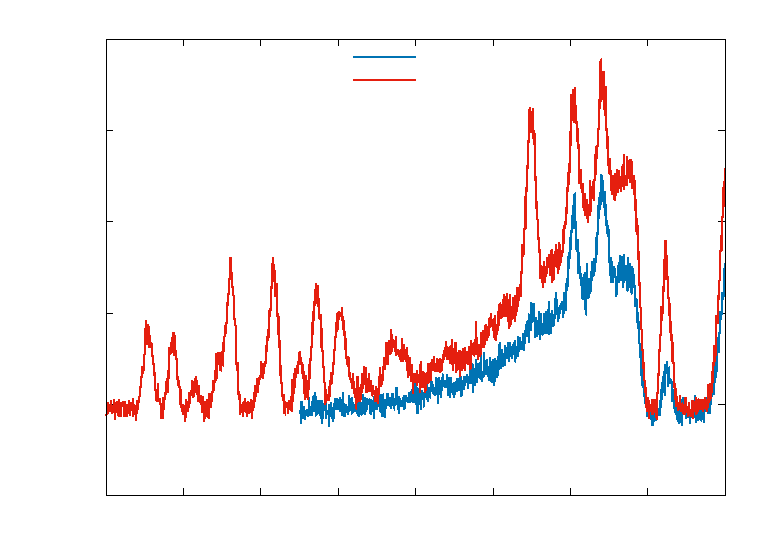
\includegraphics[width={360.00bp},height={252.00bp}]{Anhang/ccl4_s}}%
    \gplfronttext
  \end{picture}%
\endgroup
}}\\
    \subfigure[Anti-Stokes Linien]{\scalebox{0.9}{% GNUPLOT: LaTeX picture with Postscript
\begingroup
  % Encoding inside the plot.  In the header of your document, this encoding
  % should to defined, e.g., by using
  % \usepackage[cp1252,<other encodings>]{inputenc}
  \inputencoding{cp1252}%
  \makeatletter
  \providecommand\color[2][]{%
    \GenericError{(gnuplot) \space\space\space\@spaces}{%
      Package color not loaded in conjunction with
      terminal option `colourtext'%
    }{See the gnuplot documentation for explanation.%
    }{Either use 'blacktext' in gnuplot or load the package
      color.sty in LaTeX.}%
    \renewcommand\color[2][]{}%
  }%
  \providecommand\includegraphics[2][]{%
    \GenericError{(gnuplot) \space\space\space\@spaces}{%
      Package graphicx or graphics not loaded%
    }{See the gnuplot documentation for explanation.%
    }{The gnuplot epslatex terminal needs graphicx.sty or graphics.sty.}%
    \renewcommand\includegraphics[2][]{}%
  }%
  \providecommand\rotatebox[2]{#2}%
  \@ifundefined{ifGPcolor}{%
    \newif\ifGPcolor
    \GPcolorfalse
  }{}%
  \@ifundefined{ifGPblacktext}{%
    \newif\ifGPblacktext
    \GPblacktexttrue
  }{}%
  % define a \g@addto@macro without @ in the name:
  \let\gplgaddtomacro\g@addto@macro
  % define empty templates for all commands taking text:
  \gdef\gplbacktext{}%
  \gdef\gplfronttext{}%
  \makeatother
  \ifGPblacktext
    % no textcolor at all
    \def\colorrgb#1{}%
    \def\colorgray#1{}%
  \else
    % gray or color?
    \ifGPcolor
      \def\colorrgb#1{\color[rgb]{#1}}%
      \def\colorgray#1{\color[gray]{#1}}%
      \expandafter\def\csname LTw\endcsname{\color{white}}%
      \expandafter\def\csname LTb\endcsname{\color{black}}%
      \expandafter\def\csname LTa\endcsname{\color{black}}%
      \expandafter\def\csname LT0\endcsname{\color[rgb]{1,0,0}}%
      \expandafter\def\csname LT1\endcsname{\color[rgb]{0,1,0}}%
      \expandafter\def\csname LT2\endcsname{\color[rgb]{0,0,1}}%
      \expandafter\def\csname LT3\endcsname{\color[rgb]{1,0,1}}%
      \expandafter\def\csname LT4\endcsname{\color[rgb]{0,1,1}}%
      \expandafter\def\csname LT5\endcsname{\color[rgb]{1,1,0}}%
      \expandafter\def\csname LT6\endcsname{\color[rgb]{0,0,0}}%
      \expandafter\def\csname LT7\endcsname{\color[rgb]{1,0.3,0}}%
      \expandafter\def\csname LT8\endcsname{\color[rgb]{0.5,0.5,0.5}}%
    \else
      % gray
      \def\colorrgb#1{\color{black}}%
      \def\colorgray#1{\color[gray]{#1}}%
      \expandafter\def\csname LTw\endcsname{\color{white}}%
      \expandafter\def\csname LTb\endcsname{\color{black}}%
      \expandafter\def\csname LTa\endcsname{\color{black}}%
      \expandafter\def\csname LT0\endcsname{\color{black}}%
      \expandafter\def\csname LT1\endcsname{\color{black}}%
      \expandafter\def\csname LT2\endcsname{\color{black}}%
      \expandafter\def\csname LT3\endcsname{\color{black}}%
      \expandafter\def\csname LT4\endcsname{\color{black}}%
      \expandafter\def\csname LT5\endcsname{\color{black}}%
      \expandafter\def\csname LT6\endcsname{\color{black}}%
      \expandafter\def\csname LT7\endcsname{\color{black}}%
      \expandafter\def\csname LT8\endcsname{\color{black}}%
    \fi
  \fi
    \setlength{\unitlength}{0.0500bp}%
    \ifx\gptboxheight\undefined%
      \newlength{\gptboxheight}%
      \newlength{\gptboxwidth}%
      \newsavebox{\gptboxtext}%
    \fi%
    \setlength{\fboxrule}{0.5pt}%
    \setlength{\fboxsep}{1pt}%
\begin{picture}(7200.00,5040.00)%
    \gplgaddtomacro\gplbacktext{%
      \csname LTb\endcsname%%
      \put(594,440){\makebox(0,0)[r]{\strut{}$0$}}%
      \put(594,987){\makebox(0,0)[r]{\strut{}$0.1$}}%
      \put(594,1535){\makebox(0,0)[r]{\strut{}$0.2$}}%
      \put(594,2082){\makebox(0,0)[r]{\strut{}$0.3$}}%
      \put(594,2630){\makebox(0,0)[r]{\strut{}$0.4$}}%
      \put(594,3177){\makebox(0,0)[r]{\strut{}$0.5$}}%
      \put(594,3724){\makebox(0,0)[r]{\strut{}$0.6$}}%
      \put(594,4272){\makebox(0,0)[r]{\strut{}$0.7$}}%
      \put(594,4819){\makebox(0,0)[r]{\strut{}$0.8$}}%
      \put(726,220){\makebox(0,0){\strut{}$625$}}%
      \put(1334,220){\makebox(0,0){\strut{}$630$}}%
      \put(1941,220){\makebox(0,0){\strut{}$635$}}%
      \put(2549,220){\makebox(0,0){\strut{}$640$}}%
      \put(3157,220){\makebox(0,0){\strut{}$645$}}%
      \put(3765,220){\makebox(0,0){\strut{}$650$}}%
      \put(4372,220){\makebox(0,0){\strut{}$655$}}%
      \put(4980,220){\makebox(0,0){\strut{}$660$}}%
      \put(5588,220){\makebox(0,0){\strut{}$665$}}%
      \put(6195,220){\makebox(0,0){\strut{}$670$}}%
      \put(6803,220){\makebox(0,0){\strut{}$675$}}%
    }%
    \gplgaddtomacro\gplfronttext{%
      \csname LTb\endcsname%%
      \put(2970,4646){\makebox(0,0)[r]{\strut{}$0^\circ$ Polarisation}}%
      \csname LTb\endcsname%%
      \put(2970,4426){\makebox(0,0)[r]{\strut{}$90^\circ$ Polarisation}}%
    }%
    \gplbacktext
    \put(0,0){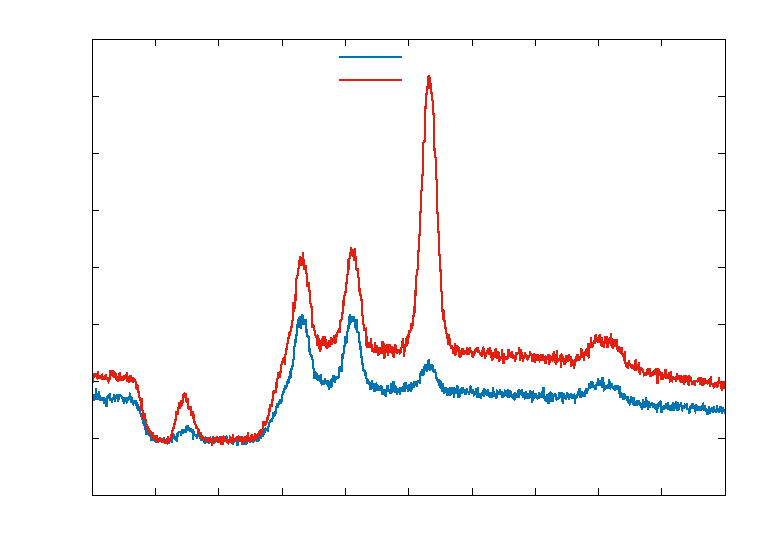
\includegraphics[width={360.00bp},height={252.00bp}]{Anhang/ccl4_as}}%
    \gplfronttext
  \end{picture}%
\endgroup
}}
    \caption{Gemessene Plots für Tetrachlormethan für $0^\circ$ und $90^\circ$-Polarisation im (Anti-)Stokes-Bereich}
\end{figure}\newpage
\section{Chlorophorm}
\begin{figure}[h]
    \centering\subfigure[Stokes Linien]{\scalebox{0.94}{% GNUPLOT: LaTeX picture with Postscript
\begingroup
  % Encoding inside the plot.  In the header of your document, this encoding
  % should to defined, e.g., by using
  % \usepackage[cp1252,<other encodings>]{inputenc}
  \inputencoding{cp1252}%
  \makeatletter
  \providecommand\color[2][]{%
    \GenericError{(gnuplot) \space\space\space\@spaces}{%
      Package color not loaded in conjunction with
      terminal option `colourtext'%
    }{See the gnuplot documentation for explanation.%
    }{Either use 'blacktext' in gnuplot or load the package
      color.sty in LaTeX.}%
    \renewcommand\color[2][]{}%
  }%
  \providecommand\includegraphics[2][]{%
    \GenericError{(gnuplot) \space\space\space\@spaces}{%
      Package graphicx or graphics not loaded%
    }{See the gnuplot documentation for explanation.%
    }{The gnuplot epslatex terminal needs graphicx.sty or graphics.sty.}%
    \renewcommand\includegraphics[2][]{}%
  }%
  \providecommand\rotatebox[2]{#2}%
  \@ifundefined{ifGPcolor}{%
    \newif\ifGPcolor
    \GPcolorfalse
  }{}%
  \@ifundefined{ifGPblacktext}{%
    \newif\ifGPblacktext
    \GPblacktexttrue
  }{}%
  % define a \g@addto@macro without @ in the name:
  \let\gplgaddtomacro\g@addto@macro
  % define empty templates for all commands taking text:
  \gdef\gplbacktext{}%
  \gdef\gplfronttext{}%
  \makeatother
  \ifGPblacktext
    % no textcolor at all
    \def\colorrgb#1{}%
    \def\colorgray#1{}%
  \else
    % gray or color?
    \ifGPcolor
      \def\colorrgb#1{\color[rgb]{#1}}%
      \def\colorgray#1{\color[gray]{#1}}%
      \expandafter\def\csname LTw\endcsname{\color{white}}%
      \expandafter\def\csname LTb\endcsname{\color{black}}%
      \expandafter\def\csname LTa\endcsname{\color{black}}%
      \expandafter\def\csname LT0\endcsname{\color[rgb]{1,0,0}}%
      \expandafter\def\csname LT1\endcsname{\color[rgb]{0,1,0}}%
      \expandafter\def\csname LT2\endcsname{\color[rgb]{0,0,1}}%
      \expandafter\def\csname LT3\endcsname{\color[rgb]{1,0,1}}%
      \expandafter\def\csname LT4\endcsname{\color[rgb]{0,1,1}}%
      \expandafter\def\csname LT5\endcsname{\color[rgb]{1,1,0}}%
      \expandafter\def\csname LT6\endcsname{\color[rgb]{0,0,0}}%
      \expandafter\def\csname LT7\endcsname{\color[rgb]{1,0.3,0}}%
      \expandafter\def\csname LT8\endcsname{\color[rgb]{0.5,0.5,0.5}}%
    \else
      % gray
      \def\colorrgb#1{\color{black}}%
      \def\colorgray#1{\color[gray]{#1}}%
      \expandafter\def\csname LTw\endcsname{\color{white}}%
      \expandafter\def\csname LTb\endcsname{\color{black}}%
      \expandafter\def\csname LTa\endcsname{\color{black}}%
      \expandafter\def\csname LT0\endcsname{\color{black}}%
      \expandafter\def\csname LT1\endcsname{\color{black}}%
      \expandafter\def\csname LT2\endcsname{\color{black}}%
      \expandafter\def\csname LT3\endcsname{\color{black}}%
      \expandafter\def\csname LT4\endcsname{\color{black}}%
      \expandafter\def\csname LT5\endcsname{\color{black}}%
      \expandafter\def\csname LT6\endcsname{\color{black}}%
      \expandafter\def\csname LT7\endcsname{\color{black}}%
      \expandafter\def\csname LT8\endcsname{\color{black}}%
    \fi
  \fi
    \setlength{\unitlength}{0.0500bp}%
    \ifx\gptboxheight\undefined%
      \newlength{\gptboxheight}%
      \newlength{\gptboxwidth}%
      \newsavebox{\gptboxtext}%
    \fi%
    \setlength{\fboxrule}{0.5pt}%
    \setlength{\fboxsep}{1pt}%
\begin{picture}(7200.00,5040.00)%
    \gplgaddtomacro\gplbacktext{%
      \csname LTb\endcsname%%
      \put(726,440){\makebox(0,0)[r]{\strut{}$0.08$}}%
      \put(726,1170){\makebox(0,0)[r]{\strut{}$0.1$}}%
      \put(726,1900){\makebox(0,0)[r]{\strut{}$0.12$}}%
      \put(726,2629){\makebox(0,0)[r]{\strut{}$0.14$}}%
      \put(726,3359){\makebox(0,0)[r]{\strut{}$0.16$}}%
      \put(726,4089){\makebox(0,0)[r]{\strut{}$0.18$}}%
      \put(726,4819){\makebox(0,0)[r]{\strut{}$0.2$}}%
      \put(858,220){\makebox(0,0){\strut{}$560$}}%
      \put(1601,220){\makebox(0,0){\strut{}$570$}}%
      \put(2344,220){\makebox(0,0){\strut{}$580$}}%
      \put(3087,220){\makebox(0,0){\strut{}$590$}}%
      \put(3831,220){\makebox(0,0){\strut{}$600$}}%
      \put(4574,220){\makebox(0,0){\strut{}$610$}}%
      \put(5317,220){\makebox(0,0){\strut{}$620$}}%
      \put(6060,220){\makebox(0,0){\strut{}$630$}}%
      \put(6803,220){\makebox(0,0){\strut{}$640$}}%
    }%
    \gplgaddtomacro\gplfronttext{%
      \csname LTb\endcsname%%
      \put(3102,4646){\makebox(0,0)[r]{\strut{}$0^\circ$ Polarisation}}%
      \csname LTb\endcsname%%
      \put(3102,4426){\makebox(0,0)[r]{\strut{}$90^\circ$ Polarisation}}%
    }%
    \gplbacktext
    \put(0,0){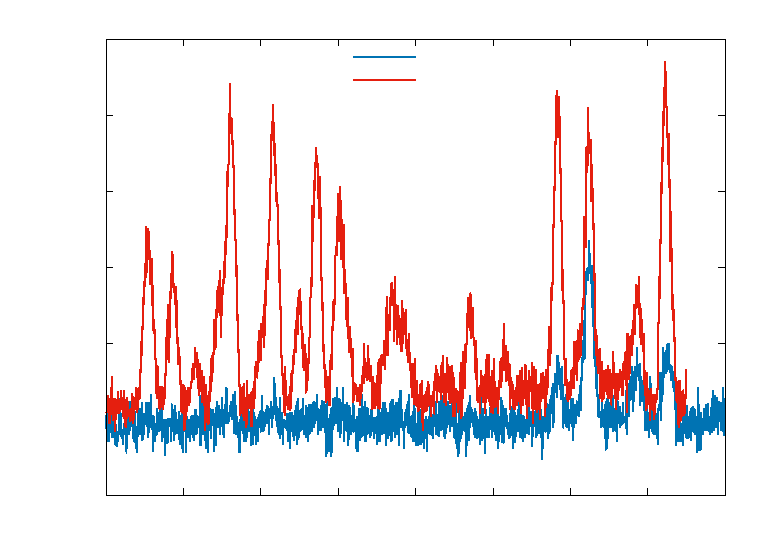
\includegraphics[width={360.00bp},height={252.00bp}]{Anhang/chcl3_s}}%
    \gplfronttext
  \end{picture}%
\endgroup
}}\\
    \subfigure[Anti-Stokes Linien]{\scalebox{0.94}{% GNUPLOT: LaTeX picture with Postscript
\begingroup
  % Encoding inside the plot.  In the header of your document, this encoding
  % should to defined, e.g., by using
  % \usepackage[cp1252,<other encodings>]{inputenc}
  \inputencoding{cp1252}%
  \makeatletter
  \providecommand\color[2][]{%
    \GenericError{(gnuplot) \space\space\space\@spaces}{%
      Package color not loaded in conjunction with
      terminal option `colourtext'%
    }{See the gnuplot documentation for explanation.%
    }{Either use 'blacktext' in gnuplot or load the package
      color.sty in LaTeX.}%
    \renewcommand\color[2][]{}%
  }%
  \providecommand\includegraphics[2][]{%
    \GenericError{(gnuplot) \space\space\space\@spaces}{%
      Package graphicx or graphics not loaded%
    }{See the gnuplot documentation for explanation.%
    }{The gnuplot epslatex terminal needs graphicx.sty or graphics.sty.}%
    \renewcommand\includegraphics[2][]{}%
  }%
  \providecommand\rotatebox[2]{#2}%
  \@ifundefined{ifGPcolor}{%
    \newif\ifGPcolor
    \GPcolorfalse
  }{}%
  \@ifundefined{ifGPblacktext}{%
    \newif\ifGPblacktext
    \GPblacktexttrue
  }{}%
  % define a \g@addto@macro without @ in the name:
  \let\gplgaddtomacro\g@addto@macro
  % define empty templates for all commands taking text:
  \gdef\gplbacktext{}%
  \gdef\gplfronttext{}%
  \makeatother
  \ifGPblacktext
    % no textcolor at all
    \def\colorrgb#1{}%
    \def\colorgray#1{}%
  \else
    % gray or color?
    \ifGPcolor
      \def\colorrgb#1{\color[rgb]{#1}}%
      \def\colorgray#1{\color[gray]{#1}}%
      \expandafter\def\csname LTw\endcsname{\color{white}}%
      \expandafter\def\csname LTb\endcsname{\color{black}}%
      \expandafter\def\csname LTa\endcsname{\color{black}}%
      \expandafter\def\csname LT0\endcsname{\color[rgb]{1,0,0}}%
      \expandafter\def\csname LT1\endcsname{\color[rgb]{0,1,0}}%
      \expandafter\def\csname LT2\endcsname{\color[rgb]{0,0,1}}%
      \expandafter\def\csname LT3\endcsname{\color[rgb]{1,0,1}}%
      \expandafter\def\csname LT4\endcsname{\color[rgb]{0,1,1}}%
      \expandafter\def\csname LT5\endcsname{\color[rgb]{1,1,0}}%
      \expandafter\def\csname LT6\endcsname{\color[rgb]{0,0,0}}%
      \expandafter\def\csname LT7\endcsname{\color[rgb]{1,0.3,0}}%
      \expandafter\def\csname LT8\endcsname{\color[rgb]{0.5,0.5,0.5}}%
    \else
      % gray
      \def\colorrgb#1{\color{black}}%
      \def\colorgray#1{\color[gray]{#1}}%
      \expandafter\def\csname LTw\endcsname{\color{white}}%
      \expandafter\def\csname LTb\endcsname{\color{black}}%
      \expandafter\def\csname LTa\endcsname{\color{black}}%
      \expandafter\def\csname LT0\endcsname{\color{black}}%
      \expandafter\def\csname LT1\endcsname{\color{black}}%
      \expandafter\def\csname LT2\endcsname{\color{black}}%
      \expandafter\def\csname LT3\endcsname{\color{black}}%
      \expandafter\def\csname LT4\endcsname{\color{black}}%
      \expandafter\def\csname LT5\endcsname{\color{black}}%
      \expandafter\def\csname LT6\endcsname{\color{black}}%
      \expandafter\def\csname LT7\endcsname{\color{black}}%
      \expandafter\def\csname LT8\endcsname{\color{black}}%
    \fi
  \fi
    \setlength{\unitlength}{0.0500bp}%
    \ifx\gptboxheight\undefined%
      \newlength{\gptboxheight}%
      \newlength{\gptboxwidth}%
      \newsavebox{\gptboxtext}%
    \fi%
    \setlength{\fboxrule}{0.5pt}%
    \setlength{\fboxsep}{1pt}%
\begin{picture}(7200.00,5040.00)%
    \gplgaddtomacro\gplbacktext{%
      \csname LTb\endcsname%%
      \put(726,440){\makebox(0,0)[r]{\strut{}$0.05$}}%
      \put(726,1066){\makebox(0,0)[r]{\strut{}$0.1$}}%
      \put(726,1691){\makebox(0,0)[r]{\strut{}$0.15$}}%
      \put(726,2317){\makebox(0,0)[r]{\strut{}$0.2$}}%
      \put(726,2942){\makebox(0,0)[r]{\strut{}$0.25$}}%
      \put(726,3568){\makebox(0,0)[r]{\strut{}$0.3$}}%
      \put(726,4193){\makebox(0,0)[r]{\strut{}$0.35$}}%
      \put(726,4819){\makebox(0,0)[r]{\strut{}$0.4$}}%
      \put(858,220){\makebox(0,0){\strut{}$620$}}%
      \put(1707,220){\makebox(0,0){\strut{}$630$}}%
      \put(2557,220){\makebox(0,0){\strut{}$640$}}%
      \put(3406,220){\makebox(0,0){\strut{}$650$}}%
      \put(4255,220){\makebox(0,0){\strut{}$660$}}%
      \put(5104,220){\makebox(0,0){\strut{}$670$}}%
      \put(5954,220){\makebox(0,0){\strut{}$680$}}%
      \put(6803,220){\makebox(0,0){\strut{}$690$}}%
    }%
    \gplgaddtomacro\gplfronttext{%
      \csname LTb\endcsname%%
      \put(3102,4646){\makebox(0,0)[r]{\strut{}$0^\circ$ Polarisation}}%
      \csname LTb\endcsname%%
      \put(3102,4426){\makebox(0,0)[r]{\strut{}$90^\circ$ Polarisation}}%
    }%
    \gplbacktext
    \put(0,0){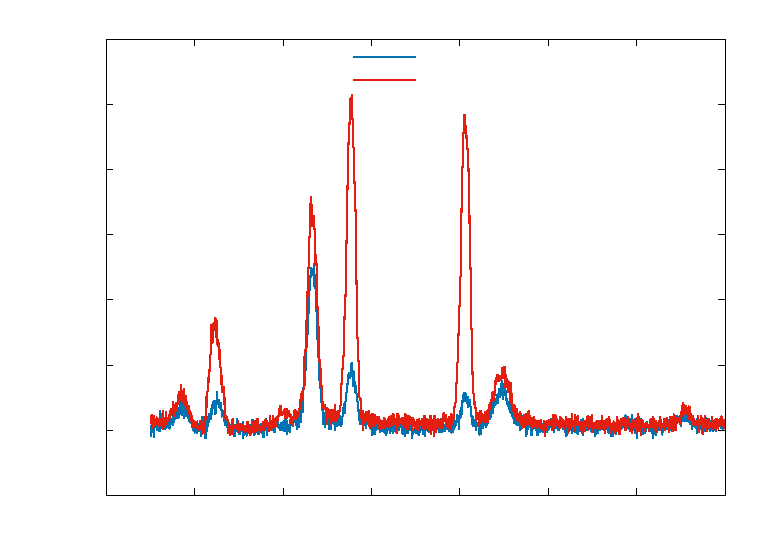
\includegraphics[width={360.00bp},height={252.00bp}]{Anhang/chcl3_as}}%
    \gplfronttext
  \end{picture}%
\endgroup
}}
    \caption{Gemessene Plots für Chlorophorm für $0^\circ$ und $90^\circ$-Polarisation im (Anti-)Stokes-Bereich}
\end{figure}\newpage
\section{Deuterium Chlorophorm}
\begin{figure}[h]
    \centering\subfigure[Stokes Linien]{\scalebox{0.94}{% GNUPLOT: LaTeX picture with Postscript
\begingroup
  % Encoding inside the plot.  In the header of your document, this encoding
  % should to defined, e.g., by using
  % \usepackage[cp1252,<other encodings>]{inputenc}
  \inputencoding{cp1252}%
  \makeatletter
  \providecommand\color[2][]{%
    \GenericError{(gnuplot) \space\space\space\@spaces}{%
      Package color not loaded in conjunction with
      terminal option `colourtext'%
    }{See the gnuplot documentation for explanation.%
    }{Either use 'blacktext' in gnuplot or load the package
      color.sty in LaTeX.}%
    \renewcommand\color[2][]{}%
  }%
  \providecommand\includegraphics[2][]{%
    \GenericError{(gnuplot) \space\space\space\@spaces}{%
      Package graphicx or graphics not loaded%
    }{See the gnuplot documentation for explanation.%
    }{The gnuplot epslatex terminal needs graphicx.sty or graphics.sty.}%
    \renewcommand\includegraphics[2][]{}%
  }%
  \providecommand\rotatebox[2]{#2}%
  \@ifundefined{ifGPcolor}{%
    \newif\ifGPcolor
    \GPcolorfalse
  }{}%
  \@ifundefined{ifGPblacktext}{%
    \newif\ifGPblacktext
    \GPblacktexttrue
  }{}%
  % define a \g@addto@macro without @ in the name:
  \let\gplgaddtomacro\g@addto@macro
  % define empty templates for all commands taking text:
  \gdef\gplbacktext{}%
  \gdef\gplfronttext{}%
  \makeatother
  \ifGPblacktext
    % no textcolor at all
    \def\colorrgb#1{}%
    \def\colorgray#1{}%
  \else
    % gray or color?
    \ifGPcolor
      \def\colorrgb#1{\color[rgb]{#1}}%
      \def\colorgray#1{\color[gray]{#1}}%
      \expandafter\def\csname LTw\endcsname{\color{white}}%
      \expandafter\def\csname LTb\endcsname{\color{black}}%
      \expandafter\def\csname LTa\endcsname{\color{black}}%
      \expandafter\def\csname LT0\endcsname{\color[rgb]{1,0,0}}%
      \expandafter\def\csname LT1\endcsname{\color[rgb]{0,1,0}}%
      \expandafter\def\csname LT2\endcsname{\color[rgb]{0,0,1}}%
      \expandafter\def\csname LT3\endcsname{\color[rgb]{1,0,1}}%
      \expandafter\def\csname LT4\endcsname{\color[rgb]{0,1,1}}%
      \expandafter\def\csname LT5\endcsname{\color[rgb]{1,1,0}}%
      \expandafter\def\csname LT6\endcsname{\color[rgb]{0,0,0}}%
      \expandafter\def\csname LT7\endcsname{\color[rgb]{1,0.3,0}}%
      \expandafter\def\csname LT8\endcsname{\color[rgb]{0.5,0.5,0.5}}%
    \else
      % gray
      \def\colorrgb#1{\color{black}}%
      \def\colorgray#1{\color[gray]{#1}}%
      \expandafter\def\csname LTw\endcsname{\color{white}}%
      \expandafter\def\csname LTb\endcsname{\color{black}}%
      \expandafter\def\csname LTa\endcsname{\color{black}}%
      \expandafter\def\csname LT0\endcsname{\color{black}}%
      \expandafter\def\csname LT1\endcsname{\color{black}}%
      \expandafter\def\csname LT2\endcsname{\color{black}}%
      \expandafter\def\csname LT3\endcsname{\color{black}}%
      \expandafter\def\csname LT4\endcsname{\color{black}}%
      \expandafter\def\csname LT5\endcsname{\color{black}}%
      \expandafter\def\csname LT6\endcsname{\color{black}}%
      \expandafter\def\csname LT7\endcsname{\color{black}}%
      \expandafter\def\csname LT8\endcsname{\color{black}}%
    \fi
  \fi
    \setlength{\unitlength}{0.0500bp}%
    \ifx\gptboxheight\undefined%
      \newlength{\gptboxheight}%
      \newlength{\gptboxwidth}%
      \newsavebox{\gptboxtext}%
    \fi%
    \setlength{\fboxrule}{0.5pt}%
    \setlength{\fboxsep}{1pt}%
\begin{picture}(7200.00,5040.00)%
    \gplgaddtomacro\gplbacktext{%
      \csname LTb\endcsname%%
      \put(726,440){\makebox(0,0)[r]{\strut{}$0.06$}}%
      \put(726,1066){\makebox(0,0)[r]{\strut{}$0.08$}}%
      \put(726,1691){\makebox(0,0)[r]{\strut{}$0.1$}}%
      \put(726,2317){\makebox(0,0)[r]{\strut{}$0.12$}}%
      \put(726,2942){\makebox(0,0)[r]{\strut{}$0.14$}}%
      \put(726,3568){\makebox(0,0)[r]{\strut{}$0.16$}}%
      \put(726,4193){\makebox(0,0)[r]{\strut{}$0.18$}}%
      \put(726,4819){\makebox(0,0)[r]{\strut{}$0.2$}}%
      \put(858,220){\makebox(0,0){\strut{}$570$}}%
      \put(1707,220){\makebox(0,0){\strut{}$580$}}%
      \put(2557,220){\makebox(0,0){\strut{}$590$}}%
      \put(3406,220){\makebox(0,0){\strut{}$600$}}%
      \put(4255,220){\makebox(0,0){\strut{}$610$}}%
      \put(5104,220){\makebox(0,0){\strut{}$620$}}%
      \put(5954,220){\makebox(0,0){\strut{}$630$}}%
      \put(6803,220){\makebox(0,0){\strut{}$640$}}%
    }%
    \gplgaddtomacro\gplfronttext{%
      \csname LTb\endcsname%%
      \put(3102,4646){\makebox(0,0)[r]{\strut{}$0^\circ$ Polarisation}}%
      \csname LTb\endcsname%%
      \put(3102,4426){\makebox(0,0)[r]{\strut{}$90^\circ$ Polarisation}}%
    }%
    \gplbacktext
    \put(0,0){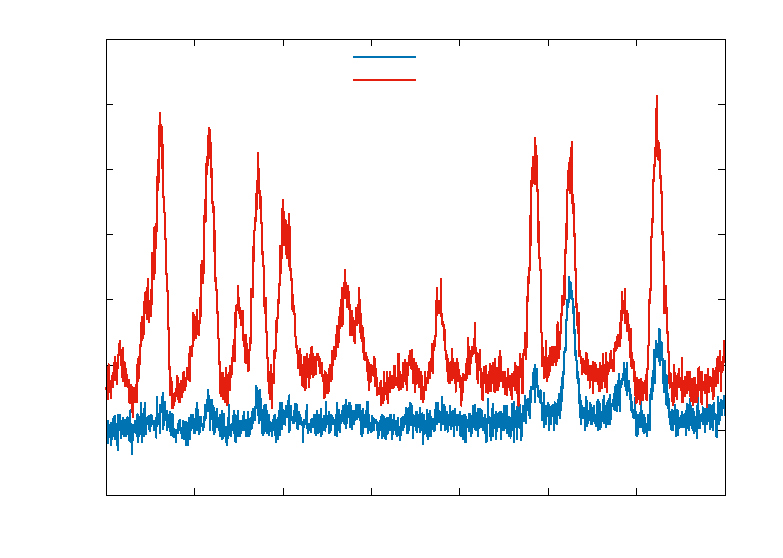
\includegraphics[width={360.00bp},height={252.00bp}]{Anhang/cdcl3_s}}%
    \gplfronttext
  \end{picture}%
\endgroup
}}\\
    \subfigure[Anti-Stokes Linien]{\scalebox{0.94}{% GNUPLOT: LaTeX picture with Postscript
\begingroup
  % Encoding inside the plot.  In the header of your document, this encoding
  % should to defined, e.g., by using
  % \usepackage[cp1252,<other encodings>]{inputenc}
  \inputencoding{cp1252}%
  \makeatletter
  \providecommand\color[2][]{%
    \GenericError{(gnuplot) \space\space\space\@spaces}{%
      Package color not loaded in conjunction with
      terminal option `colourtext'%
    }{See the gnuplot documentation for explanation.%
    }{Either use 'blacktext' in gnuplot or load the package
      color.sty in LaTeX.}%
    \renewcommand\color[2][]{}%
  }%
  \providecommand\includegraphics[2][]{%
    \GenericError{(gnuplot) \space\space\space\@spaces}{%
      Package graphicx or graphics not loaded%
    }{See the gnuplot documentation for explanation.%
    }{The gnuplot epslatex terminal needs graphicx.sty or graphics.sty.}%
    \renewcommand\includegraphics[2][]{}%
  }%
  \providecommand\rotatebox[2]{#2}%
  \@ifundefined{ifGPcolor}{%
    \newif\ifGPcolor
    \GPcolorfalse
  }{}%
  \@ifundefined{ifGPblacktext}{%
    \newif\ifGPblacktext
    \GPblacktexttrue
  }{}%
  % define a \g@addto@macro without @ in the name:
  \let\gplgaddtomacro\g@addto@macro
  % define empty templates for all commands taking text:
  \gdef\gplbacktext{}%
  \gdef\gplfronttext{}%
  \makeatother
  \ifGPblacktext
    % no textcolor at all
    \def\colorrgb#1{}%
    \def\colorgray#1{}%
  \else
    % gray or color?
    \ifGPcolor
      \def\colorrgb#1{\color[rgb]{#1}}%
      \def\colorgray#1{\color[gray]{#1}}%
      \expandafter\def\csname LTw\endcsname{\color{white}}%
      \expandafter\def\csname LTb\endcsname{\color{black}}%
      \expandafter\def\csname LTa\endcsname{\color{black}}%
      \expandafter\def\csname LT0\endcsname{\color[rgb]{1,0,0}}%
      \expandafter\def\csname LT1\endcsname{\color[rgb]{0,1,0}}%
      \expandafter\def\csname LT2\endcsname{\color[rgb]{0,0,1}}%
      \expandafter\def\csname LT3\endcsname{\color[rgb]{1,0,1}}%
      \expandafter\def\csname LT4\endcsname{\color[rgb]{0,1,1}}%
      \expandafter\def\csname LT5\endcsname{\color[rgb]{1,1,0}}%
      \expandafter\def\csname LT6\endcsname{\color[rgb]{0,0,0}}%
      \expandafter\def\csname LT7\endcsname{\color[rgb]{1,0.3,0}}%
      \expandafter\def\csname LT8\endcsname{\color[rgb]{0.5,0.5,0.5}}%
    \else
      % gray
      \def\colorrgb#1{\color{black}}%
      \def\colorgray#1{\color[gray]{#1}}%
      \expandafter\def\csname LTw\endcsname{\color{white}}%
      \expandafter\def\csname LTb\endcsname{\color{black}}%
      \expandafter\def\csname LTa\endcsname{\color{black}}%
      \expandafter\def\csname LT0\endcsname{\color{black}}%
      \expandafter\def\csname LT1\endcsname{\color{black}}%
      \expandafter\def\csname LT2\endcsname{\color{black}}%
      \expandafter\def\csname LT3\endcsname{\color{black}}%
      \expandafter\def\csname LT4\endcsname{\color{black}}%
      \expandafter\def\csname LT5\endcsname{\color{black}}%
      \expandafter\def\csname LT6\endcsname{\color{black}}%
      \expandafter\def\csname LT7\endcsname{\color{black}}%
      \expandafter\def\csname LT8\endcsname{\color{black}}%
    \fi
  \fi
    \setlength{\unitlength}{0.0500bp}%
    \ifx\gptboxheight\undefined%
      \newlength{\gptboxheight}%
      \newlength{\gptboxwidth}%
      \newsavebox{\gptboxtext}%
    \fi%
    \setlength{\fboxrule}{0.5pt}%
    \setlength{\fboxsep}{1pt}%
\begin{picture}(7200.00,5040.00)%
    \gplgaddtomacro\gplbacktext{%
      \csname LTb\endcsname%%
      \put(726,440){\makebox(0,0)[r]{\strut{}$0.05$}}%
      \put(726,1066){\makebox(0,0)[r]{\strut{}$0.1$}}%
      \put(726,1691){\makebox(0,0)[r]{\strut{}$0.15$}}%
      \put(726,2317){\makebox(0,0)[r]{\strut{}$0.2$}}%
      \put(726,2942){\makebox(0,0)[r]{\strut{}$0.25$}}%
      \put(726,3568){\makebox(0,0)[r]{\strut{}$0.3$}}%
      \put(726,4193){\makebox(0,0)[r]{\strut{}$0.35$}}%
      \put(726,4819){\makebox(0,0)[r]{\strut{}$0.4$}}%
      \put(858,220){\makebox(0,0){\strut{}$620$}}%
      \put(1601,220){\makebox(0,0){\strut{}$630$}}%
      \put(2344,220){\makebox(0,0){\strut{}$640$}}%
      \put(3087,220){\makebox(0,0){\strut{}$650$}}%
      \put(3831,220){\makebox(0,0){\strut{}$660$}}%
      \put(4574,220){\makebox(0,0){\strut{}$670$}}%
      \put(5317,220){\makebox(0,0){\strut{}$680$}}%
      \put(6060,220){\makebox(0,0){\strut{}$690$}}%
      \put(6803,220){\makebox(0,0){\strut{}$700$}}%
    }%
    \gplgaddtomacro\gplfronttext{%
      \csname LTb\endcsname%%
      \put(3102,4646){\makebox(0,0)[r]{\strut{}$0^\circ$ Polarisation}}%
      \csname LTb\endcsname%%
      \put(3102,4426){\makebox(0,0)[r]{\strut{}$90^\circ$ Polarisation}}%
    }%
    \gplbacktext
    \put(0,0){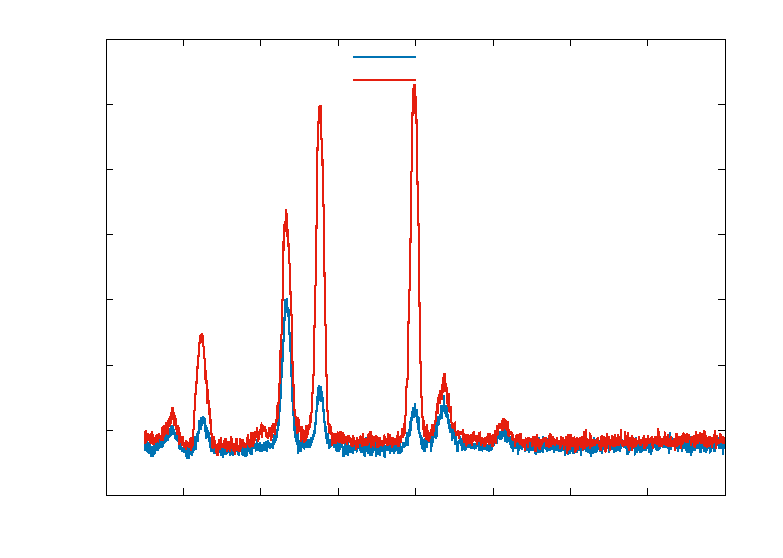
\includegraphics[width={360.00bp},height={252.00bp}]{Anhang/cdcl3_as}}%
    \gplfronttext
  \end{picture}%
\endgroup
}}
    \caption{Gemessene Plots für Deuterium Chlorophorm für $0^\circ$ und $90^\circ$-Polarisation im (Anti-)Stokes-Bereich}
\end{figure}\newpage
\section{Bromophorm}
\begin{figure}[h]
    \centering\subfigure[Stokes Linien]{\scalebox{0.94}{% GNUPLOT: LaTeX picture with Postscript
\begingroup
  % Encoding inside the plot.  In the header of your document, this encoding
  % should to defined, e.g., by using
  % \usepackage[cp1252,<other encodings>]{inputenc}
  \inputencoding{cp1252}%
  \makeatletter
  \providecommand\color[2][]{%
    \GenericError{(gnuplot) \space\space\space\@spaces}{%
      Package color not loaded in conjunction with
      terminal option `colourtext'%
    }{See the gnuplot documentation for explanation.%
    }{Either use 'blacktext' in gnuplot or load the package
      color.sty in LaTeX.}%
    \renewcommand\color[2][]{}%
  }%
  \providecommand\includegraphics[2][]{%
    \GenericError{(gnuplot) \space\space\space\@spaces}{%
      Package graphicx or graphics not loaded%
    }{See the gnuplot documentation for explanation.%
    }{The gnuplot epslatex terminal needs graphicx.sty or graphics.sty.}%
    \renewcommand\includegraphics[2][]{}%
  }%
  \providecommand\rotatebox[2]{#2}%
  \@ifundefined{ifGPcolor}{%
    \newif\ifGPcolor
    \GPcolorfalse
  }{}%
  \@ifundefined{ifGPblacktext}{%
    \newif\ifGPblacktext
    \GPblacktexttrue
  }{}%
  % define a \g@addto@macro without @ in the name:
  \let\gplgaddtomacro\g@addto@macro
  % define empty templates for all commands taking text:
  \gdef\gplbacktext{}%
  \gdef\gplfronttext{}%
  \makeatother
  \ifGPblacktext
    % no textcolor at all
    \def\colorrgb#1{}%
    \def\colorgray#1{}%
  \else
    % gray or color?
    \ifGPcolor
      \def\colorrgb#1{\color[rgb]{#1}}%
      \def\colorgray#1{\color[gray]{#1}}%
      \expandafter\def\csname LTw\endcsname{\color{white}}%
      \expandafter\def\csname LTb\endcsname{\color{black}}%
      \expandafter\def\csname LTa\endcsname{\color{black}}%
      \expandafter\def\csname LT0\endcsname{\color[rgb]{1,0,0}}%
      \expandafter\def\csname LT1\endcsname{\color[rgb]{0,1,0}}%
      \expandafter\def\csname LT2\endcsname{\color[rgb]{0,0,1}}%
      \expandafter\def\csname LT3\endcsname{\color[rgb]{1,0,1}}%
      \expandafter\def\csname LT4\endcsname{\color[rgb]{0,1,1}}%
      \expandafter\def\csname LT5\endcsname{\color[rgb]{1,1,0}}%
      \expandafter\def\csname LT6\endcsname{\color[rgb]{0,0,0}}%
      \expandafter\def\csname LT7\endcsname{\color[rgb]{1,0.3,0}}%
      \expandafter\def\csname LT8\endcsname{\color[rgb]{0.5,0.5,0.5}}%
    \else
      % gray
      \def\colorrgb#1{\color{black}}%
      \def\colorgray#1{\color[gray]{#1}}%
      \expandafter\def\csname LTw\endcsname{\color{white}}%
      \expandafter\def\csname LTb\endcsname{\color{black}}%
      \expandafter\def\csname LTa\endcsname{\color{black}}%
      \expandafter\def\csname LT0\endcsname{\color{black}}%
      \expandafter\def\csname LT1\endcsname{\color{black}}%
      \expandafter\def\csname LT2\endcsname{\color{black}}%
      \expandafter\def\csname LT3\endcsname{\color{black}}%
      \expandafter\def\csname LT4\endcsname{\color{black}}%
      \expandafter\def\csname LT5\endcsname{\color{black}}%
      \expandafter\def\csname LT6\endcsname{\color{black}}%
      \expandafter\def\csname LT7\endcsname{\color{black}}%
      \expandafter\def\csname LT8\endcsname{\color{black}}%
    \fi
  \fi
    \setlength{\unitlength}{0.0500bp}%
    \ifx\gptboxheight\undefined%
      \newlength{\gptboxheight}%
      \newlength{\gptboxwidth}%
      \newsavebox{\gptboxtext}%
    \fi%
    \setlength{\fboxrule}{0.5pt}%
    \setlength{\fboxsep}{1pt}%
\begin{picture}(7200.00,5040.00)%
    \gplgaddtomacro\gplbacktext{%
      \csname LTb\endcsname%%
      \put(726,440){\makebox(0,0)[r]{\strut{}$0.05$}}%
      \put(726,927){\makebox(0,0)[r]{\strut{}$0.1$}}%
      \put(726,1413){\makebox(0,0)[r]{\strut{}$0.15$}}%
      \put(726,1900){\makebox(0,0)[r]{\strut{}$0.2$}}%
      \put(726,2386){\makebox(0,0)[r]{\strut{}$0.25$}}%
      \put(726,2873){\makebox(0,0)[r]{\strut{}$0.3$}}%
      \put(726,3359){\makebox(0,0)[r]{\strut{}$0.35$}}%
      \put(726,3846){\makebox(0,0)[r]{\strut{}$0.4$}}%
      \put(726,4332){\makebox(0,0)[r]{\strut{}$0.45$}}%
      \put(726,4819){\makebox(0,0)[r]{\strut{}$0.5$}}%
      \put(858,220){\makebox(0,0){\strut{}$560$}}%
      \put(1601,220){\makebox(0,0){\strut{}$570$}}%
      \put(2344,220){\makebox(0,0){\strut{}$580$}}%
      \put(3087,220){\makebox(0,0){\strut{}$590$}}%
      \put(3831,220){\makebox(0,0){\strut{}$600$}}%
      \put(4574,220){\makebox(0,0){\strut{}$610$}}%
      \put(5317,220){\makebox(0,0){\strut{}$620$}}%
      \put(6060,220){\makebox(0,0){\strut{}$630$}}%
      \put(6803,220){\makebox(0,0){\strut{}$640$}}%
    }%
    \gplgaddtomacro\gplfronttext{%
      \csname LTb\endcsname%%
      \put(3102,4646){\makebox(0,0)[r]{\strut{}$0^\circ$ Polarisation}}%
      \csname LTb\endcsname%%
      \put(3102,4426){\makebox(0,0)[r]{\strut{}$90^\circ$ Polarisation}}%
    }%
    \gplbacktext
    \put(0,0){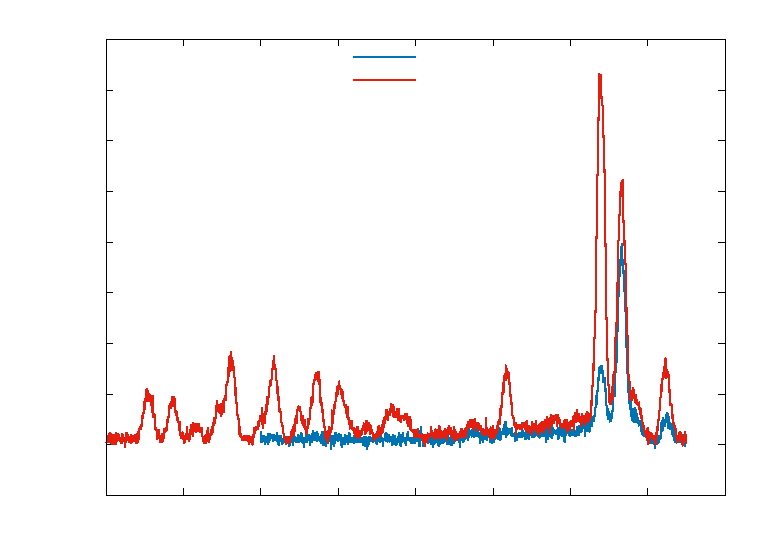
\includegraphics[width={360.00bp},height={252.00bp}]{Anhang/chbr3_s}}%
    \gplfronttext
  \end{picture}%
\endgroup
}}\\
    \subfigure[Anti-Stokes Linien]{\scalebox{0.94}{% GNUPLOT: LaTeX picture with Postscript
\begingroup
  % Encoding inside the plot.  In the header of your document, this encoding
  % should to defined, e.g., by using
  % \usepackage[cp1252,<other encodings>]{inputenc}
  \inputencoding{cp1252}%
  \makeatletter
  \providecommand\color[2][]{%
    \GenericError{(gnuplot) \space\space\space\@spaces}{%
      Package color not loaded in conjunction with
      terminal option `colourtext'%
    }{See the gnuplot documentation for explanation.%
    }{Either use 'blacktext' in gnuplot or load the package
      color.sty in LaTeX.}%
    \renewcommand\color[2][]{}%
  }%
  \providecommand\includegraphics[2][]{%
    \GenericError{(gnuplot) \space\space\space\@spaces}{%
      Package graphicx or graphics not loaded%
    }{See the gnuplot documentation for explanation.%
    }{The gnuplot epslatex terminal needs graphicx.sty or graphics.sty.}%
    \renewcommand\includegraphics[2][]{}%
  }%
  \providecommand\rotatebox[2]{#2}%
  \@ifundefined{ifGPcolor}{%
    \newif\ifGPcolor
    \GPcolorfalse
  }{}%
  \@ifundefined{ifGPblacktext}{%
    \newif\ifGPblacktext
    \GPblacktexttrue
  }{}%
  % define a \g@addto@macro without @ in the name:
  \let\gplgaddtomacro\g@addto@macro
  % define empty templates for all commands taking text:
  \gdef\gplbacktext{}%
  \gdef\gplfronttext{}%
  \makeatother
  \ifGPblacktext
    % no textcolor at all
    \def\colorrgb#1{}%
    \def\colorgray#1{}%
  \else
    % gray or color?
    \ifGPcolor
      \def\colorrgb#1{\color[rgb]{#1}}%
      \def\colorgray#1{\color[gray]{#1}}%
      \expandafter\def\csname LTw\endcsname{\color{white}}%
      \expandafter\def\csname LTb\endcsname{\color{black}}%
      \expandafter\def\csname LTa\endcsname{\color{black}}%
      \expandafter\def\csname LT0\endcsname{\color[rgb]{1,0,0}}%
      \expandafter\def\csname LT1\endcsname{\color[rgb]{0,1,0}}%
      \expandafter\def\csname LT2\endcsname{\color[rgb]{0,0,1}}%
      \expandafter\def\csname LT3\endcsname{\color[rgb]{1,0,1}}%
      \expandafter\def\csname LT4\endcsname{\color[rgb]{0,1,1}}%
      \expandafter\def\csname LT5\endcsname{\color[rgb]{1,1,0}}%
      \expandafter\def\csname LT6\endcsname{\color[rgb]{0,0,0}}%
      \expandafter\def\csname LT7\endcsname{\color[rgb]{1,0.3,0}}%
      \expandafter\def\csname LT8\endcsname{\color[rgb]{0.5,0.5,0.5}}%
    \else
      % gray
      \def\colorrgb#1{\color{black}}%
      \def\colorgray#1{\color[gray]{#1}}%
      \expandafter\def\csname LTw\endcsname{\color{white}}%
      \expandafter\def\csname LTb\endcsname{\color{black}}%
      \expandafter\def\csname LTa\endcsname{\color{black}}%
      \expandafter\def\csname LT0\endcsname{\color{black}}%
      \expandafter\def\csname LT1\endcsname{\color{black}}%
      \expandafter\def\csname LT2\endcsname{\color{black}}%
      \expandafter\def\csname LT3\endcsname{\color{black}}%
      \expandafter\def\csname LT4\endcsname{\color{black}}%
      \expandafter\def\csname LT5\endcsname{\color{black}}%
      \expandafter\def\csname LT6\endcsname{\color{black}}%
      \expandafter\def\csname LT7\endcsname{\color{black}}%
      \expandafter\def\csname LT8\endcsname{\color{black}}%
    \fi
  \fi
    \setlength{\unitlength}{0.0500bp}%
    \ifx\gptboxheight\undefined%
      \newlength{\gptboxheight}%
      \newlength{\gptboxwidth}%
      \newsavebox{\gptboxtext}%
    \fi%
    \setlength{\fboxrule}{0.5pt}%
    \setlength{\fboxsep}{1pt}%
\begin{picture}(7200.00,5040.00)%
    \gplgaddtomacro\gplbacktext{%
      \csname LTb\endcsname%%
      \put(594,440){\makebox(0,0)[r]{\strut{}$0$}}%
      \put(594,927){\makebox(0,0)[r]{\strut{}$0.1$}}%
      \put(594,1413){\makebox(0,0)[r]{\strut{}$0.2$}}%
      \put(594,1900){\makebox(0,0)[r]{\strut{}$0.3$}}%
      \put(594,2386){\makebox(0,0)[r]{\strut{}$0.4$}}%
      \put(594,2873){\makebox(0,0)[r]{\strut{}$0.5$}}%
      \put(594,3359){\makebox(0,0)[r]{\strut{}$0.6$}}%
      \put(594,3846){\makebox(0,0)[r]{\strut{}$0.7$}}%
      \put(594,4332){\makebox(0,0)[r]{\strut{}$0.8$}}%
      \put(594,4819){\makebox(0,0)[r]{\strut{}$0.9$}}%
      \put(726,220){\makebox(0,0){\strut{}$620$}}%
      \put(1594,220){\makebox(0,0){\strut{}$630$}}%
      \put(2462,220){\makebox(0,0){\strut{}$640$}}%
      \put(3330,220){\makebox(0,0){\strut{}$650$}}%
      \put(4199,220){\makebox(0,0){\strut{}$660$}}%
      \put(5067,220){\makebox(0,0){\strut{}$670$}}%
      \put(5935,220){\makebox(0,0){\strut{}$680$}}%
      \put(6803,220){\makebox(0,0){\strut{}$690$}}%
    }%
    \gplgaddtomacro\gplfronttext{%
      \csname LTb\endcsname%%
      \put(5816,4646){\makebox(0,0)[r]{\strut{}$0^\circ$ Polarisation}}%
      \csname LTb\endcsname%%
      \put(5816,4426){\makebox(0,0)[r]{\strut{}$90^\circ$ Polarisation}}%
    }%
    \gplbacktext
    \put(0,0){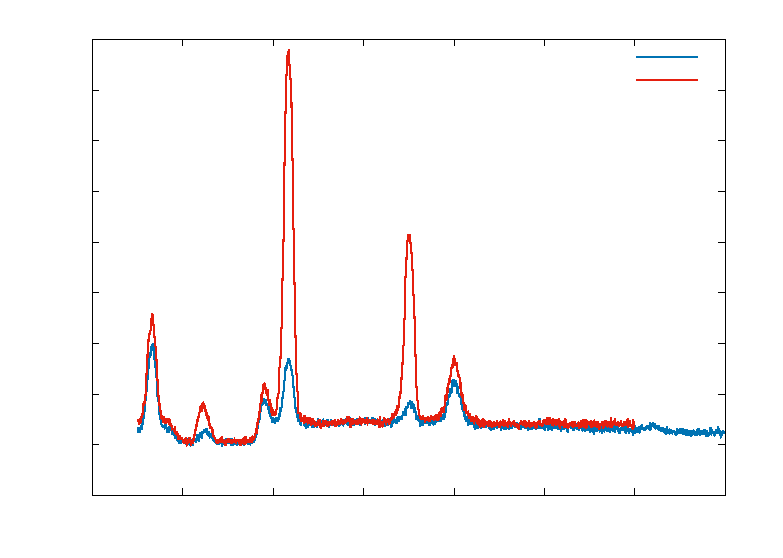
\includegraphics[width={360.00bp},height={252.00bp}]{Anhang/chbr3_as}}%
    \gplfronttext
  \end{picture}%
\endgroup
}}
    \caption{Gemessene Plots für Bromophorm für $0^\circ$ und $90^\circ$-Polarisation im (Anti-)Stokes-Bereich}
\end{figure}\newpage

%Literatur
\cleardoublepage
\bibliography{Literatur/Literatur}
\bibliographystyle{Literatur/LAuswertung}

%\newpage
%\listoffigures

\end{document}
%
% ------------------------------ Ende des Dokumentes -----------------------------------------
